% \documentclass{article}
% \usepackage{amsmath}
% \usepackage{amsthm}
% \usepackage{enumerate}
% \usepackage{bookmark}
% \usepackage{graphicx}
% \usepackage{multirow}
% \usepackage{adjustbox}
% \usepackage{wrapfig}
% \usepackage{subcaption}
% \usepackage{color}
% \usepackage[dvipsnames]{xcolor}

% \usepackage{amssymb,amsmath,amsthm,amsfonts}
% \usepackage{mathrsfs}
% \usepackage{dsfont}
% \usepackage{enumerate}

% \usepackage{amssymb,amsmath,amsthm,amsfonts}
\usepackage{mathrsfs}
\usepackage{dsfont}
\usepackage{enumerate}

%\newtheorem{mdef}{Definition}
%\newtheorem{theorem}{Theorem}
\newcommand{\eqsplit}[2]{
  \begin{equation}\label{#2}
    \begin{split}
      #1
    \end{split}
  \end{equation}}
\newcommand{\eqnsplit}[1]{
  \begin{eqnarray*}
    #1
  \end{eqnarray*}}
\newcommand{\tran}[1]{
  \tilde{#1}
}
\newcommand{\td}[2]{
  \frac{d #1}{d #2}
}
\newcommand{\pd}[2]{
  \frac{\partial #1}{\partial #2}
}
\newcommand{\ppd}[2]{
  \frac{\partial^2 #1}{\partial #2^2}
}
\newcommand{\pdd}[3]{
  \frac{\partial^2 #1}{\partial #2 \partial #3}
}
\newcommand{\otd}[1]{
  \frac{d}{d #1}
}
\newcommand{\opd}[1]{
  \frac{\partial}{\partial #1}
}
\newcommand{\oppd}[1]{
  \frac{\partial^2}{\partial #1^2}
}
\newcommand{\opdd}[2]{
  \frac{\partial^2}{\partial #1 \partial #2}
}
\newcommand{\ket}[1]{
  |#1\rangle
}
\newcommand{\bra}[1]{
  \langle#1|
}
\newcommand{\inn}[1]{
  \langle#1\rangle
}
\newcommand{\mean}[1]{
  \langle#1\rangle
}
\newcommand{\tr}{
  \text{tr}\,
}
\newcommand{\re}{
  \text{Re}\,
}
\newcommand\im{
  \text{Im}\,
}
\newcommand{\var}{
  \text{var}
}
\newcommand{\arcsinh}{
  \sinh^{-1}
}
\newcommand{\arccosh}{
  \cosh^{-1}
}
\newcommand{\erfc}{
  \text{erfc}
}
\newcommand{\E}{
  \mathbb{E}
}
\renewcommand{\P}{
  \mathbb{P}
}
\newcommand{\I}[1]{
  \mathbf{1}_{\{#1\}}
}
\newcommand{\1}[1]{
  \mathds{1}_{\{#1\}}
}
\newcommand{\diag}{
  \text{diag\,}
}
\newcommand{\M}{
  {\text{max}}
}
\newcommand{\m}{
  {\text{min}}
}
\newcommand{\ph}{
  {\text{arg}\,}
}
\newcommand\erf{
  \text{erf}
}
\renewcommand\vec[1]{
  \mathbf{#1}
}
\newcommand\mtx[1]{
  \mathbf{#1}
}
\newcommand\ed{
  \,{\buildrel d \over =}\,
}





\documentclass[11pt,a4]{amsart}
%\usepackage{amsmath}
%\usepackage{amsthm}
%\usepackage{enumerate}
% \usepackage[bookmarks=true]{hyperref}
%% \usepackage{bookmark}
\usepackage{graphicx}
%\usepackage{multirow}
%\usepackage{adjustbox}
%\usepackage{wrapfig}
%\usepackage{subcaption}
\usepackage{color}
\usepackage[dvipsnames]{xcolor}

\usepackage{amssymb,amsmath,amsthm,amsfonts}
%\usepackage{mathrsfs}
%\usepackage{dsfont}
%\usepackage{enumerate}

%\usepackage{amssymb,amsmath,amsthm,amsfonts}
\usepackage{mathrsfs}
\usepackage{dsfont}
\usepackage{enumerate}

%\newtheorem{mdef}{Definition}
%\newtheorem{theorem}{Theorem}
\newcommand{\eqsplit}[2]{
  \begin{equation}\label{#2}
    \begin{split}
      #1
    \end{split}
  \end{equation}}
\newcommand{\eqnsplit}[1]{
  \begin{eqnarray*}
    #1
  \end{eqnarray*}}
\newcommand{\tran}[1]{
  \tilde{#1}
}
\newcommand{\td}[2]{
  \frac{d #1}{d #2}
}
\newcommand{\pd}[2]{
  \frac{\partial #1}{\partial #2}
}
\newcommand{\ppd}[2]{
  \frac{\partial^2 #1}{\partial #2^2}
}
\newcommand{\pdd}[3]{
  \frac{\partial^2 #1}{\partial #2 \partial #3}
}
\newcommand{\otd}[1]{
  \frac{d}{d #1}
}
\newcommand{\opd}[1]{
  \frac{\partial}{\partial #1}
}
\newcommand{\oppd}[1]{
  \frac{\partial^2}{\partial #1^2}
}
\newcommand{\opdd}[2]{
  \frac{\partial^2}{\partial #1 \partial #2}
}
\newcommand{\ket}[1]{
  |#1\rangle
}
\newcommand{\bra}[1]{
  \langle#1|
}
\newcommand{\inn}[1]{
  \langle#1\rangle
}
\newcommand{\mean}[1]{
  \langle#1\rangle
}
\newcommand{\tr}{
  \text{tr}\,
}
\newcommand{\re}{
  \text{Re}\,
}
\newcommand\im{
  \text{Im}\,
}
\newcommand{\var}{
  \text{var}
}
\newcommand{\arcsinh}{
  \sinh^{-1}
}
\newcommand{\arccosh}{
  \cosh^{-1}
}
\newcommand{\erfc}{
  \text{erfc}
}
\newcommand{\E}{
  \mathbb{E}
}
\renewcommand{\P}{
  \mathbb{P}
}
\newcommand{\I}[1]{
  \mathbf{1}_{\{#1\}}
}
\newcommand{\1}[1]{
  \mathds{1}_{\{#1\}}
}
\newcommand{\diag}{
  \text{diag\,}
}
\newcommand{\M}{
  {\text{max}}
}
\newcommand{\m}{
  {\text{min}}
}
\newcommand{\ph}{
  {\text{arg}\,}
}
\newcommand\erf{
  \text{erf}
}
\renewcommand\vec[1]{
  \mathbf{#1}
}
\newcommand\mtx[1]{
  \mathbf{#1}
}
\newcommand\ed{
  \,{\buildrel d \over =}\,
}



%\usepackage{amssymb,amsmath,amsthm,amsfonts}
\usepackage{mathrsfs}
\usepackage{dsfont}
\usepackage{enumerate}

%\newtheorem{mdef}{Definition}
%\newtheorem{theorem}{Theorem}
\newcommand{\eqsplit}[2]{
  \begin{equation}\label{#2}
    \begin{split}
      #1
    \end{split}
  \end{equation}}
\newcommand{\eqnsplit}[1]{
  \begin{eqnarray*}
    #1
  \end{eqnarray*}}
\newcommand{\tran}[1]{
  \tilde{#1}
}
\newcommand{\td}[2]{
  \frac{d #1}{d #2}
}
\newcommand{\pd}[2]{
  \frac{\partial #1}{\partial #2}
}
\newcommand{\ppd}[2]{
  \frac{\partial^2 #1}{\partial #2^2}
}
\newcommand{\pdd}[3]{
  \frac{\partial^2 #1}{\partial #2 \partial #3}
}
\newcommand{\otd}[1]{
  \frac{d}{d #1}
}
\newcommand{\opd}[1]{
  \frac{\partial}{\partial #1}
}
\newcommand{\oppd}[1]{
  \frac{\partial^2}{\partial #1^2}
}
\newcommand{\opdd}[2]{
  \frac{\partial^2}{\partial #1 \partial #2}
}
\newcommand{\ket}[1]{
  |#1\rangle
}
\newcommand{\bra}[1]{
  \langle#1|
}
\newcommand{\inn}[1]{
  \langle#1\rangle
}
\newcommand{\mean}[1]{
  \langle#1\rangle
}
\newcommand{\tr}{
  \text{tr}\,
}
\newcommand{\re}{
  \text{Re}\,
}
\newcommand\im{
  \text{Im}\,
}
\newcommand{\var}{
  \text{var}
}
\newcommand{\arcsinh}{
  \sinh^{-1}
}
\newcommand{\arccosh}{
  \cosh^{-1}
}
\newcommand{\erfc}{
  \text{erfc}
}
\newcommand{\E}{
  \mathbb{E}
}
\renewcommand{\P}{
  \mathbb{P}
}
\newcommand{\I}[1]{
  \mathbf{1}_{\{#1\}}
}
\newcommand{\1}[1]{
  \mathds{1}_{\{#1\}}
}
\newcommand{\diag}{
  \text{diag\,}
}
\newcommand{\M}{
  {\text{max}}
}
\newcommand{\m}{
  {\text{min}}
}
\newcommand{\ph}{
  {\text{arg}\,}
}
\newcommand\erf{
  \text{erf}
}
\renewcommand\vec[1]{
  \mathbf{#1}
}
\newcommand\mtx[1]{
  \mathbf{#1}
}
\newcommand\ed{
  \,{\buildrel d \over =}\,
}




\textwidth 6.50in
\topmargin -0.50in
\oddsidemargin 0in
\evensidemargin 0in
\textheight 9.00in
%\pagestyle{plain}
\definecolor{darkblue}{rgb}{.2, 0.2,.8}
\definecolor{darkgreen}{rgb}{0,0.5,0.3}
\definecolor{darkred}{rgb}{.8, .1,.1}
\newcommand{\pd}{\partial}
\newcommand{\red}{\color{darkred}}
\newcommand{\blue}{\color{darkblue}}
\newcommand{\green}{\color{darkgreen}}
\newcommand{\black}{\color{black}}
\newcommand{\levy}{L\'evy}
\newcommand{\slln}{strong law of large numbers}
\newcommand{\clt}{central limit theorem}
\newcommand{\sde}{stochastic \de}
\newcommand{\de}{differential equation}
\newcommand{\mregvar}{multivariate \regvar}
\newcommand{\garch}{{\rm GARCH}$(1,1)$}
\newcommand{\spr}{stochastic process}
\newcommand{\It}{It\^o}
\newcommand{\sta}{St\u aric\u a}
\newcommand{\ex}{{\rm e}\,}
\newcommand{\sas}{s$\alpha$s}
\newcommand{\civ}{\stackrel{v}{\rightarrow}}
\newcommand{\asy}{asymptotic}
\newcommand {\hatt} {\hat{\theta}}
\newcommand {\hattg} {\hat{\theta}_{MLE}}
\newcommand {\hattz} {\hat{\theta}_0}
\newcommand {\hatb} {\hat{\beta}}
\newcommand {\hatbg} {\hat{\beta}_G}
\newcommand {\spp} {^\prime}
\newcommand{\ts}{time series}
\newcommand{\tsa}{\ts\ analysis}
\newcommand{\garchpq}{{\rm GARCH}$(p,q)$}
\def\theequation{\thesection.\arabic{equation}}
\def\tag{\refstepcounter{equation}\leqno }
\def\neqno{\refstepcounter{equation}\leqno(\thesection.\arabic{equation})}
\newtheorem{lemma}{Lemma}[section]
\newtheorem{figur}[lemma]{Figure}
\newtheorem{theorem}[lemma]{Theorem}
\newcommand{\Leb}{{\mathbb L}{\mathbb E}{\mathbb B}}
\newcommand{\bbc}{{\mathbb C}}
\newtheorem{proposition}[lemma]{Proposition}
\newtheorem{definition}[lemma]{Definition}
\newtheorem{corollary}[lemma]{Corollary}
\newtheorem{example}[lemma]{Example}
\newtheorem{exercise}[lemma]{Exercise}
\newtheorem{remark}[lemma]{Remark}
\newtheorem{fig}[lemma]{Figure}
\newtheorem{tab}[lemma]{Table}
\newtheorem{hypothesis}{Hypothesis}
\newcommand{\play}{\displaystyle}
\newcommand{\rmk}{\noindent R{\sc emark}}
\newcommand{\cid}{\stackrel{d}{\rightarrow}}
\newcommand{\cip}{\stackrel{P}{\rightarrow}}
\newcommand{\reference}{\hangindent=5pc\hangafter=1}
\newcommand{\MC}{Markov chain}
\newcommand{\bfQ}{{\bf Q}}
\newcommand{\bfM}{{\bf M}}
\newcommand{\bfu}{{\bf u}}
\newcommand{\bfv}{{\bf v}}
\newcommand{\bfV}{{\bf V}}
\newcommand{\bfU}{{\bf U}}
\newcommand{\bfR}{{\bf R}}
\newcommand{\bfC}{{\bf C}}
\newcommand{\bfF}{{\bf F}}
\newcommand{\RV}{{\rm RV}}
\newcommand{\LN}{{\rm LN}}
\newcommand{\WE}{{\rm WE}}
\newcommand{\bth}{\begin{theorem}}
\newcommand{\ethe}{\end{theorem}}
\newcommand{\sv}{stochastic volatility}
\newcommand{\bre}{\begin{remark}\em }
\newcommand{\ere}{\end{remark}}
\newcommand{\fre}{frequenc}
\newcommand{\ble}{\begin{lemma}}
\newcommand{\ele}{\end{lemma}}
\newcommand{\sre}{stochastic recurrence equation}
\newcommand{\pp}{point process}
\newcommand{\bde}{\begin{definition}}
\newcommand{\ede}{\end{definition}}
\newcommand{\bco}{\begin{corollary}}
\newcommand{\eco}{\end{corollary}}

\newcommand{\bpr}{\begin{proposition}}
\newcommand{\epr}{\end{proposition}}

\newcommand{\bexer}{\begin{exercise}}
\newcommand{\eexer}{\end{exercise}}

\newcommand{\bexam}{\begin{example}}
\newcommand{\eexam}{\end{example}}

\newcommand{\bfi}{\begin{fig}}
\newcommand{\efi}{\end{fig}}

\newcommand{\btab}{\begin{tab}}
\newcommand{\etab}{\end{tab}}
%\renewcommand{\thetab}{\arabic{section}.9.\arabic{tab}}

\newcommand{\edf}{empirical distribution function}
\newcommand{\epro}{empirical process}
\newcommand{\per}{periodogram}
\newcommand{\pf}{{\bf Proof.}}
\newcommand{\lhs}{left-hand side}
\newcommand{\fidi}{finite-dimensional distribution}
\newcommand{\rv}{random variable}
\newcommand{\DA}{{\rm DA}}
\newcommand{\DNA}{{\rm DNA}}
\newcommand{\MDA}{{\rm MDA}}
\newcommand{\sign}{{\rm sign}}
\newcommand{\PRM}{{\rm PRM}}
\newcommand{\card}{{\rm card}}
\newcommand{\var}{{\rm var}}
\newcommand{\med}{{\rm med}}
\newcommand{\cov}{{\rm cov}}
\newcommand{\corr}{{\rm corr}}
\newcommand{\as}{{\rm a.s.}}
\newcommand{\io}{{\rm i.o.}}
\newcommand{\Pois}{\rm Poisson}

\newcommand{\bfth}{\mbox{\boldmath$\theta$}}
\newcommand{\bfTh}{\mbox{\boldmath$\Theta$}}
\newcommand{\bfmu}{\mbox{\boldmath$\mu$}}

\newcommand{\bfvep}{\mbox{\boldmath$\vep$}}
\newcommand{\rhs}{right-hand side}
\newcommand{\df}{distribution function}
\newcommand{\dsum}{\displaystyle\sum}
%\newcommand{\dfrac}{\displaystyle\frac}
\newcommand{\dint}{\displaystyle\int}
\newcommand{\dlim}{\displaystyle\lim\limits}
\newcommand{\dmax}{\displaystyle\max\limits}
\newcommand{\dsup}{\displaystyle\sup\limits}
\newcommand{\dmin}{\displaystyle\min\limits}
\newcommand{\dprod}{\displaystyle\prod}

\newcommand{\beao}{\begin{eqnarray*}}
\newcommand{\eeao}{\end{eqnarray*}\noindent}

\newcommand{\beam}{\begin{eqnarray}}
\newcommand{\eeam}{\end{eqnarray}\noindent}

\newcommand{\beqq}{\begin{equation}}
\newcommand{\eeqq}{\end{equation}\noindent}

\newcommand{\bce}{\begin{center}}
\newcommand{\ece}{\end{center}}

\newcommand{\barr}{\begin{array}}
\newcommand{\earr}{\end{array}}
\newcommand{\cadlag}{c\`adl\`ag}
\newcommand{\tep}{\tilde\epsilon}
\newcommand{\stp}{\stackrel{\P}{\rightarrow}}
\newcommand{\std}{\stackrel{d}{\rightarrow}}
\newcommand{\stas}{\stackrel{\rm a.s.}{\rightarrow}}
\newcommand{\stj}{\stackrel{J_1}{\rightarrow}}
\newcommand{\stv}{\stackrel{v}{\rightarrow}}
\newcommand{\stw}{\stackrel{w}{\rightarrow}}
\newcommand{\stww}{\stackrel{\wh w}{\rightarrow}}
\newcommand{\eqd}{\stackrel{d}{=}}

\newcommand{\refbib}{\cite}
\newcommand{\vague}{\stackrel{\lower0.2ex\hbox{$\scriptscriptstyle
                    \it{v} $}}{\rightarrow}}
\newcommand{\weak}{\stackrel{\lower0.2ex\hbox{$\scriptscriptstyle
                    \it{w} $}}{\rightarrow}}
\newcommand{\what}{\stackrel{\lower0.2ex\hbox{$\scriptscriptstyle
                    \it{\hat{w}} $}}{\rightarrow}}

\newcommand{\bdis}{\begin{displaymath}}
\newcommand{\edis}{\end{displaymath}\noindent}

\newcommand{\Thetabold}{{\boldsymbol{\Theta}}}
\newcommand{\Prob}{\operatorname{P}}
\newcommand{\Dspace}{\mathbb{D}}
\newcommand{\Espace}{\mathbb{E}}
\newcommand{\N}{\mathbb{N}}
\newcommand{\R}{\mathbb{R}}
\newcommand{\Xbold}{{\mathbf{X}}}
\newcommand{\xbold}{{\mathbf{x}}}
\newcommand{\Ybold}{{\mathbf{Y}}}
\newcommand{\ybold}{{\mathbf{y}}}
\newcommand{\zerobold}{{\mathbf{0}}}
\newcommand{\Sphere}{\mathbb{S}}
\newcommand{\Dbar}{\overline{\mathbb{D}}_{0}}
\newcommand{\ind}{independent}
\newcommand{\w}{\omega}
\newcommand{\W}{\Omega}
\newcommand{\bw}{\bigwedge}
\newcommand{\bv}{\bigvee}
\newcommand{\nto}{n\to\infty}
\newcommand{\kto}{k\to\infty}
\newcommand{\xto}{x\to\infty}
\newcommand{\tto}{T\to\infty}
\newcommand{\uto}{u\to\infty}
\newcommand{\ov}{\overline}
\newcommand{\wt}{\widetilde}
\newcommand{\wh}{\widehat}
\newcommand{\vep}{\varepsilon}
\newcommand{\ep}{\epsilon}
\newcommand{\vap}{\varphi}
\newcommand{\la}{\lambda}
\newcommand{\La}{\Lambda}

\newcommand{\halmos}{\hfill \qed}
\newcommand{\regvary}{regularly varying}
\newcommand{\slvary}{slowly varying}
\newcommand{\regvar}{regular variation}
%\newcommand{\bbr}{{I\!\!R}}
%\newcommand{\bbn}{{I\!\!N}}
%\newcommand{\bbz}{{I\!\!\!Z}}

\newcommand{\ka}{\kappa}
\newcommand{\bba}{{\mathcal A}}
\newcommand{\bbe}{{\ov \bbr^{d}_0}}
\newcommand{\bfT}{{\bf T}}
\newcommand{\bbr}{{\mathbb R}}
\newcommand{\bbm}{{\mathcal M}}
\newcommand{\bbb}{{\mathcal B}}
\newcommand{\bbz}{{\mathbb Z}}
\newcommand{\bbn}{{\mathbb N}}
\newcommand{\bbd}{{\mathbb D}}
\newcommand{\bbf}{{\mathcal F}}
\newcommand{\bbs}{{\mathbb S}}
\newcommand{\bbE}{{\mathcal E}}

\newcommand{\BM}{Brownian motion}
\newcommand{\BB}{Brownian bridge}
\newcommand{\con}{convergence}
\newcommand{\ev}{extreme value}
\newcommand{\evt}{extreme value theory}
\newcommand{\evd}{extreme value distribution}
\newcommand{\clp}{central limit problem}
\newcommand{\nc}{norming constant}
\newcommand{\st}{such that}
\newcommand{\fif}{if and only if}
\newcommand{\wrt}{with respect to}
\newcommand{\chf}{characteristic function}
\newcommand{\fct}{function}
\newcommand{\mdoa}{maximum domain of attraction}
\newcommand{\ds}{distribution}
\newcommand{\gev}{generalized extreme value distribution}
\newcommand{\gpd}{generalized Pareto distribution}
\newcommand{\pwm}{probability-weighted moments}
\newcommand{\mle}{maximum likelihood estimator}
\newcommand{\mel}{mean excess function}
\newcommand{\an}{asymptotically normal}
\newcommand{\ac}{absolutely continuous}
\newcommand{\rep}{representation}
\newcommand{\cmt}{continuous mapping theorem}
\newcommand{\seq}{sequence}
\newcommand{\pr} {{\bf Proof.}}
\newcommand{\ins}{insurance}
\newcommand{\mat}{mathematic}
\newcommand{\pro}{probabilit}
\newcommand{\pros}{probabilities}
\newcommand{\ms}{measure}
\newcommand{\mgf}{moment generating function}
\newcommand{\ld}{large deviation}
\newcommand{\bfx}{{\bf x}}
\newcommand{\bfX}{{\bf X}}
\newcommand{\bfW}{{\bf W}}
\newcommand{\bfB}{{\bf B}}
\newcommand{\bfY}{{\bf Y}}
\newcommand{\bfy}{{\bf y}}
\newcommand{\bfA}{{\bf A}}
\newcommand{\bfG}{{\bf G}}
\newcommand{\bfO}{{\bf 0}}
\newcommand{\bfZ}{{\bf Z}}
\newcommand{\bfz}{{\bf z}}
\newcommand{\bfS}{{\bf S}}
\newcommand{\bfa}{{\bf a}}
\newcommand{\bfb}{{\bf b}}
\newcommand{\bfe}{{\bf e}}
\newcommand{\bft}{{\bf t}}
\newcommand{\bfI}{{\bf I}}
\newcommand{\bfs}{{\bf s}}
\newcommand{\bfh}{{\bf h}}
\newcommand{\bfunit}{{\bf h}}
\newcommand{\ARCH}{{\rm ARCH}}
\newcommand{\E }{{\mathbb E}}
\renewcommand{\P }{{\mathbb P}}
\newcommand{\Q }{{\mathbb Q}}
\newcommand{\1}{{\mathbf 1}}

\newcommand{\floor}[1]{
  \lfloor #1\rfloor
}
\newcommand{\ceil}[1]{
  \lceil #1\rceil
}

\allowdisplaybreaks
\begin{document}
\title{Do return series have power-law tails with the same index?}
\author{Thomas Mikosch,  Casper de Vries, Xie Xiaolei}
\date{\today}

\maketitle

\begin{abstract}
%We consider an investor with preferences that accord with Generalized
%Disappointment Aversion. Such an investor cares about downside risk and
%we assume he recognizes the heavy tail feature of asset return
%distributions. We argue that when a market is dominated by rational
%investors of this kind, the return distributions of equities that are
%actively traded in this market must have very similar tail indices. We
%also show, in contrast, the scale parameters of the return
%distributions may differ hugely from one another.
%On the other hand, whether or not all equities in a multivariate model
%have the same tail index is a dividing issue for multivariate GARCH
%models proposed in the literature. Therefore, it is important to analyze
%data of real equity returns and see how close to each other the
%tail indices actually are.
%In this work empirical results are also presented and they appear
%to support the conclusion that the tail indices are very similar,
%with respect to the confidence bands of estimation.
\end{abstract}

\section{Introduction}\setcounter{equation}{0}
It is one of the stylized facts of financial econometrics that 
returns of speculative prices are {\em heavy-tailed.} There is no agreement
in the literature about how heavy these tails really are. For example, Barndorff-Nielsen and Shephard
\cite{barndorff:shephard:2001} and Eberlein \cite{eberlein:2001} favor ``semi-heavy'' tails
which are comparable with those of a gamma \ds . On the other
hand, tails of returns have been studied in great detail 
in the extreme value community. Among extreme value specialists
there is general agreement that returns $X_t$ have tails of power-law-type, i.e.,
\beam\label{eq:1}
\P(X_t>x)\sim c_+ \,x^{-\alpha_{\rm up}}\quad\mbox{and}\quad \P(X_t<-x)\sim c_-\,x^{-\alpha_{\rm low}}\,,\quad\xto\,,
\eeam  
where $c_{\pm}$, $\alpha_{\rm up}$ and $\alpha_{\rm low}$ are positive constants.\footnote{Here and in what
  follows, $f(x)\sim g(x)$ for positive \fct s $f$ and $g$ means 
that $f(x)/g(x)\to 1$ as $\xto$.} See for example, Embrechts et
al. \cite{embrechts:klueppelberg:mikosch:1997}, Jansen and de Vries
\cite{jansen1991frequency}, Mikosch \cite{mikosch:2003}, Resnick
\cite{resnick:2007}.  
In the extreme value literature it is common to replace the constants $c_\pm$ by suitable
{\em slowly varying} \fct s; cf. Embrechts et
al. \cite{embrechts:klueppelberg:mikosch:1997}, Chapter 3. In this
paper, for the  
sake of argument, we stick to the condition \eqref{eq:1}.
\par
There are some good theoretical reasons for the appearance of power-law tails in situations where certain moments 
of data are believed to be infinite. Tails of type \eqref{eq:1}
describe the maximum domain of attraction of the  
Fr\'echet \ds\ $\Phi_{\alpha_{\rm up}}(x)=\exp(-x^{-\alpha_{\rm up}})$ for $x>0$, i.e., scaled maxima of an iid \seq\ $(X_t)$ with
upper tail described in \eqref{eq:1} converge in \ds\ to $\Phi_{\alpha_{\rm up}}$.
Equivalently, power-law tails are prescribed by the 
generalized Pareto \ds\ which is the limit \ds\ of the excesses of $X_t$ above high thresholds, i.e., for a suitable positive scaling \fct\ $a(u)$,
\beao
\P((X_t-u)/a(u)>x \mid X_t>x) \to (1+ x/\alpha_{\rm up})^{-\alpha_{\rm up}}\,,\qquad u\to\infty\,.
\eeao
The aforementioned results 
are considered very natural for iid and weakly dependent strictly stationary \seq s of random variables $(X_t)$; 
in the world of extremes they are the analogs
of the \clt\ from the world of sums.
\par
In the literature on extremes for return data one finds the 
statement that {\em estimated} values $\hat \alpha_{\rm up}$ and $\hat \alpha_{\rm low}$ 
of the tail-indices $\alpha_{\rm up}$ and $\alpha_{\rm low}$,
respectively, typically have the tendency that $\hat \alpha_{\rm
  up}>\hat \alpha_{\rm low}$. 
This observation is often explained by the fact that investors are
more prone to negative than to positive news in te market. 
Moreover, in the literature the {\em estimated} tail-indices $\hat \alpha$ (both in the left and right tails) 
are typically found in the range $(2,4)$. For an illustration, see
Figure~\ref{fig:1} where estimates $\hat \alpha_{\rm low}$ 
in three sectors of the Standard \& Poors 500 index  are shown. The
estimates are based on 1304 observations of daily return 
data from 1 January 2010 to {\red why 1 January?} 1 January 2015.
\par
When looking at Figure~\ref{fig:1} one might ask the following questions:
\begin{itemize}
\item
In view of the wide \asy\ confidence bands of the estimators of tail-indices, 
are the estimated tail-indices from different series really distinct?
\item
Are there some {\em theoretical} reasons in favor of the fact that the tail indices from different series are {\em not} 
distinct?
\end{itemize}
In this paper, we try to find some answers to these questions. 
\par
The estimator of the tail-index $\alpha>0$  in the model
\beao
\P(X_t>x)\sim c\,x^{-\alpha}\,,\qquad \xto\,,
\eeao
favored in the literature  is the {\em Hill estimator}; the graphs in 
Figure~\ref{fig:1} are based on this estimator. We introduce this estimator in Section~\ref{sec:1} and discuss 
some of its virtues and vices. In addition to tail-index estimation we also discuss the related problem of
estimation of the scale parameters in the tail (these are the constants $c_+$ and $c_-$ in \eqref{eq:1}). It turns out 
that the simultaneous estimation of the tail-index and the scale parameter are strongly related.
\par
In Section~\ref{sec:2} we discuss the theoretical problem of appearance of power-law tails in models 
for daily or, more generally, low \fre y 
return data. In particular, in Section~\ref{subsec:garch} we address the power-law tails of univariate and multivariate GARCH models as potential models
for a set of return data from distinct assets. As a matter of fact, under mild conditions, the aforementioned models
have power-law tails due to their relation with so-called {\em \sre s}. Moreover, some of the {\em standard} multivariate 
GARCH models as the CCC or BEKK ensure that the marginal \ds s have power-law tails with the same index.
\par
In Section~\ref{sec:3} we discuss an economic argument for the fact that return data of similar assets
(such as return series in a given sector of the S\&P 500 index) may have tail indices which are close to each other.
We argue based on a  utility \fct\ approach. We explicitly recognize the behavioral
concern for downside risk in an investor's evaluation of a portfolio
using the framework of Generalized Disappointment Aversion (GDA)
introduced by Routledge and Zin \cite{routledge2010generalized}. GDA
is an extension of the concept of Disappointment Aversion (DA) of Gul \cite{gul:1991}. The Gul paper derives the DA from first principles (axiomatic).
\par 
In Section~\ref{sec:4} we summarize the discussion of the previous
sections. 




\section{Power-law tails of return series: some empirical results}\label{sec:1}\setcounter{equation}{0}
In this section, we assume the model \eqref{eq:1} for the tails of the marginal
\ds\ of a univariate return series $(X_t)$. For the sake of argument, we assume
that this series constitutes a strictly stationary \seq . In what follows, we focus
on the left tail of the \ds , i.e., on the losses. 
However, it is common to present the tail index estimators
for positive data. Therefore we will multiply the losses $X_t$ by
minus one, swapping the negative with the positive values.
For simplicity, we also suppress subscripts in the notation:
\beam\label{eq:1a}
\P(-X_t>x)\sim c\,x^{-\alpha}\,,\qquad \xto\,,
\eeam
where we assume that the two parameters -- the tail-index  $\alpha$ and the scale parameter
$c$ -- are positive. They play crucial roles for the understanding of the risk hidden in the data, hence 
for asset allocation and risk management. These parameters are market characteristics  and provide a simple but 
useful description of the risk. Alternatively, these parameters can be
used for model building of the equities in the market such as the GARCH model; see Section~\ref{sec:2}.
%With these motives in mind, we present a survey of the
%tail indices and scale parameters of 3 sectors, namely ``Energy'',
%``Consumer Staples'' and ``Information Technology'', of the S\&P 500
%index.

\subsection{Hill estimates of lower tail indices}\label{sec:Hill}
Various estimators of the tail index $\alpha$  in the model
\eqref{eq:1a} have been proposed in the literature;
see Embrechts et al. \cite{embrechts:klueppelberg:mikosch:1997}, de
Haan and Ferreira \cite{haan:ferreira:2006}, Resnick
\cite{resnick:2007}. The most popular among them was introduced  by
Hill \cite{hill1975simple}.
Given a sample $-X_1,\ldots,-X_n$ whose marginal \ds\ satisfies  \eqref{eq:1a}, calculate
the order statistices $X_{(1)}\le \cdots\le X_{(n)}$  and construct the
{\em Hill estimator}:
\beao%\label{eq:Hill_index}
  \hat \alpha_k = \Big(
    {1 \over k} \sum_{i=1}^k \ln {X_{(n-i+1)} \over X_{(n-k)}}
    \Big)^{-1}\,.
\eeao
Here $k$  is the number of upper order statistics in the sample used
for the estimation. The estimator $\hat \alpha_k$ is 
a maximum-likelihood estimator of $\alpha$ based on the $k$ upper
order statistics in the pure Pareto model (recall that 
we multiplied the data by minus one)
\beam\label{eq:3}
\P(-X_t>x)= \dfrac{K^\alpha}{x^\alpha}\,,\qquad x>K\,,
\eeam
under the hypothesis that we do not know the (high) threshold value
$K$. The estimator has ``good'' properties such as 
\asy\ consistency and \asy\ normality. These properties hold under
strict stationarity assumptions on the data; Drees and Rootz\'en 
\cite{drees:rootzen:2010} give perhaps most general conditions for
dependent \seq s and de Haan and Ferreira \cite{haan:ferreira:2006} provide
a complete \asy\ theory in the iid case.
\par
A major problem for Hill estimation is the choice of the number $k$ of
order statistics. As  matter of fact,
if $k$ is too large the order statistics are too close to the center
of the \ds\ of the $-X_t$, leading to a bias
of the estimator. On the other hand, by construction, $\hat \alpha_k$ is an average of $k$ log-differences of the 
data. Therefore, the variance of the estimator is the larger the
smaller $k$. For these reasons, \asy\ theory requires 
to choose $k=k_n$ \st\ $k_n\to\infty$ and $k_n/n\to 0$ as $\nto$. This
fact does not make the estimation of $\alpha$ an  
easy matter: one has to choose a ``small'' value $k$ which is not
``too large''. For practical purposes,
a so-called {\em Hill plot} is recommended where $\hat \alpha_k$ is
plotted for a variety of $k$-values, corresponding to
some high  quantile $X_{(n-k)}$ of the data. Then $k$ is chosen from a
region in the plot where $\hat \alpha_k$ is relatively
stable. For example, in Figure~\ref{fig:1} we have chosen $k=50$ from
a sample of size $n=1304$, corresponding to the 96\%-quantile of the
data. In general, the estimation of the tail index is an art and
requires some expertise; for some guidance
see Embrechts et al. \cite{embrechts:klueppelberg:mikosch:1997},
Resnick \cite{resnick:2007} and Drees et al. 
\cite{drees:resnick:2000}. 
\par
In Figure~\ref{fig:1},
we exhibit 95\% \asy\ confidence bands derived from  the \clt
\beam\label{eq:2}
\sqrt k\, \big(\hat \alpha_k - \alpha\big) \std N(0, \alpha^2)\,,
\eeam
i.e., $\hat \alpha$ is \asy ally unbiased and has variance
$\alpha^2/k$. Since $k/n\to 0$ this means that the 
confidence bands are significantly larger than the classical
$1/\sqrt{n}$-rates. This fact is one explanation for the fact that it is
difficult to say something meaningful about the true value of
$\alpha$. There exist various other reasons why one should
not have 100\% trust in the confidence bands shown in
Figure~\ref{fig:1}. Indeed, \eqref{eq:2}
holds under rather subtle {\em second order conditions} on the tail
$\P(X_t>x)$ which cannot be verified on data. However, 
given a theoretical model such as the GARCH, these conditions can be
verified based on the properties of the model. If they are not satisfied the 
Hill estimator may exhibit significant bias; see Embrechts et
al. \cite{embrechts:klueppelberg:mikosch:1997} and Resnick \cite{resnick:1987} for illustrations 
of this fact leading to so-called ``Hill horror plots''. Moreover, the
Hill estimator is rather sensitive to non-stationarity 
of the data and to dependence. For example, results in Drees \cite{drees:2008}, and Drees and
Rootz\'en \cite{drees:rootzen:2010} show that the \asy\ variance of the
Hill estimator can be significantly larger than in the iid case. 
Since return data are dependent, the \asy\ confidence bands should be
even wider than exhibited in Figure~\ref{fig:1}. 
Again, only under he assumption of a concrete model like GARCH these
confidence bands can be evaluated and therefore the bands shown in Figure~\ref{fig:1}
just show some benchmark which holds in the iid case and under additional conditions on the tail \asy s.
\begin{figure}[htb!]
  \begin{minipage}{1.0\linewidth}
    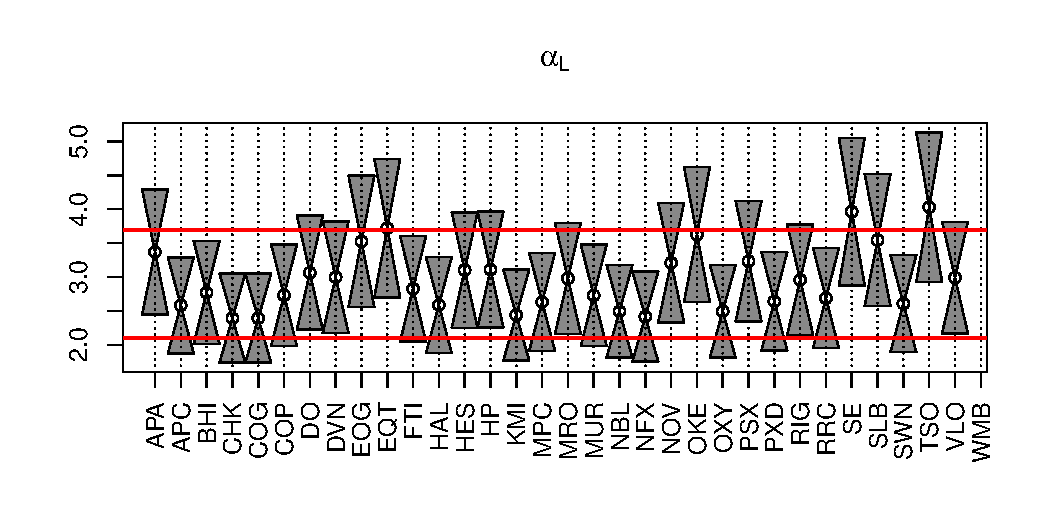
\includegraphics[width=\textwidth, trim={0, 0.8cm, 0, 2cm}, clip]
    {Energy_lower.pdf}
  \end{minipage}
  \begin{minipage}{1.0\linewidth}
    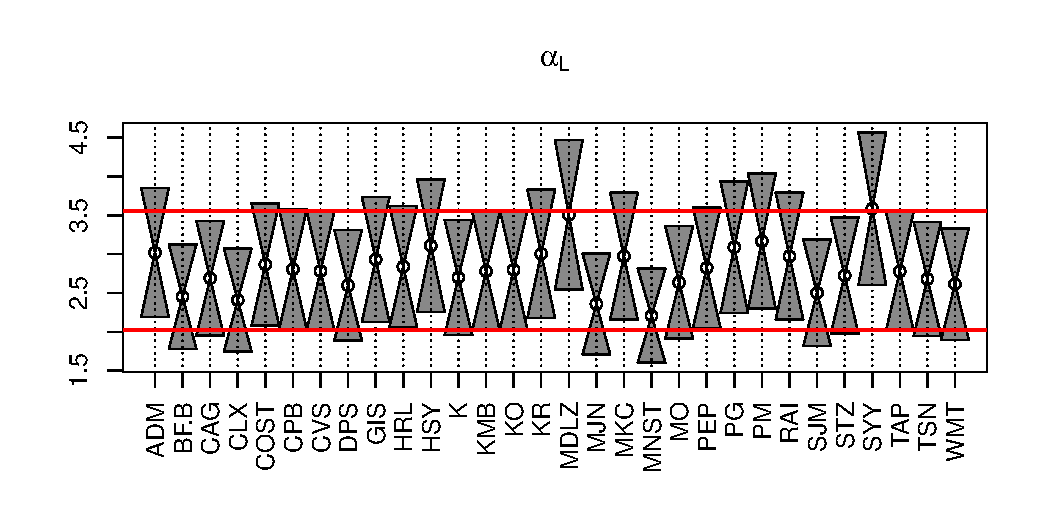
\includegraphics[width=\textwidth, trim={0, 0.8cm, 0, 2cm}, clip]
    {Consumer_Staples_lower.pdf}
  \end{minipage}
  \begin{minipage}{1.0\linewidth}
    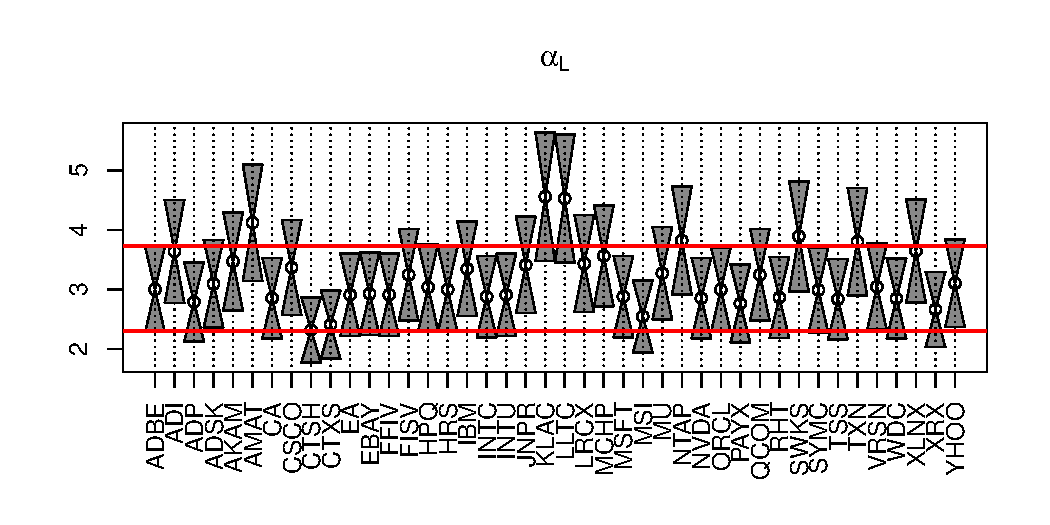
\includegraphics[width=\textwidth, trim={0, 0.8cm, 0, 2cm}, clip]
    {Information_Technology_lower.pdf}
  \end{minipage}
  \caption{\small Hill estimates $\hat \alpha_{50}$ of the lower tail indices $\alpha$ of
    daily return series in sectors of the S\&P 500
    index. The data span
    from 2010-01-01 to 2015-01-01 and comprise $n=1304$ observations.
The graphs from top to bottom correspond to the ``Energy'',
    ``Consumer Staples'' and ``Information Technology'' sectors.
    Each circle corresponds to a Hill estimate $\hat\alpha_k$; the grey
    triangles above and below it mark the 97.5\% and 2.5\% quantiles
    of its approximate normal distribution; see \eqref{eq:2} and the discussion following it for an 
interpretation.
    The lower and upper red lines mark the medians of the 2.5\% 
    and 97.5\% quantiles, respectively, evaluated from all stocks in the sector.
    The data are taken from {\it Yahoo Finance}; the labels on
    the horizontal axes are Yahoo symbols of the stocks. 
  }\label{fig:1}
\end{figure}

In Figure~\ref{fig:1} we see significant overlap of the confidence intervals of the Hill
estimates of the losses in the ``Energy'' and ``Consumer Staples''
sectors of the S\&P 500 index, as well as those of a 
large portion of losses in the ``Information Technology'' sector.
This fact indicates that the returns in each sector may 
have comparable tail indices.
\par
Hoga's \cite{hoga:2016} test about the change of extreme quantiles
may provide some further insight about how similar these tail indices are.
Different tail indices are likely to result in different
extreme quantiles. Nevertheless, changes in the extreme quantiles may also
result from changing scale parameters in the tail. Therefore  we first investigate the scale
parameters of daily stock returns in the same sectors of S\&P 500 before we apply the test.


\subsection{Hill estimates of lower-tail scale parameters}\label{sec:HillScaleEstimates}
We assume the pure Pareto model \eqref{eq:3} with scale parameter $K>0$.
Hill \cite{hill1975simple} proposed  the maximum-likelihood estimator of $K$
derived from the joint \ds\ of $k$ upper order statistics in the sample; cf.
Embrechts et al. \cite{embrechts:klueppelberg:mikosch:1997}, p.~334.
It is given by
\beao
\hat K_k = \left({k \over n}\right)^{1/\hat\alpha} X_{(n-k)}\,.
\eeao
{\blue
Using the asymptotic normality property of upper order statistics
(cf. de Haan and Ferreira~\cite{haan:ferreira:2006}, theorem 2.2.1), one can show
\begin{eqnarray*}
  \sqrt k (\hat K_k - K) &\overset{d}{\to}& N\left(
    0, \left( {K \over \alpha}  \right)^2
  \right) \\
  \sqrt k (\hat K_k^\alpha - K^\alpha) &\overset{d}{\to}& N\left(
    0, \left( {K^{2\alpha}}  \right)^2
  \right)
\end{eqnarray*}
where the tail index $\alpha$ is regarded as known. From the above
asymptotic normality property, confidence bands of the estimate of $K$
and $K^\alpha$ can be constructed. 
Estimates of $K$ of the ``Energy'', ``Consumer Staples'' and
``Information Technology'' sectors of the S\&P 500 index are computed
using this method. The results are shown in
Figure~\ref{fig:sectors_parameters}.
\begin{figure}[htb!]
  \centering
  \begin{minipage}{0.33\linewidth}
    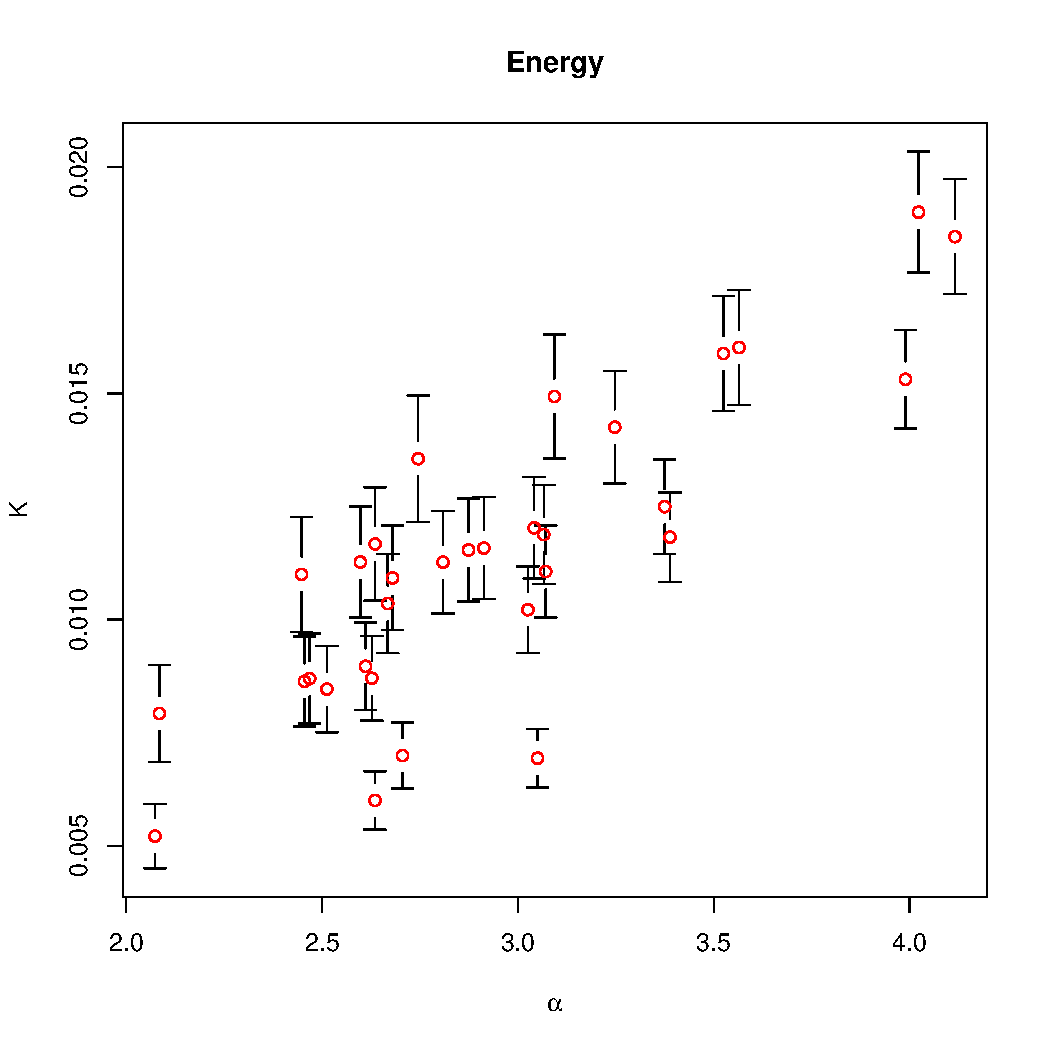
\includegraphics[width=\textwidth]
    {Energy_K.pdf}
  \end{minipage}\hfill
  \begin{minipage}{0.33\linewidth}
    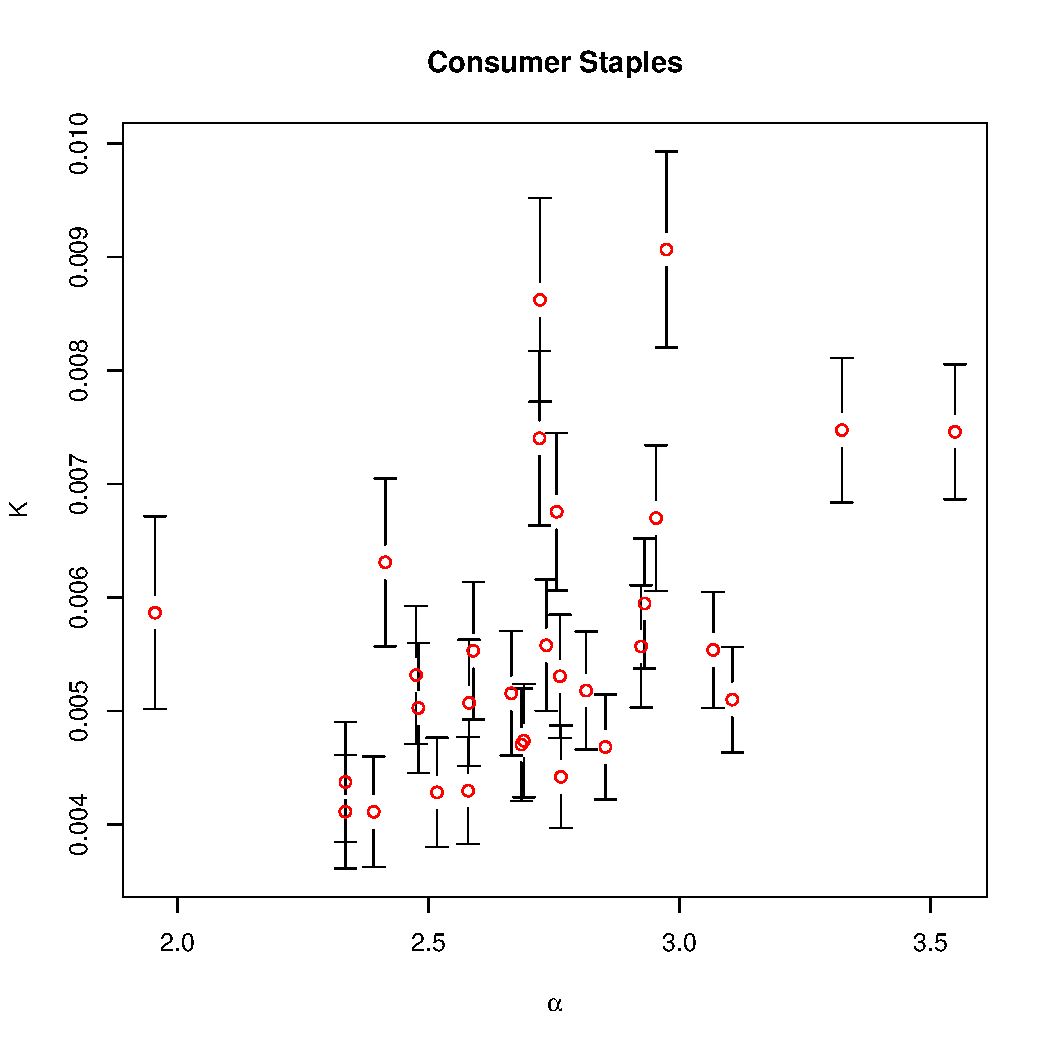
\includegraphics[width=\textwidth]
    {Consumer_Staples_K.pdf}
  \end{minipage}\hfill
  \begin{minipage}{0.33\linewidth}
    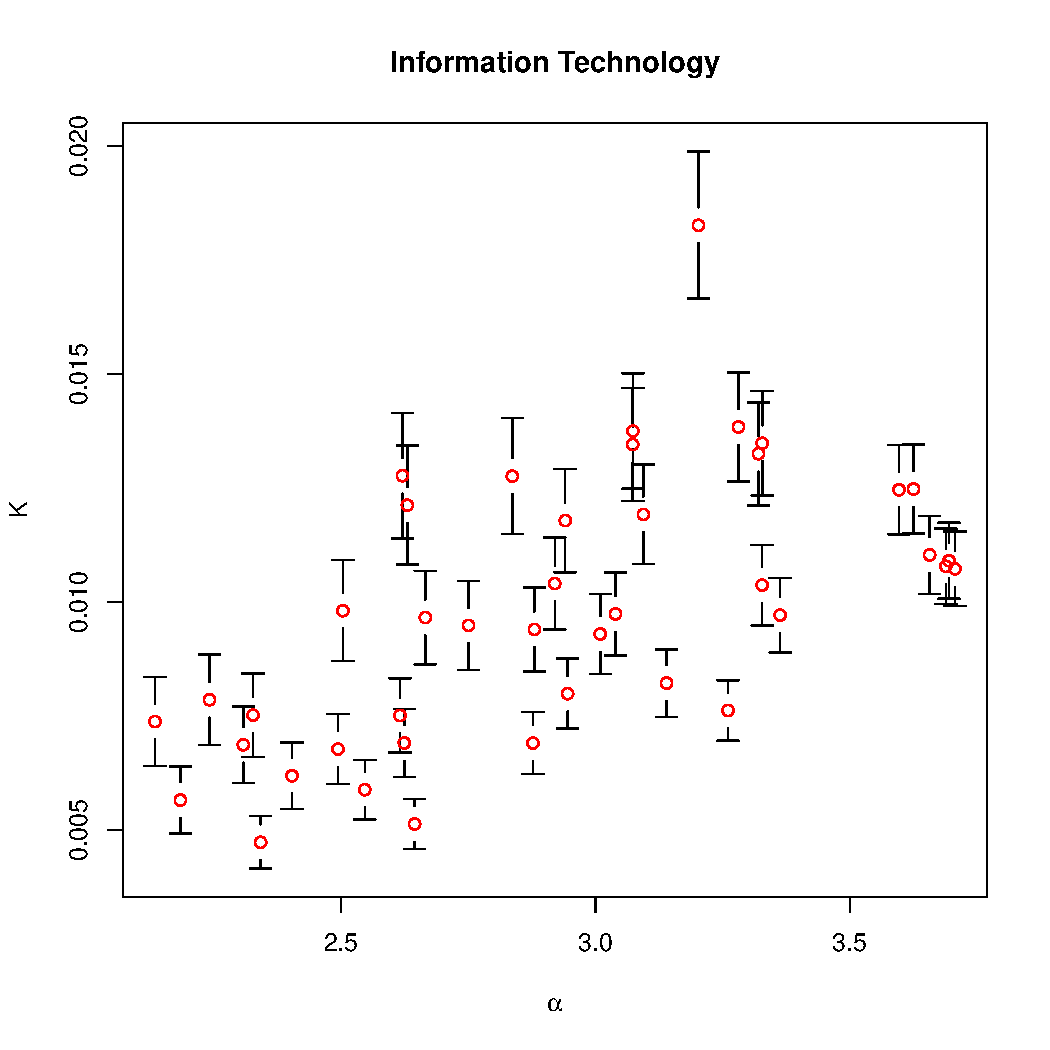
\includegraphics[width=\textwidth]
    {Information_Technology_K.pdf}
  \end{minipage}
  \begin{minipage}{0.33\linewidth}
    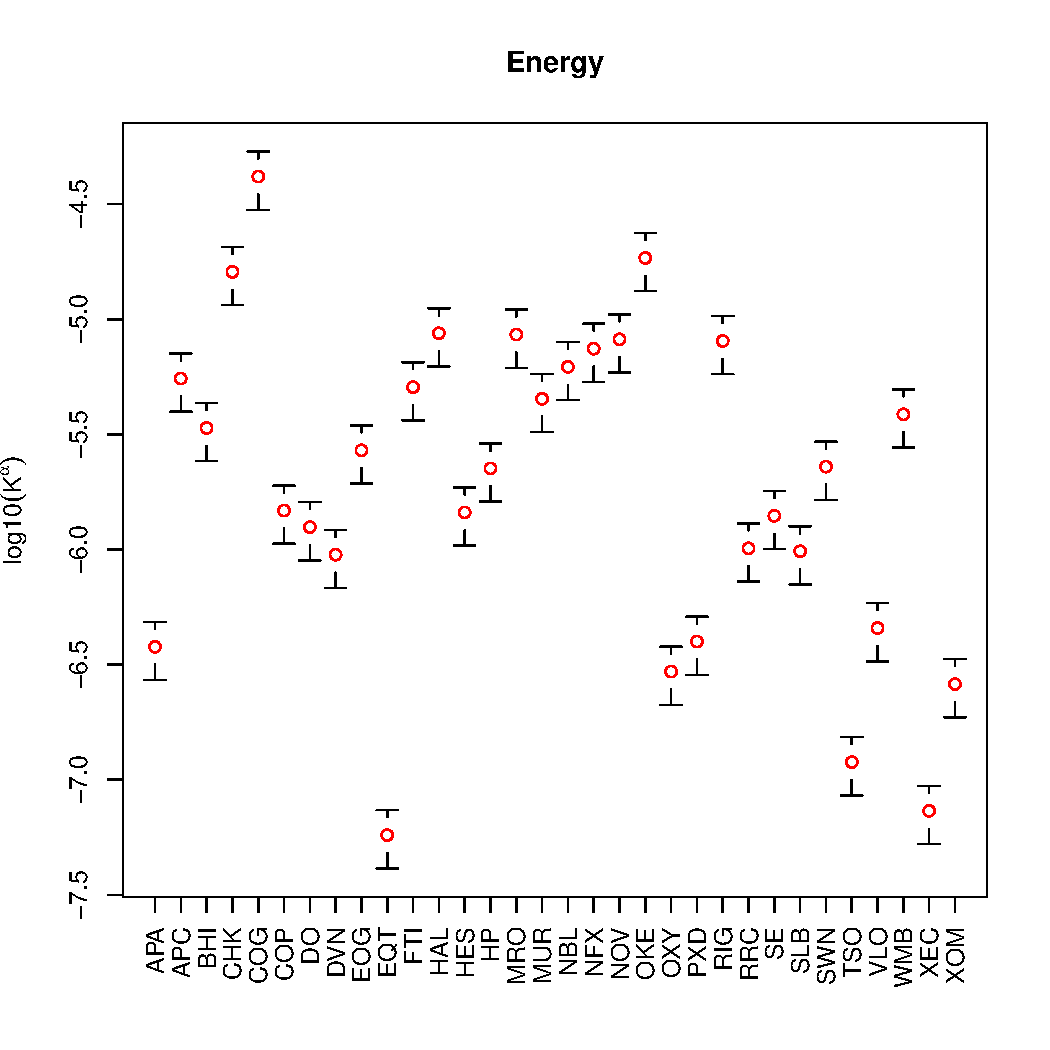
\includegraphics[width=\textwidth]
    {Energy_scale.pdf}
  \end{minipage}\hfill
  \begin{minipage}{0.33\linewidth}
    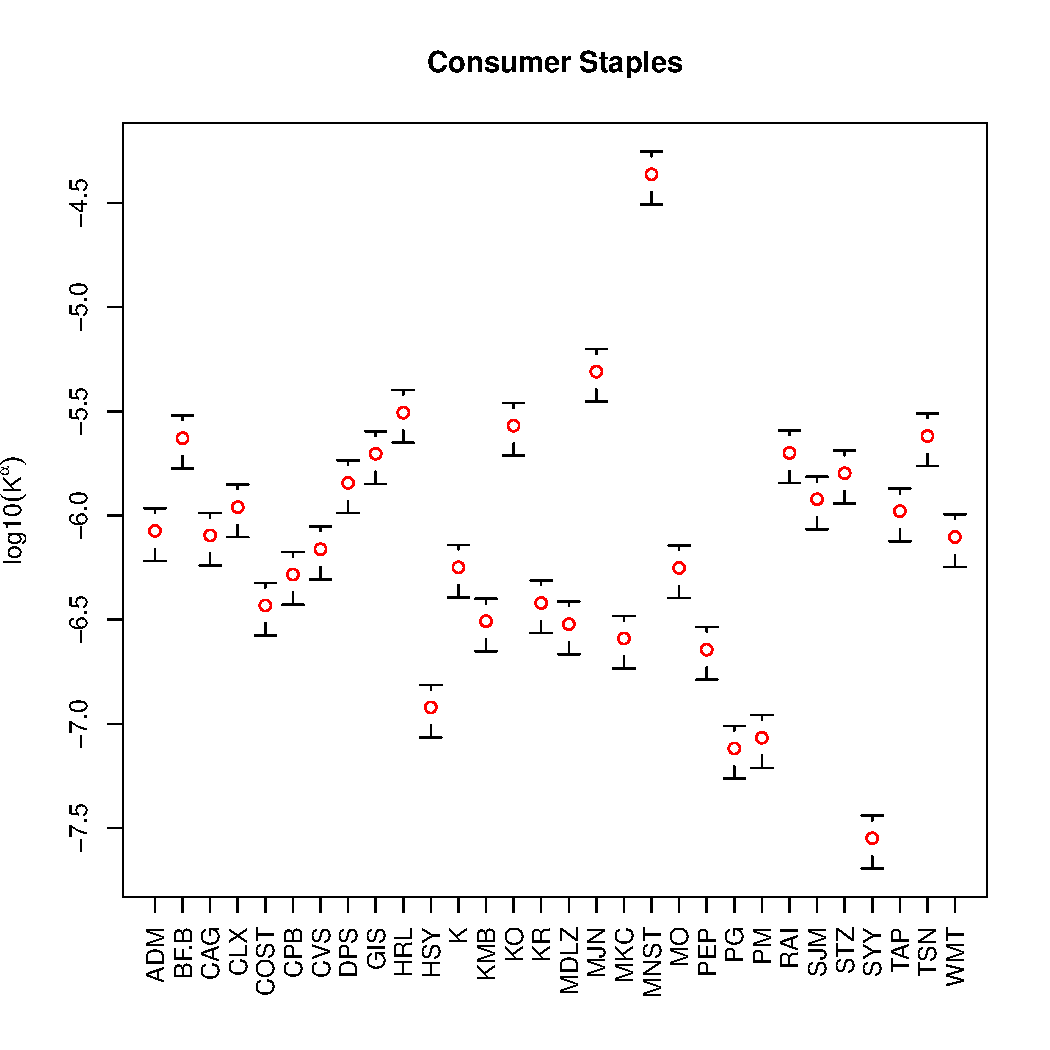
\includegraphics[width=\textwidth]
    {Consumer_Staples_scale.pdf}
  \end{minipage}\hfill
  \begin{minipage}{0.33\linewidth}
    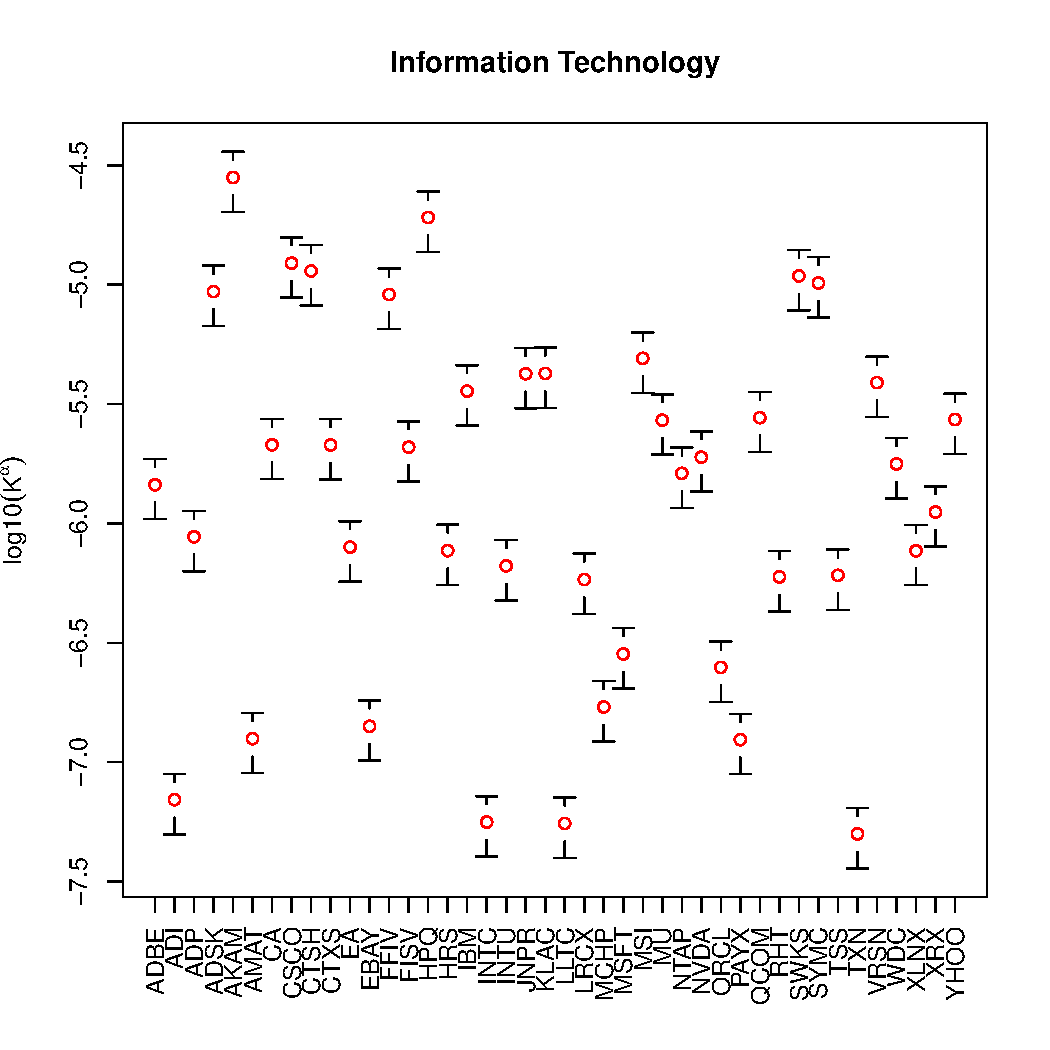
\includegraphics[width=\textwidth]
    {Information_Technology_scale.pdf}
  \end{minipage}
  \caption{\small Estimates of $K$ and $K^\alpha$ of stocks in sectors
    of the S\&P 500 index. The points are the estimated values; the bars are
    the $2\sigma$ confidence intervals. The confidence bands of the
    corresponding Hill estimates $\hat \alpha$ of these sectors are
    shown in figure~\ref{fig:1}. Note $\log_{10}(K^\alpha)$ is shown
    instead of $K^\alpha$.
  }
  \label{fig:sectors_parameters}
\end{figure}
One can see that $K$ generally takes a rather small value. For the
more volatile sectors of ``Energy'' and ``Information Technology'',
the average value of $K$ is around 0.01, while for the more stable
sector of ``Consumer Staples'', the average value is around 0.005. Due
to the smallness of $K$, mild variations of $\alpha$ would lead to
huge variations of $K^\alpha$, as shown in the 2nd column of
figure~\ref{fig:sectors_parameters}.

Secondly, one can see that the values of $\alpha$ and $K$ appear
positively correlated. This prompts Pareto tails of the return
distributions. We expain more about this in
section~\ref{sec:pareto_tail}.

Thirdly, figure~\ref{fig:sectors_parameters} shows the values of $K$
in the ``Energy'' and ``Information Technology'' sectors are on
average larger than those in the ``Consumer Staples'' sector. A larger
value of $K$ means, for a given value of $p$, i.e. a given probability
of losses, large losses are more probable. Thus one can conclude that
these two sectors are considerablly riskier than the ``Consumer
Staples'' sector. This is of course a confirmation of one's economic
instinct.

Yet another indication from figure \ref{fig:sectors_parameters} is
that, while the ``Energy'' and the ``Information Technology'' sectors
are similar in riskiness, the correlation between $\alpha$ and $K$ is
stronger in ``Energy''. As discussed in the last section, moving along
a curve of equal preference in the direction of increasing $\alpha$, $K$ also
increases. So the strong positive correlation seen in the ``Energy''
sector suggests these stocks might have very similar investor
preferences. This in turn may be attributed to stronger business
relations between the energy enterprises. While two IT companies
may provide a variety of products and services and not depend on each
other, two energy companies are more likely to depend on each other
via relations of supplier and customer or otherwise to compete with each
other if they are on the same link of the chain of energy production
and distribution.

\subsection{A test of equal tail indices based on Hill estimator}
Suppose we have two weakly dependent series $X_1, \dots, X_n \sim F_X$ and
$Y_1, \dots, Y_n \sim F_Y$. Both $F_X$ and $F_Y$ have power-law tails
with indices $\alpha_X$ and $\alpha_Y$, respectively. Assume also
$X_i$ is independent of $Y_j$ for all $1 \leq i \leq j \leq n$.
From \eqref{eq:2} one can deduce
\begin{equation}
  \label{eq:x3}
  \sqrt k
  \begin{pmatrix}
    {\hat \alpha_X - \alpha_X} \\
    {\hat \alpha_X - \alpha_X} \\
  \end{pmatrix} \overset{d}{\to}
  \begin{pmatrix}
    Z_X \\
    Z_Y
  \end{pmatrix}
  \sim
  N\left(
    0, \text{diag}(\alpha_X^2, \alpha_Y^2)
  \right)
\end{equation}
where $\hat \alpha_X$ and $\hat \alpha_Y$ are Hill estimates of
$\alpha_X$ and $\alpha_Y$. Then it follows from continuous mapping
theorem
\begin{equation}
  \label{eq:x1}
  \sqrt k [(\hat \alpha_X -\alpha_X) - (\hat \alpha_Y - \alpha_Y)]
  \overset{d}{\to}
  Z_X - Z_Y \sim N(0, \alpha_X^2 + \alpha_Y^2)
\end{equation}
The weak convergence of \eqref{eq:x1} allows one to construct a test
of the equality $\alpha_X = \alpha_Y$. As the null hypothesis, assume
$\alpha_X = \alpha_Y$. Under this hypothesis, \eqref{eq:x1} means the
test statistic $\hat \alpha_X - \hat \alpha_Y \overset{d}{\to} N(0,
\alpha_X^2 + \alpha_Y^2)$. 
We apply this test to the equities in the ``Energy'',
``Consumder Staples'' and ``Information Technology''
sectors of the S\&P 500 index. The results are shown in
\ref{fig:PairTest}.
\begin{figure}[htb!]
  \begin{minipage}{0.33\linewidth}
    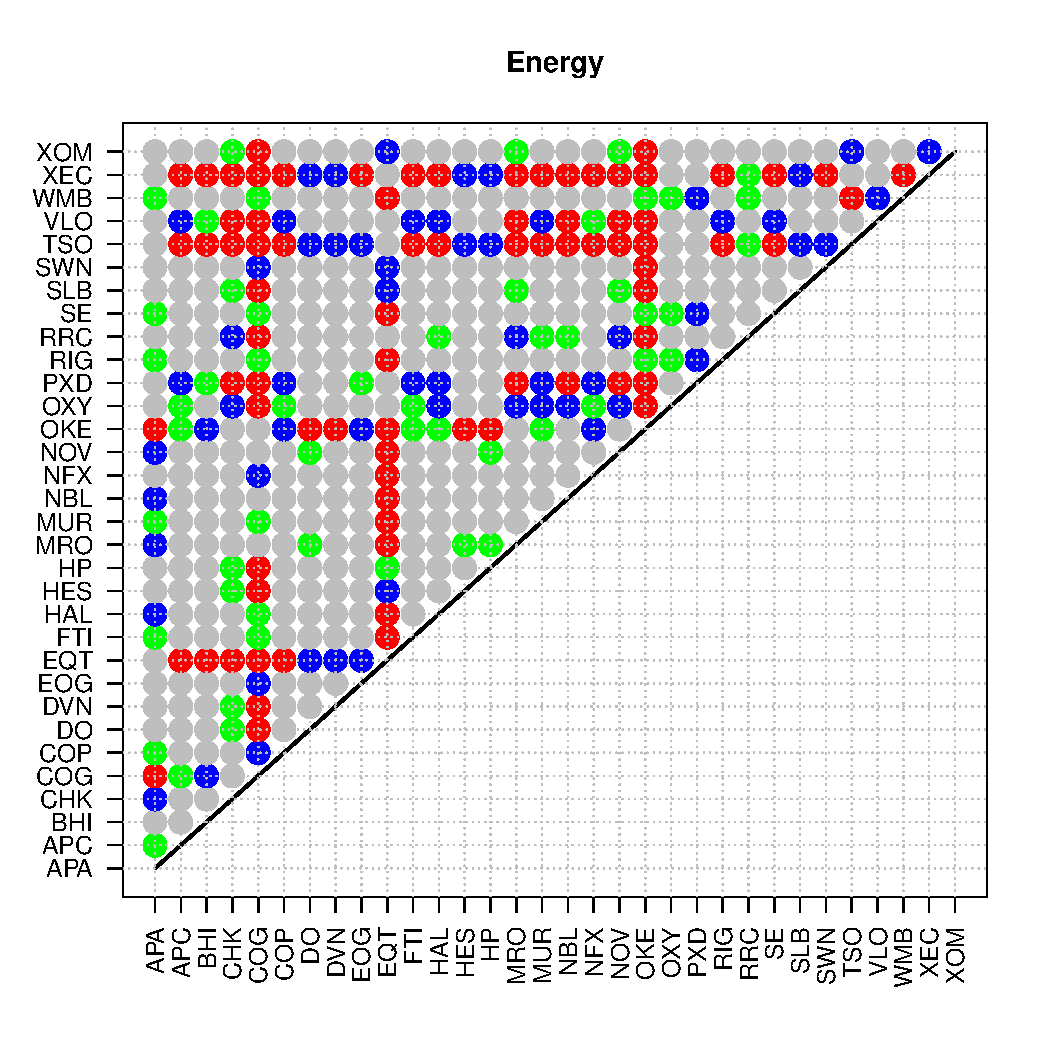
\includegraphics[
      width=\textwidth,
      trim={0.3cm, 0.8cm, 1cm, 0.6cm}, clip
    ]{HillTest_Energy.pdf}
  \end{minipage}\hfill
  \begin{minipage}{0.33\linewidth}
    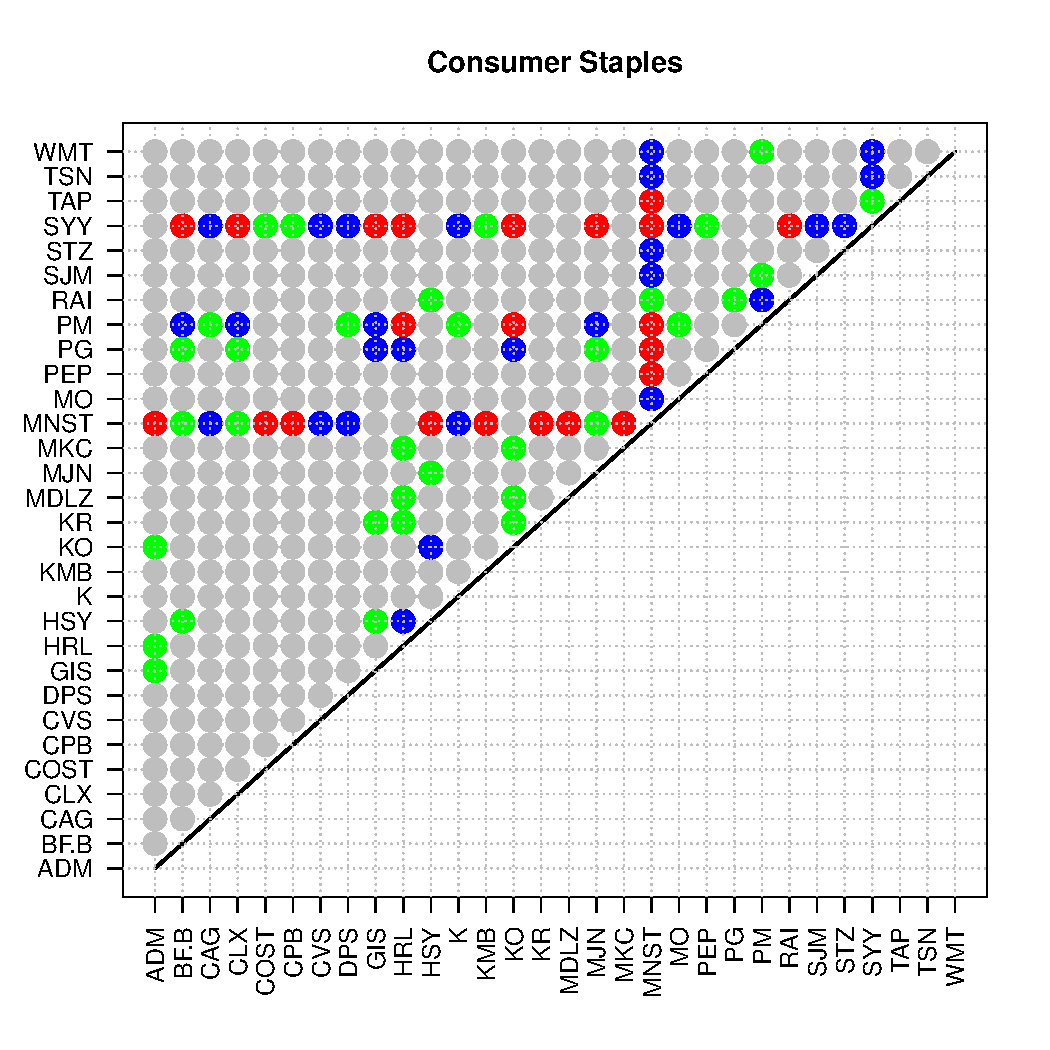
\includegraphics[
      width=\textwidth,
      trim={0.3cm, 0.8cm, 1cm, 0.6cm}, clip
    ]{HillTest_CS.pdf}
  \end{minipage}\hfill
  \begin{minipage}{0.33\linewidth}
    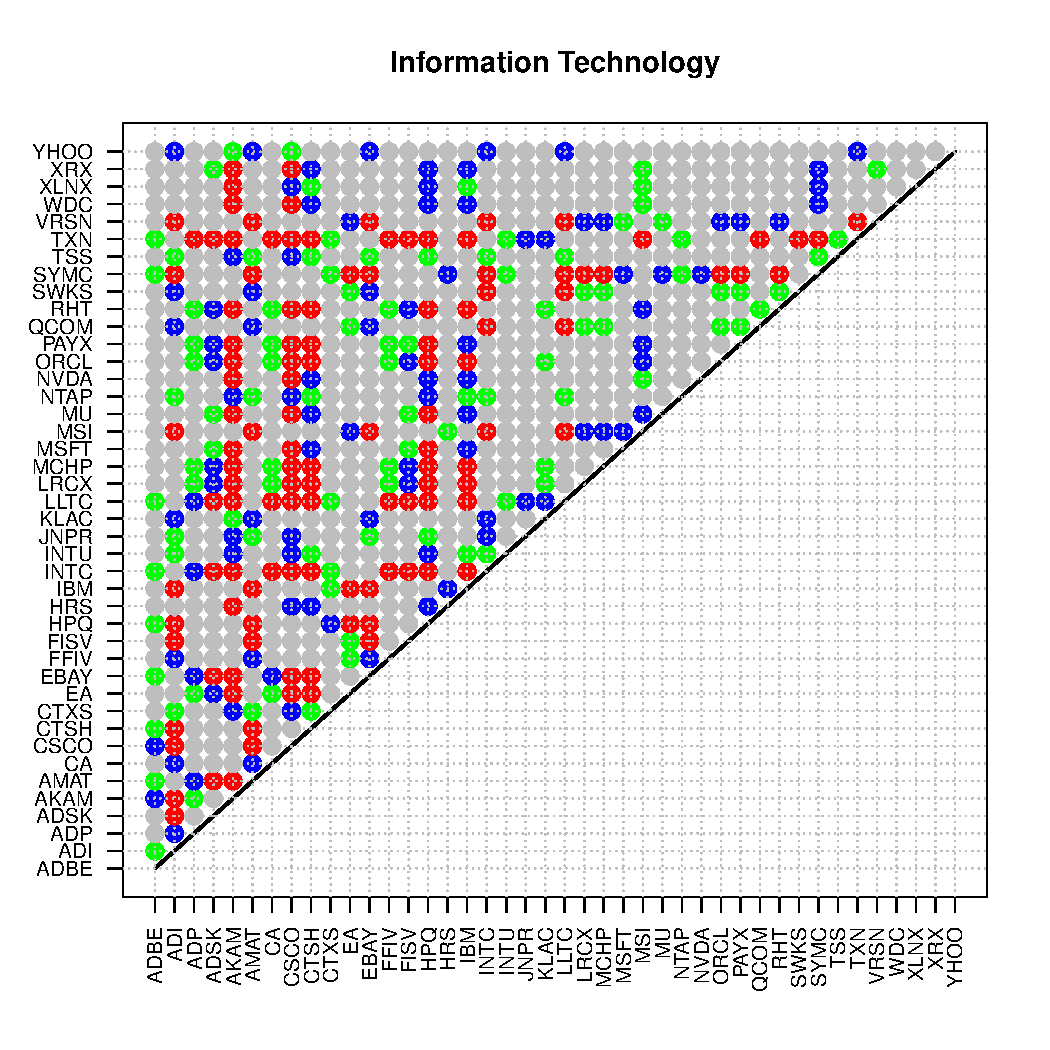
\includegraphics[
      width=\textwidth,
      trim={0.3cm, 0.8cm, 1cm, 0.6cm}, clip
    ]{HillTest_IT.pdf}
  \end{minipage}
  \begin{minipage}{0.33\linewidth}
    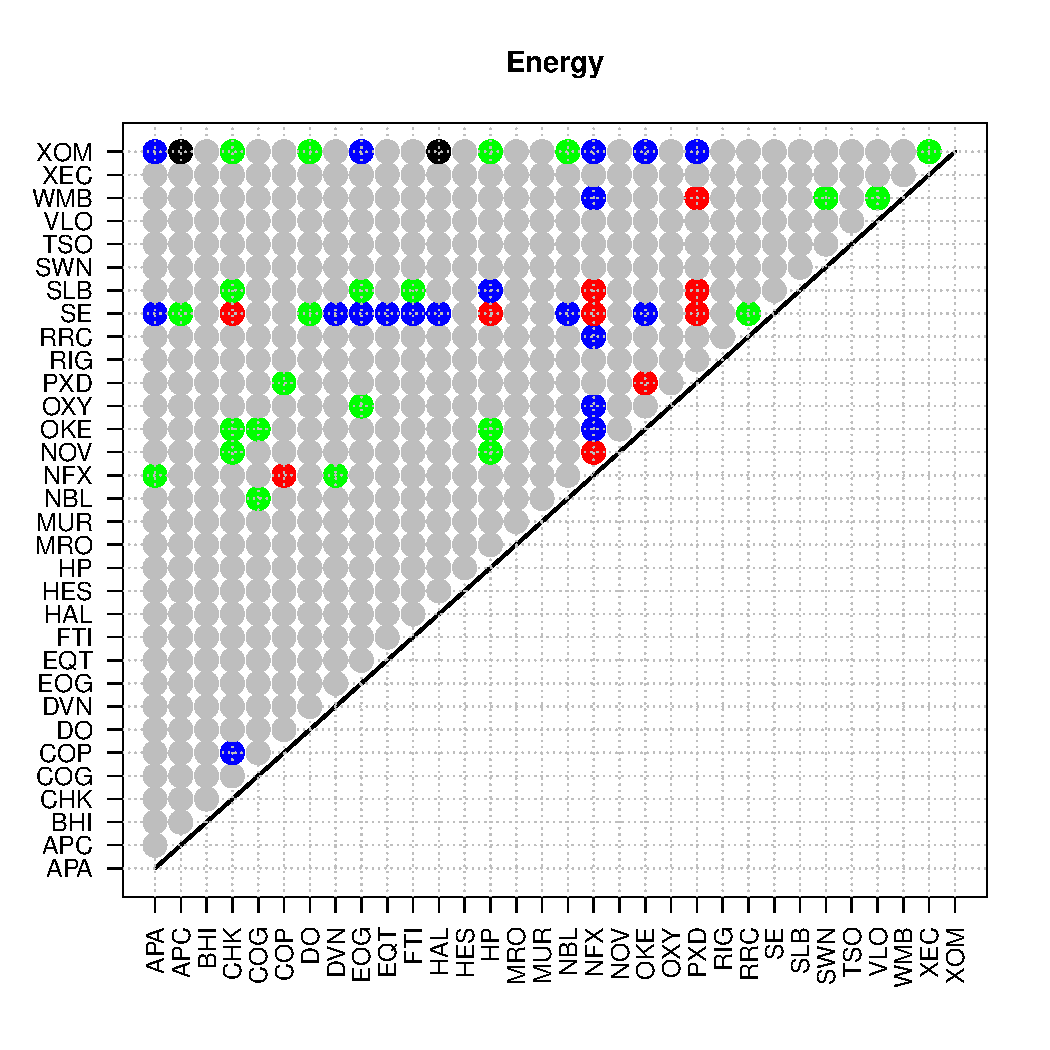
\includegraphics[
      width=\textwidth,
      trim={0.3cm, 0.8cm, 1cm, 0.6cm}, clip
    ]{Hoga_Energy_pair.pdf}
  \end{minipage}\hfill
  \begin{minipage}{0.33\linewidth}
    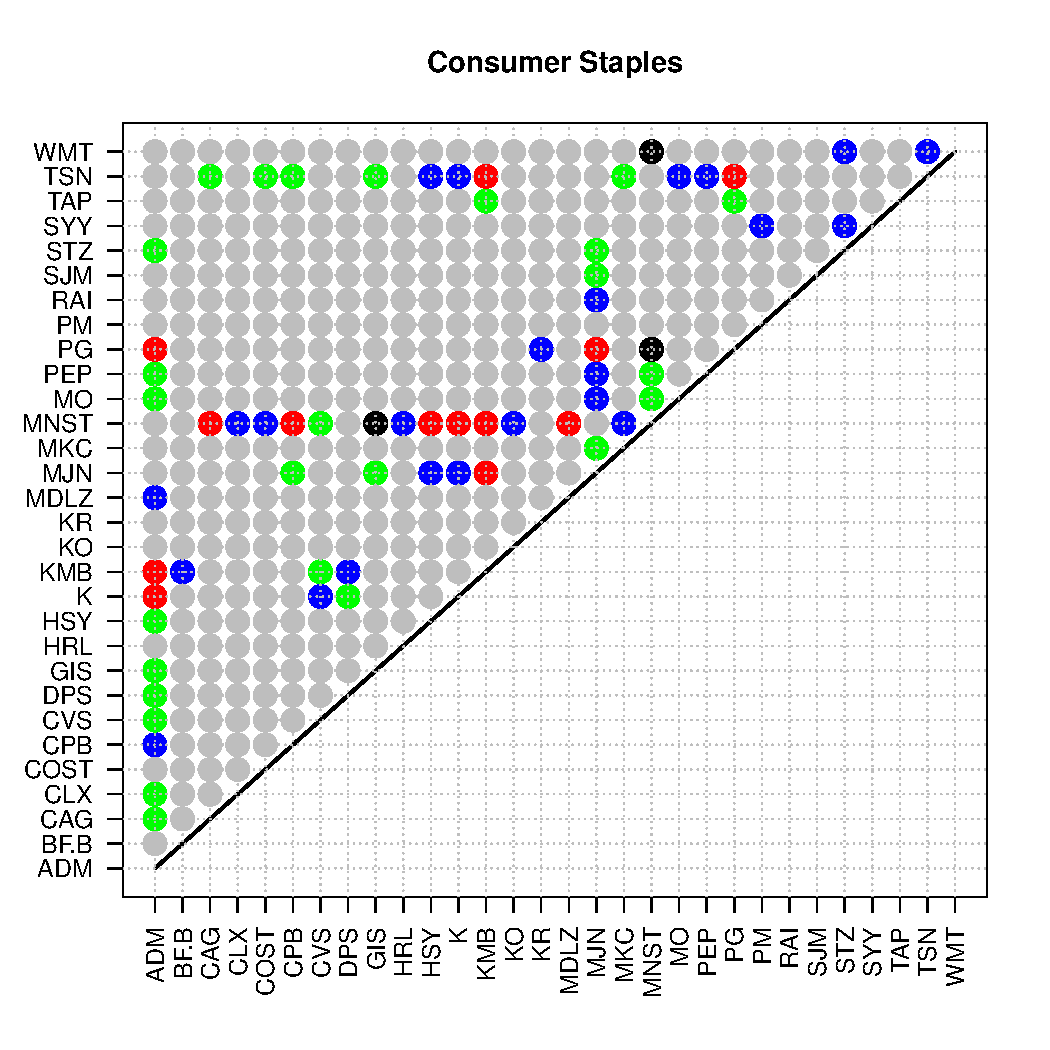
\includegraphics[
      width=\textwidth,
      trim={0.3cm, 0.8cm, 1cm, 0.6cm}, clip
    ]{Hoga_CS_pair.pdf}
  \end{minipage}\hfill
  \begin{minipage}{0.33\linewidth}
    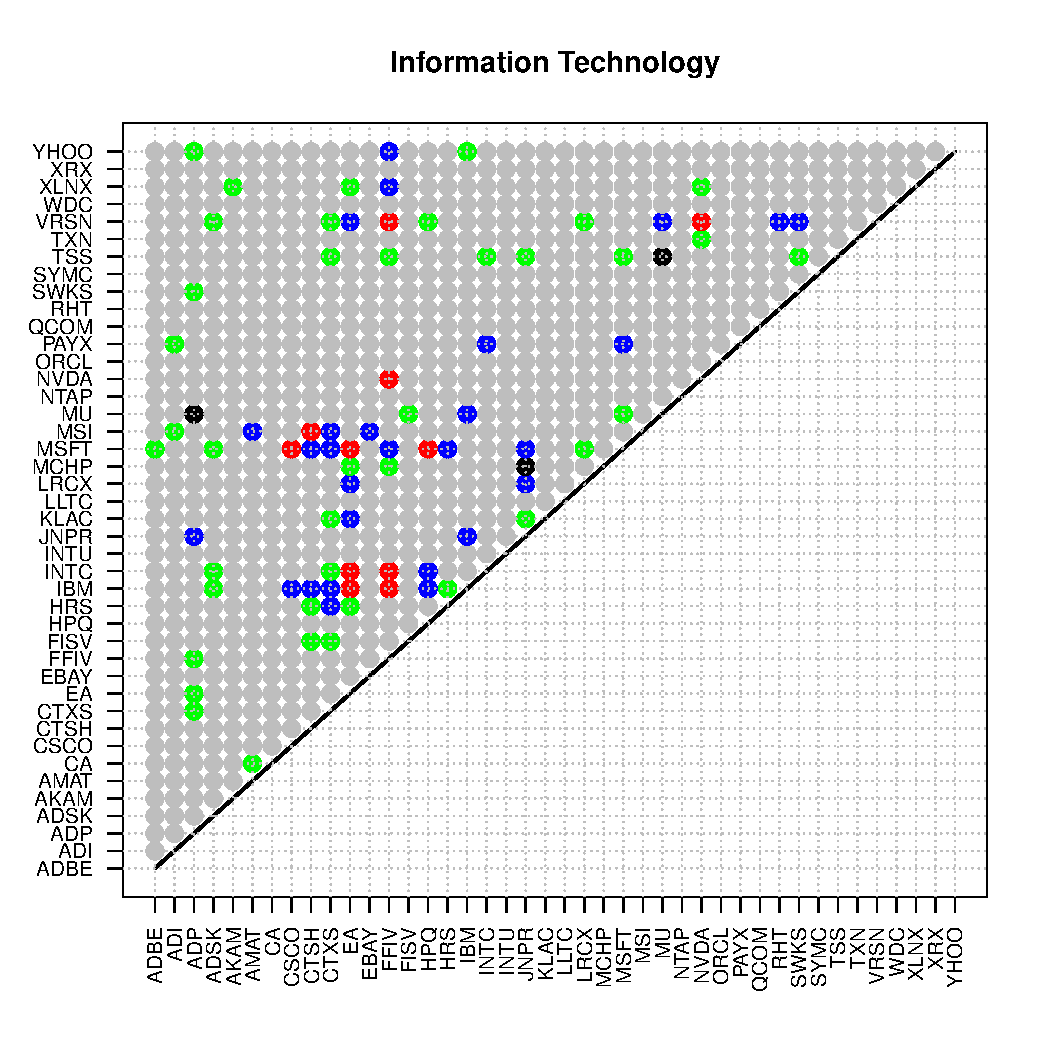
\includegraphics[
      width=\textwidth,
      trim={0.3cm, 0.8cm, 1cm, 0.6cm}, clip
    ]{Hoga_IT_pair.pdf}
  \end{minipage}
  \caption{
    {\em 1st row}: Test for changing tail index using Hill estimator based on
    concatenated series in the ``Energy'' and ``Consumer Staples''
    sectors of S\&P 500. The green, blue and red colors represent,
    respectively, the cases when the 85\%, 90\% and 95\% quantiles of
    the limit distribution of the test statistic is exceeded. 
    Grey points stand for pairs for which the test statistic is below
    the 85\% \asy\ quantile;
    {\em 2nd row:} Test for changing tail index or scale parameter
    using Hoga's test based on the same concatenated series. black points represent
    pairs for which the computation of $T_n$ fails for given precision
    requirements and time limits.
    The same number of upper-order statistics are used for both tests.
  }
  \label{fig:PairTest} 
\end{figure}
One can see from the figure that tail indices of equities in the
``Energy'' or ``Information Technology'' sectors vary more than do
their counterparts in the ``Consumer Staples'' sector, as the null
hypothesis is rejected more often for members of these two sectors.
Moreover, these figures suggest that the test based on Hill estimator
is more powerful in distinguishing differences between tail indices,
as it results in more rejections for the ``Energy'' and the
``Information Technology'' sectors than does the other test. We
argue this lack of power of the latter can be the result of slow
convergence of the distribution of its test statistic to the
asymptotic distribution. We elaborate on this in section~\ref{sec:Hoga}.

Nevertheless, one should bear in mind that the weak convergence
\eqref{eq:x3} is valid only on condition that both the $X_i$ and $Y_i$
series are independent of each other, which is generally untrue for
two return series in the same market.
}


\subsection{Tests for a change in the extreme tail}\label{sec:Hoga}
To the best of our knowledge, there do not exist published statistical
tests for comparing the tail indices or scale parameters of two or
more dependent \ts\ in a direct way. In addition to the test described
in the previous section, we borrow a test from
a recent paper by Hoga \cite{hoga:2016}. This test has been developed
for a different kind of problem. Given a strictly stationary
\ts\ $X_1,\ldots,X_n$ with a marginal \ds\ $F$ with right power-law
tail, the goal is to test whether there is a structural break of the
{\em extreme quantiles} $F^{-1}(1-p)$ for values $p$ very close to
zero. If the tail index {\em or} the scale parameter in a \ds\ of type
\eqref{eq:3} change inside a sample, then it is likely that the
extreme quantiles change as well. We will test for a change of tail
index or scale parameter in this indirect way.
\par
The null hypothesis of the test in \cite{hoga:2016} is that there is no change of the extreme quantiles $F^{-1}(1-p)$ 
for $p=p_n\to 0$ in any subsample with indices
$t\in (n\,t_0,n(1-t_0))$ where $t_0$ is a fixed number in $(0,0.5)$. Writing $\hat x_p(a,b)$ for an estimator of the extreme $(1-p)$-quantile 
based on the subsample with indices $t\in (na,nb)$, the test statistic is given by
\beam\label{eq:4}
T_n = \sup_{s \in [t_0, 1 - t_0]}
  \dfrac{  \big[s (1 - s) \log \big(\hat x_p(0, s)/\hat x_p(s, 1)\big)
    \big]^2}{
    \int_{t_0}^s\big[r \log \big( \hat x_p(0, r)/\hat x_p(0, s)
      \big)
    \big]^2 dr
    +
    \int_{s}^{1 - t_0}
    \big[
      (1 - r) \log \big(
      \hat x_p(r, 1)/
      \hat x_p(s, 1)
      \big)
    \big]^2 dr}\nonumber\\
\eeam
Under the null hypothesis, $(T_n)$ converges to a complicated \fct al of \BM\ on $[0,1]$; the \asy\ quantiles need to be 
evaluated by simulation.  
\par
When applied to our problem we would like to test 
whether there is a change of the tail index {\em or} scale parameter in \eqref{eq:3} in each of the S\&P 500 
series in the distinct sectors. We also  want to get some indication about a possible change of tail index or
scale parameter from one series to another within a given sector. For this reason, we choose any pair of series
within a sector and concatenate each of the paired series. Then we run the test on the concatenated series.
Of course, despite the fact that we test changes of tail index or scale parameter 
{\em in a very indirect way} -- there may be many other reasons for the change of extreme quantiles in a sample -- 
we also concatenate two rather distinct series. Even if we assume that the two series come from related models
(such as GARCH), the parameters of these models will in general not be the same. Moreover, the concatenation
of two strictly stationary \ts\ is in general not strictly stationary. Therefore we have to be careful
with interpretations of the results of the tests.
\par 
In Figure~\ref{fig:Hoga_Single} we show the values of the test statistic $T_n$ (horizontal bars)
for $t_0=0.1$ and daily return series of stock in the ``Energy'' and ``Consumer Staples'' sectors of the S\&P
500 index. The ``null hypothesis'' is that the tail index and scale parameter remain the
same througout the selected period of time. For most stocks, the hypothesis cannot be rejected even at the 85\% level.
This fact may be an indication that the \ds\ inside a series is rather homogeneous.
Alternatively, it may show that the power of the test is very low. A possible reason for this suspicion is that the \con\ rate
of $(T_n)$ to its limit is very slow, i.e., the \asy\ \ds\ is not representative for the \ds\ of $T_n$ for the chosen $n$; for some
simulation evidence, see below.
\par
To check whether any two series share the same tail index and scale parameter we concatenate
any two series and apply the aforementioned test on the concatenated series. For the ``Energy'' and the
``Consumer Staples'' sector we summarize the results in Figure~\ref{fig:PairTest}.
These graphs show that the ``null
hypothesis'' of an equal tail index and scale parameter is rejected for more pairs in the
``Energy'' sector than it is for those in the ``Consumer Staples''
sector. This suggests that lower tail indices of stocks in the
``Energy'' sector are more spread out than those of the ``Consumer
Staples'' sector. Also observe that while 3 stocks, say A, B and C, test in favor of
the relations $\alpha_A = \alpha_B, \alpha_A \neq \alpha_C$, it often
happens that another test on B and C is supportive of $\alpha_B = \alpha_C$. Again,
this is due to the limited power of the test. Based
on such results, one may guess that $\alpha_B$ lies between $\alpha_A$ and
$\alpha_C$. The test is unable to recognize the smaller differences
between $\alpha_A, \alpha_B$ on one hand and between $\alpha_B, \alpha_C$ on the other hand.



\begin{figure}[htb!]
  \begin{minipage}{0.5\linewidth}
    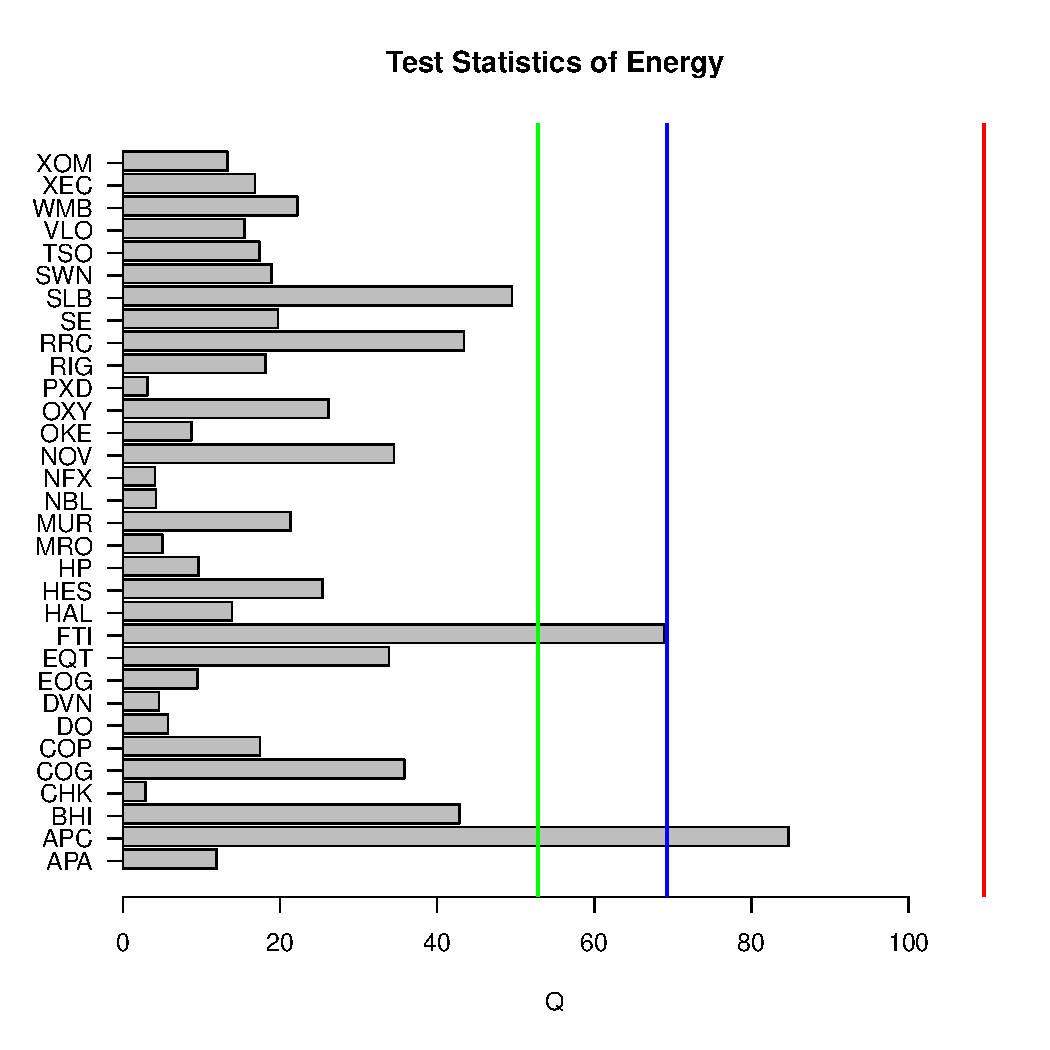
\includegraphics[width=\textwidth]
    {Hoga_Energy_Single.pdf}
  \end{minipage}\hfill
  \begin{minipage}{0.5\linewidth}
    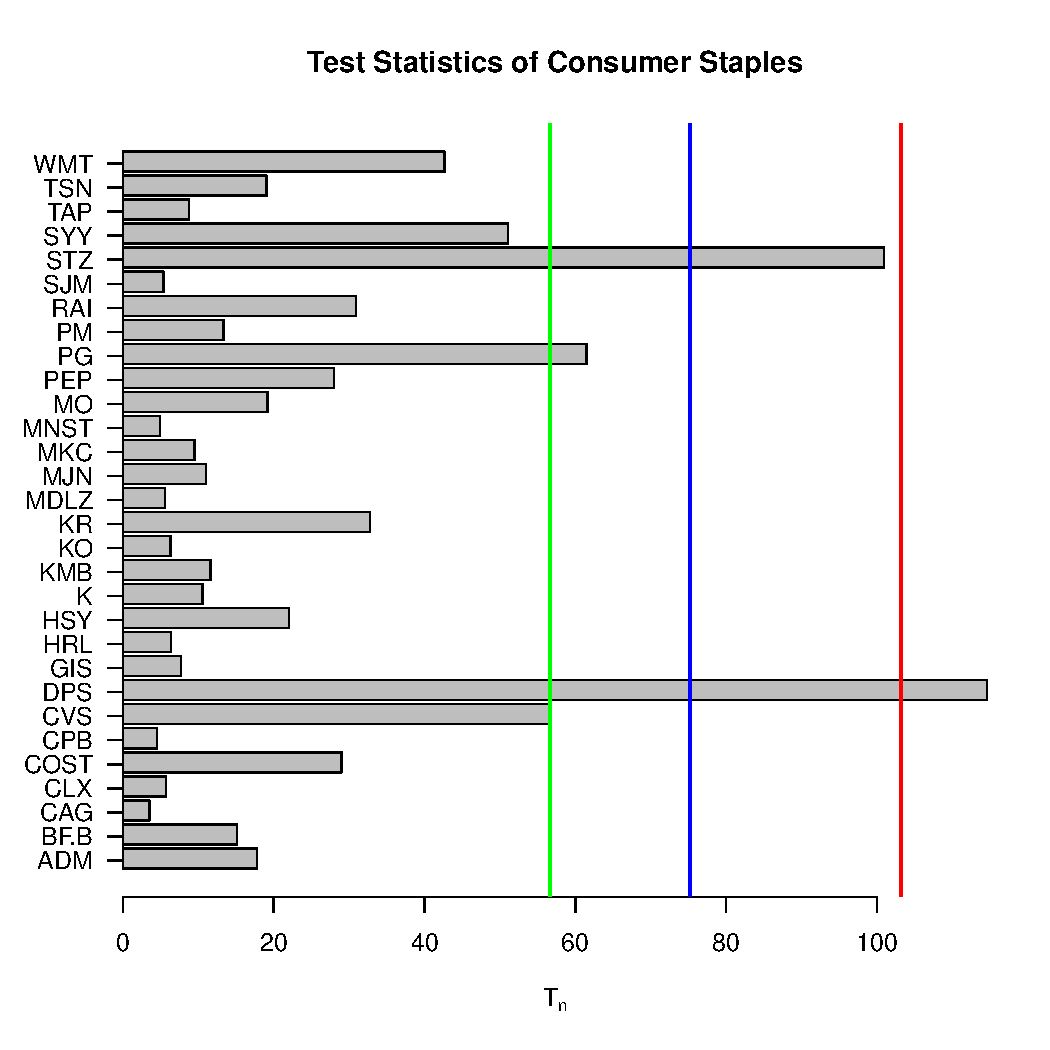
\includegraphics[width=\textwidth]
    {Hoga_CS_Single.pdf}
  \end{minipage}
  \caption{Test statistic $T_n$ from \eqref{eq:4} for the  stocks in the ``Energy'' and
    ``Consumer Staples'' sectors of S\&P 500. The green, blue and red
    lines correspond to the 85\%, 90\% and 95\% quantiles of the limit \ds\ of $T_n$.  They are derived
by simulations from the limit \ds .}
  \label{fig:Hoga_Single}
\end{figure}


% \begin{figure}[htb!]
%   \begin{minipage}{0.5\linewidth}
%     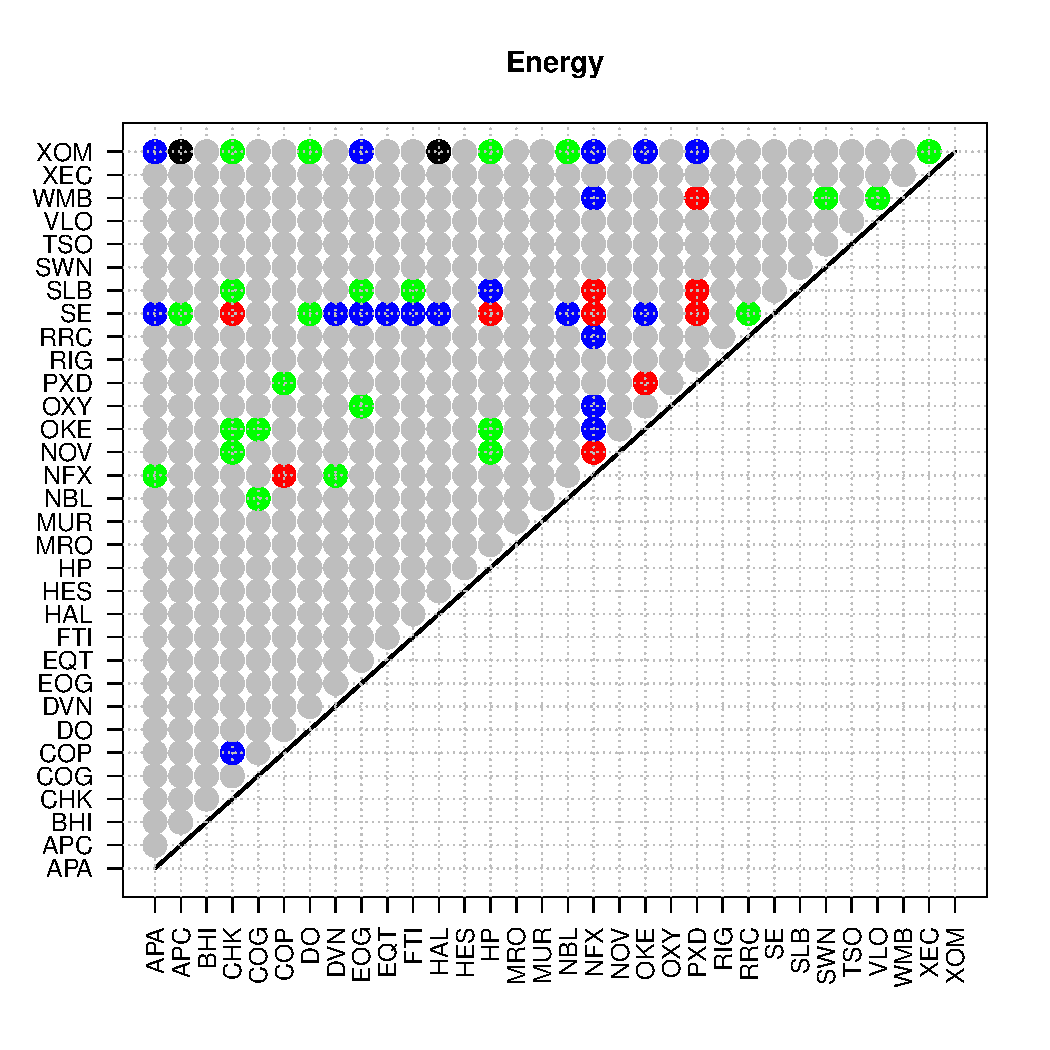
\includegraphics[
%       width=\textwidth,
%       trim={0.3cm, 1cm, 1cm, 1cm}, clip
%     ]{Hoga_Energy_pair.pdf}
%   \end{minipage}\hfill
%   \begin{minipage}{0.5\linewidth}
%     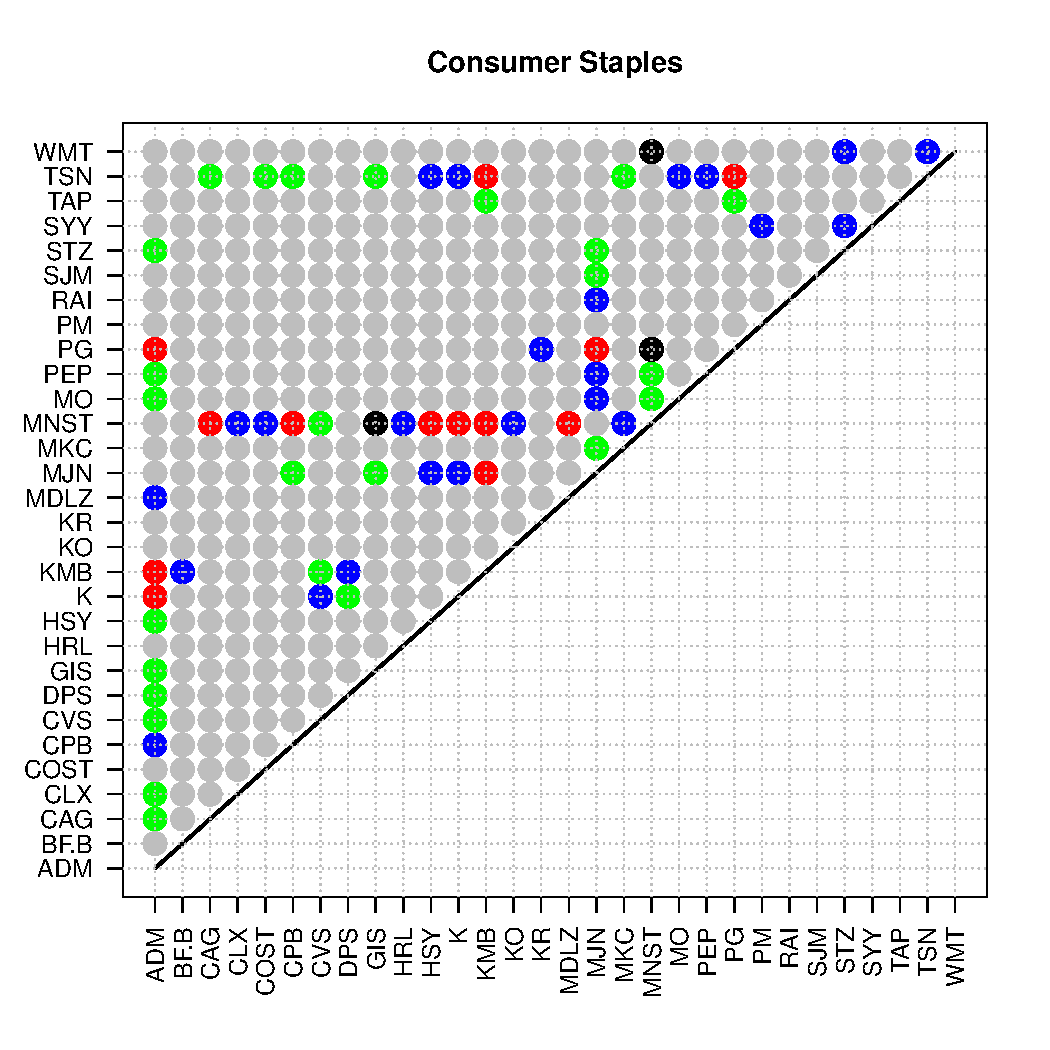
\includegraphics[
%       width=\textwidth,
%       trim={0.3cm, 1cm, 1cm, 1cm}, clip
%     ]{Hoga_CS_pair.pdf}
%   \end{minipage}
%   \caption{{\red check the symbols on the axes. Some are too long.} Test for changing tail index or scale parameter based on concatenated series in the ``Energy'' and
%     ``Consumer Staples'' sectors of
%     S\&P 500. The green, blue and red colors represent, respectively, the cases when  
%     the 85\%, 90\% and 95\% quantiles of the limit distribution of $T_n$ is exceeded.
%     Grey points stand for pairs for which $T_n$ is below
%     the 85\% \asy\ quantile;
%     black points represent pairs for which
%     the computation of $T_n$ fails for given precision
%     requirements and time limits.}
%   \label{fig:Hoga_pair}
% \end{figure}



\par
To get an idea about the power of the test we run it on a
sample concatenated from two independent iid samples of the same size
$n=1304$ as the S\&P 500 series. Both pieces are $t$-distributed with
distinct degrees of freedom. The results are shown in
Figure~\ref{fig:t_sim_pair}: the power of the test is the smaller the
larger the minimum tail index in the concatenated pair.
\begin{figure}[htb!]
  \begin{minipage}{0.5\linewidth}
    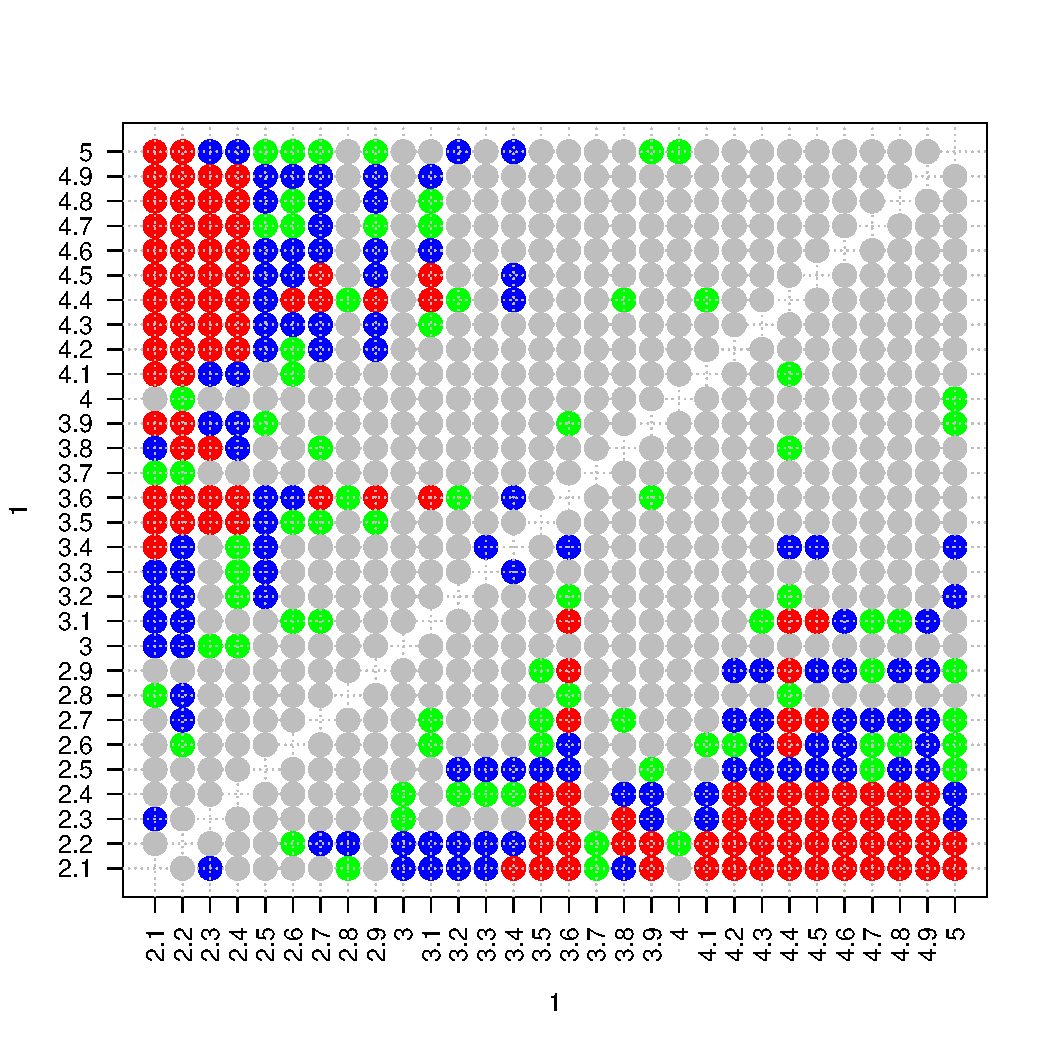
\includegraphics[width=\textwidth]{t_sim_pair.pdf}
  \end{minipage}\hfill
  \begin{minipage}{0.5\linewidth}
    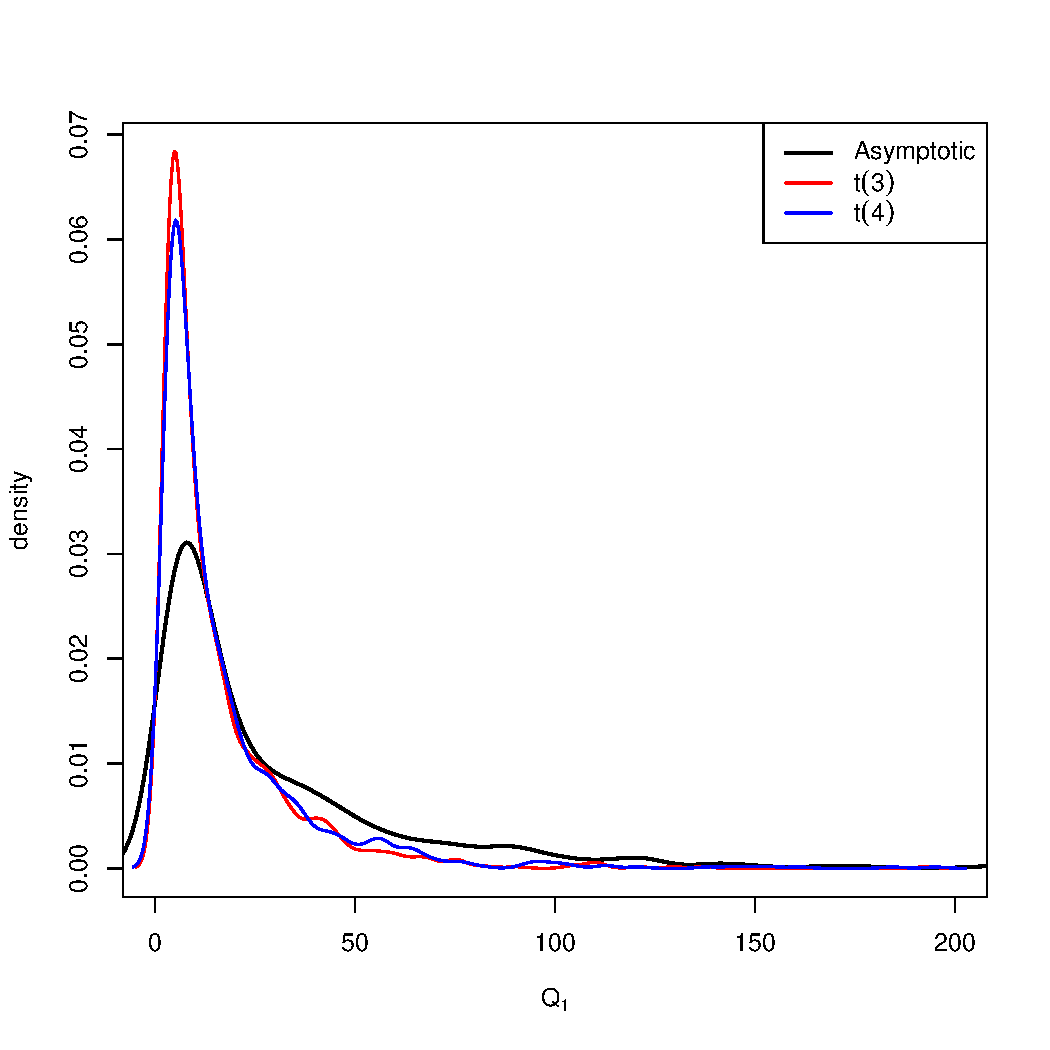
\includegraphics[width=\textwidth]{Hoga_AsymptoticDistribution.pdf}
  \end{minipage}
  \caption{
    {\em Left}: Test  of concatenated $t$-samples with different
    degrees of freedom. Numbers on the axes are the degrees of freedom
    in the subsamples. For an interpretation of the colored bullets,
    see Figure~\ref{fig:PairTest}. The graph shows the limited power
    of the test. In particular, if both degrees of freedom are
    relatively large it loses the capablity of distinguishing the \ds\ .
    {\em Right}: Comparison of the \asy\ distribution of the test statistic
    $T_n$ in \eqref{eq:4} under the null hypothesis and the \ds\ of
    $T_n$ for $n=1304$ iid $t$-distributed $X_t$ with 3 and 4 degrees
    of freedom.
  }
  \label{fig:t_sim_pair}
\end{figure}

\par
A major problem in this test is the \asy\ distribution of the test statistic under the
null hypothesis.  The rate at which the finite-sample distribution tends to its limit is not known.
To find out about this problem we compared the \ds s of $T_n$ 
with $n=1304$ for $t$-distributed $X_t$ with  3 and 4 degrees of freedom and the limit \ds\ of $T_n$.
The estimated density functions are shown in on the right of Figure~\ref{fig:t_sim_pair}.
As seen in the graph, the asymptotic distribution assigns
significantly more mass to the tail than the \ds s of $T_n$ do. For
comparison, we list a few quantiles of these \ds s in
Table~\ref{tab:HogaAsymptotic}, showing major differences between the
\asy\ and finite-sample \ds s.
\begin{table}[htb!]
  \centering
  \begin{tabular}{l|c|c|c|r}
    & \multicolumn{4}{c}{Quantiles} \\[2mm]
    \hline
    Distribution of $X_t$& 80\% & 85\% & 90\% & 95\% \\
    \hline
    Asymptotic & 47.48 & 59.61 & 78.90 & 113.12 \\
    t(3)  & 23.30 & 28.27 & 35.04 & 46.75 \\
    t(4)  & 25.76 & 31.13 & 38.81 & 56.32\\[2mm]
  \end{tabular}
  \caption{Quantiles of the test statistic $T_n$ for $n=1304$ $t$-distributed samples with 3 and 4 degrees of freedom as well
as the corresponding quantiles for the limiting \ds\ of $T_n$. In particular, there are huge differences between the three \ds s  
for the higher quantiles. 
    }
  \label{tab:HogaAsymptotic}
\end{table}

\newpage
\section{Some theoretical arguments for equality of tail indices}\setcounter{equation}{0}\label{sec:2}
\subsection{Multivariate GARCH models whose components have  equal tail indices}\label{subsec:garch}
Among the models for returns the generalized autoregressive conditionally heteroscedastic (GARCH) model
is certainly most popular because it is parsimonious, captures various of the stylized facts of real return data
and can also be modified in various directions to capture specific behavior of \ts\ such a asymmetry, skewness, long memory; 
see for example Andersen et al. \cite{andersen:davis:kreiss:mikosch:2009}, Part 1, for a collection of results
on GARCH-type models.
The original  {\em univariate} GARCH model of Bollerslev \cite{bollerslev:1986} is a \sv\ model of the type $X_t=\sigma_t\,Z_t$, where 
$(Z_t)$ is an iid mean-zero unit-variance \seq . In the simple case of a \garch\ the {\em squared volatility} satisfies the {\em \sre} 
\beam\label{eq:5}
\sigma_t^2= \alpha_0+\alpha_1 X_{t-1}^2+\beta_1\sigma_{t-1}^2=\alpha_0+(\alpha_1Z_{t-1}^2+\beta_1)\sigma_{t-1}^2\,,\quad t\in\bbz\,.
\eeam
Here $\alpha_0>0$, $\alpha_1,\beta_1$ are non-negative constants. For suitable choices of $\alpha_1,\beta_1$ the equation \eqref{eq:5}
can be solved and the solution $(\sigma_t^2)$ constitutes a strictly stationary \seq , implying that $(X_t)$ 
is strictly stationary itself. A remarkable property of the process $(\sigma_t)$ is that it has a power-law tail 
of the form
\beam\label{eq:6}
\P(\sigma_t>x)\sim c\,x^{-\alpha}\,,\qquad \xto\,,
\eeam
for some positive $c>0$ and a positive tail index $\alpha$ being the unique solution of the equation 
$\E [(\alpha_1 Z_1^2+\beta_1)^{\alpha/2}]=1$
provided the latter soluton exists and some mild assumptions on the \ds\ of $Z_t$ hold. This result
follows by an application of the Kesten-Goldie theorem; see Kesten \cite{kesten:1973}, Goldie \cite{goldie:1991}, cf. 
Buraczewski et al. \cite{buraczewski:damek:mikosch:2016}. The latter result ensures power-law tails  for
the strictly stationary  solution $(Y_t)$ to the \sre\ 
\beam\label{eq:7}
Y_t= A_t\,Y_{t-1}+B_t\,,\qquad t\in\bbz\,,
\eeam
for an iid \seq\ of pairs $(A_t,B_t)$, $t\in\bbz$, with non-negative components satisfying $\E [A_1^\alpha]=1$.  
In the model \eqref{eq:5} we can choose $Y_t=\sigma_t^2$, $A_t=\alpha_1\,Z_{t-1}^2$ and $B_t=\alpha_0$ to achieve
\eqref{eq:6}. In turn, by an application of Breiman's lemma (see \cite{buraczewski:damek:mikosch:2016})
it follows that
\beao
\P(\pm X_t>x)\sim \E[(Z_t)_\pm^\alpha]\,\P(\sigma_t>x)\,,\qquad \xto\,, 
\eeao
implying power-laws for the right and left tails of $X_t$ caused by the power-law tail of $\sigma_t$.
A GARCH process of the order $(p,q)$ can be embedded in a multivariate equation of the type \eqref{eq:7},
where $(\bfA_t)$ are iid random matrices and $\bfB=\bfB_t$ is a constant vector. Again, the Kesten theory \cite{kesten:1973}
applies, implying that the marginal and \fidi s of the GARCH process are \regvary\ with a positive index $\alpha$.
We refrain from explaining the notion of multivariate \regvar\ which is needed in this context. For further details,
see Buraczewski et al. \cite{buraczewski:damek:mikosch:2016} where the Kesten theorem and \regvar\ of GARCH processes
are explained in detail.
\par
There exist various extensions of the univariate GARCH
model to the multivariate case. For the sake of argument, we stick here to the 
{\em constant conditional correlation} (CCC) model of Bollerslev
\cite{bollerslev:1990} and Jeantheau \cite{jeantheau:1998}, and we only consider a special bivariate case.
It is the model 
\beao\bfX_t=
\left(\barr{l}X_{1,t}\\
X_{2,t}\earr\right)= \left(\barr{ll}\sigma_{1,t}& 0\\
0&\sigma_{2,t}\earr\right)\,\left(\barr{l}Z_{1,t}\\Z_{2,t}\earr\right)=\Sigma_t\,\bfZ_t\,,\qquad t\in\bbz\,.
\eeao
Thus both return components $X_{i,t}$ have the form of a univariate \sv\ model $X_{i,t}=\sigma_{i,t}Z_{i,t}$ 
with non-negative volatility $\sigma_{i,t}$ and an iid bivariate noise \seq\ $(\bfZ_t)$ with zero mean and unite variance components.
We also have the specification
\beam\label{eq:8}
\bfY_t=\left(\barr{l}\sigma^2_{1,t}  \\  
\sigma^2_{2,t}\earr
\right)
&=& \left(
\barr{l}\alpha_{01}  \\\alpha_{02}   \earr\right)
+\left(\barr{cc}\alpha_{11} & \alpha_{12}  \\
      \alpha_{21} & \alpha_{22}\earr \right)\, 
\left(\barr{l}X_{1,t-1}^2  \\X_{2,t-1}^2   \earr\right)
 + \left(\barr{cc}\beta_{11} & \beta_{12}  \\\beta_{21} & \beta_{22} \earr
 \right)\,\left(\barr{c}\sigma^2_{1,t-1}  \\\sigma^2_{2,t-1}\earr
  \right)\nonumber\\
&=& \left(
\barr{l}\alpha_{01}  \\\alpha_{02}   \earr\right)+\left(\barr{cc}\alpha_{11}Z_{1,t-1}^2+\beta_{11}&\alpha_{12}Z_{2,t-1}^2+
\beta_{12}\\
\alpha_{21}Z_{1,t-1}^2+\beta_{21}& \alpha_{22}Z_{2,t-1}^2+\beta_{22}
\earr\right)\,\left(\barr{l}\sigma_{1,t-1}^2\\\sigma_{2,t-1}^2\earr
\right)\,.
\eeam
Writing
\beao
\bfB_t= \left(
\barr{l}\alpha_{01}  \\\alpha_{02}   \earr\right)\quad\mbox{and}\quad
\bfA_t=\left(\barr{cc}\alpha_{11}Z_{1,t-1}^2+\beta_{11}&\alpha_{12}Z_{2,t-1}^2+
\beta_{12}\\
\alpha_{21}Z_{1,t-1}^2+\beta_{21}& \alpha_{22}Z_{2,t-1}^2+\beta_{22}
\earr\right)\,,
\eeao
we see that we are again in the framework of a \sre\ 
but this time for vector-valued $\bfB_t$ and matrix-valued $\bfA_t$:
\beam\label{eq:jan6b}
\bfY_t=\bfA_t\,\bfY_{t-1}+\bfB_t\,,\qquad t\in\bbz\,.
\eeam
Kesten \cite{kesten:1973} also provided the corresponding theory  
for stationarity and tails in this case. \sta\ \cite{starica:1999}
dealt with the corresponding problems for CCC-GARCH processes,
making use of the theory in Kesten \cite{kesten:1973},
Bougerol and Picard \cite{bougerol:picard:1992}
and its
specification to the tails of GARCH models 
in Basrak et al.~\cite{basrak:davis:mikosch:2002}. \sta\ \cite{starica:1999} assumed the 
Kesten conditions for the matrices $\bfA_t$. These conditions ensure that the product matrices $\bfA_1\cdots\bfA_n$ 
have positive entries for sufficiently large $n$. Then Kesten's theory implies that
all components of the vector $\bfX_t$ have power-law tails with the same index $\alpha$ and also
that the \fidi s of the process $(\bfX_t)$ are \regvary\ with index $\alpha$. 
\par
Various GARCH modifications are derived by considering linear combinations of CCC-GARCH models.
The property of multivariate \regvar\ of multivariate GARCH ensures that, after linear transformations,  
the new process in all components has again power-law tails with the same index as the original GARCH process; see 
Basrak et al.~\cite{basrak:davis:mikosch:2002}. 
Models which are constructed in this way are
the Orthogonal GARCH model of
Alexander and Chibumba \cite{alexander1997multivariate}, its
generalization GO-GARCH by van der Weide \cite{van2002go},  the Full Factor GARCH model of Vrontos et al.
\cite{vrontos2003full} and the Generalized Orthogonal Factor GARCH
model of Lanne and Saikkonen  \cite{lanne2007modeling}. These
models are characterized by their treatment of each series as a linear
combination of factors, and each of the factors is modeled as a GARCH
process; see Silvennoinen and Ter\"asvirt\"a \cite{silventeras:2009}.
\par
Not all choices of $\alpha$- and $\beta$-parameters in the model \eqref{eq:8} allow for an
application of the Kesten theory. For example, assume that only the diagonal elements $\alpha_{ii}$ and $\beta_{ii}$ are positive.
Then $\bfA_t$ is diagonal and, hence, the condition that $\bfA_1\cdots\bfA_n$ have positive entries for sufficiently large $n$ 
cannot be satisfied. In the latter situation, both $(X_{1,t})$ and $(X_{2,t})$ are univariate \garch\ processes. Assuming the
conditions of the univariate Kesten-Goldie theorem for each component process, $(X_{1,t})$ and $(X_{2,t})$ have power-law tails
with indices $\kappa_1$ and $\kappa_2$, respecticely,  given by the solutions to the equations 
$\E [(\alpha_{ii} Z_{i,t}^2+\beta_{ii})^{\kappa_i}]=1$, $i=1,2$. In this model, one can introduce dependence between the two component series $(X_{1,t})$ and $(X_{2,t})$ by assuming dependence between the noise variables $Z_{1,t}$ and $Z_{2,t}$. Another situation when the Kesten theory fails
appears when $\bfA_t$ is an upper or lower triangle matrix: then the products  $\bfA_1\cdots\bfA_n$ are always of the same triangular type.
Similar remarks apply when one considers a CCC model in general dimension. Of course, one may argue that the latter models
are not natural since they do not allow for a linear relationship between all squared volatilities
on a given day. 

\subsection{An utility based argument for equal tail indices}\label{sec:3}
In this section we give an argument based on economic theory which  favors equality of  tail indices for return series.
We follow an approach by Routledge and Zin \cite{routledge2010generalized} who introduced the notion of
Generalized Disappointment Aversion (GDA). We consider the risky payoff $C$ of an investor and assume that
it has a continuous \ds\ on $(0,\infty)$ with \df\ $F_C$. Let $u$ be a utility \fct\ assumed to be increasing and concave on $(0,\infty)$.
Following Routledge and Zin \cite{routledge2010generalized},
the utility of an agent with GDA preferences is given by
\beao% \label{eq:xxie0}
  \wt u&=& \E [u(C)] - b\, \int_{0}^{\delta v}
  \big[ u(\delta \,v) - u(x) \big] F_C(dx)\nonumber\\&=& \E u(C) - b \E\big[\big(u(\delta \,v) - u(C)\big)\1( C < \delta \,v)\big]\,,
\eeao
where $\delta $ and $v$ are positive constants, and $b\ge 0$.
{\blue 
 Here $v$ can be thought of as the certainty payoff equivalent to the
 risky payoff $C$; $\delta$ tunes the threshold of {\em
   disappointment} in proportion to $v$; $b$ determines the extra
 weight given to the expected return of $C$ when $C$ is below the
 disappoinment threshold $\delta v$.
 If $b=0$, preferences are the classical expected utility. If
 $\delta=1$ and $b>0$ preferences follow Gul's \cite{gul:1991} 
disappointment aversion which were generalized by Routledge and Zin
\cite{routledge2010generalized}.
}
An agent guided by the utility function $u$ will seek to maximize the
\fct al $\wt u$.
Routledge and Zin assumed a power-law utility function 
\beam\label{eq:u}
u(x)=\frac{1}{1 - \gamma}\,x^{1 - \gamma}\,,\quad \gamma>0\,. 
\eeam
In practice it is more often to observe $\gamma > 1$ {\blue Let's
consult Casper for references.} Therefore we adopt a more convenient
notation in this case
\beao
u(x)=-\frac{1}{\xi}\,x^{-\xi}\,,\quad \xi>0\,. 
\eeao
  
For the sake of argument, we assume that an investor initially has one
unit of wealth. He invests $1-\phi\in (0,1)$ units in a risk-free 
bond with interest rate $r>0$ and $\phi$ units in a risky asset with
return $X$ over one time unit, i.e.,
\beam\label{eq:xxie1}
  C = (1 - \phi)\, \ex^{r} + \phi \,\ex^{X}\,.
\eeam
Then we have 
\beao
\wt u(\phi) &=& \E [u(C)] + b\, \E \big[u(C)\1(C < \delta v)\big] - b \,u(\delta\, v) F_X(q)\,, %\label{eq:functional}
\eeao
where $F_X$ is the \df\ of $X$ with density $f_X$, and
\beao
  q = %q(r, \phi) &:=& \ln \left( {
      %\delta v - (1 - \phi) e^r
      %\over
      %\phi
    % \right) 
\log\Big(
    \ex^r + {\delta \,v - \ex^r \over \phi}
  \Big)\,.
\eeao
Note that $C < \delta v$ \fif\ $X < q$. 
\par
Naturally, if an agent invests in
a risky asset instead of a riskless bond, he expects to obtain a
higher (on average) return from the risky asset than he is guaranteed from the
riskless bond. In our notation, this means $\delta \,v > \ex^r$ or
$q > r $. For given $b,\delta,v$, $\wt u$ is a functional of $\phi$ and $F_X$,
$
\wt u=\wt u (F_X, \phi)\,,
$
and we assume that
\beao
\wt u_{\rm max}=\wt u_{\rm max}(F_X) = \max_{0 \le  \phi \leq 1} \wt u (F_X,\phi)
\eeao
exists. 

\subsection{Pareto-distributed returns}\label{sec:pareto_tail}
We consider the case when $X$ has a two-sided Pareto \ds\ given by
\beam\label{eq:pareto}
  F_X(x) = \left\{
  \begin{array}{ll}
    p \left(
    {K \over K - x}
    \right)^\alpha & x \leq 0 \,,\\
    1 - (1 - p) \left(
    {K' \over K' + x}
    \right)^\beta & x > 0\,,
  \end{array}
  \right.
\eeam
where 
$\alpha, \beta > 1$, $0 < p < 1$ and $K,K' > 0$. Then we have
\beam\label{eq:xxie1.0}
 \wt u(F_X,\phi)\nonumber
  &=&
  \alpha\, K^\alpha\,  p\,
  \int_{-\infty}^0
  u\big( (1 - \phi) \ex^r + \phi \ex^x \big)\,
  {1 + b \over (K - x)^{\alpha + 1}} \,dx\\
    &&+
  \beta \,(K')^\beta\, (1 - p)
  \int_{0}^\infty
  u\big( (1 - \phi) \ex^r + \phi\, \ex^x \big)\,
  {1 + b \1(x < q) \over (K' + x)^{\beta + 1}} \,dx 
  - b \,u(\delta v) \,F_X(q) \,.\label{eq:pp}
\eeam
{\blue
\begin{remark}\label{thrm:I}
 Assume the two-sided Pareto model \eqref{eq:pp} and that the utility
 \fct\ $u$ is increasing and differentiable. Then $\frac{\pd \wt
   u_{\rm max}}{\pd \alpha} > 0$ and $\frac{\pd \wt u_{\rm max}}{\pd
   K} < 0$.
\end{remark}
}
The proof is given in Appendix~\ref{sec:thrmI_proof}. 
\par
We illustrate the results of remark~\ref{thrm:I} in Figure~\ref{fig:preference_pareto} for the power-utility
\fct\ \eqref{eq:u}.
For this reason, we replace $\phi$ in the first integral in \eqref{eq:pp} by the optimal $\hat\phi$. The resulting
quantity is denoted by $I(\alpha, K)$.
\par
We conclude that
$\wt u_{\rm max}$ increases with $\alpha$ and decreases with $K$. Therefore there is a curve of
equal preference on the $(\alpha, K)$-plane. Moving along this
curve in the direction of increasing $\alpha$, one expects the values
of $K$ to increase too, i.e., the estimated values of $\alpha$ and $K$
should appear positively dependent. This is indeed the case for some
real return data, e.g. the ``Energy'', ``Consumer Staples'' and
``Information Technology'' sectors of the S\&P 500 index; see 
Figure \ref{fig:sectors_parameters}.
\par
The value of $\hat\phi$ can be calculated
by numerical integration and optimization with respect to $\phi$ for given values of $K, K', \alpha, \beta$. 
This is shown in 
Figure \ref{fig:phi_hat_pareto} for the power utility \fct\ \eqref{eq:u}.
\begin{figure}
  \begin{minipage}{0.5\linewidth}
    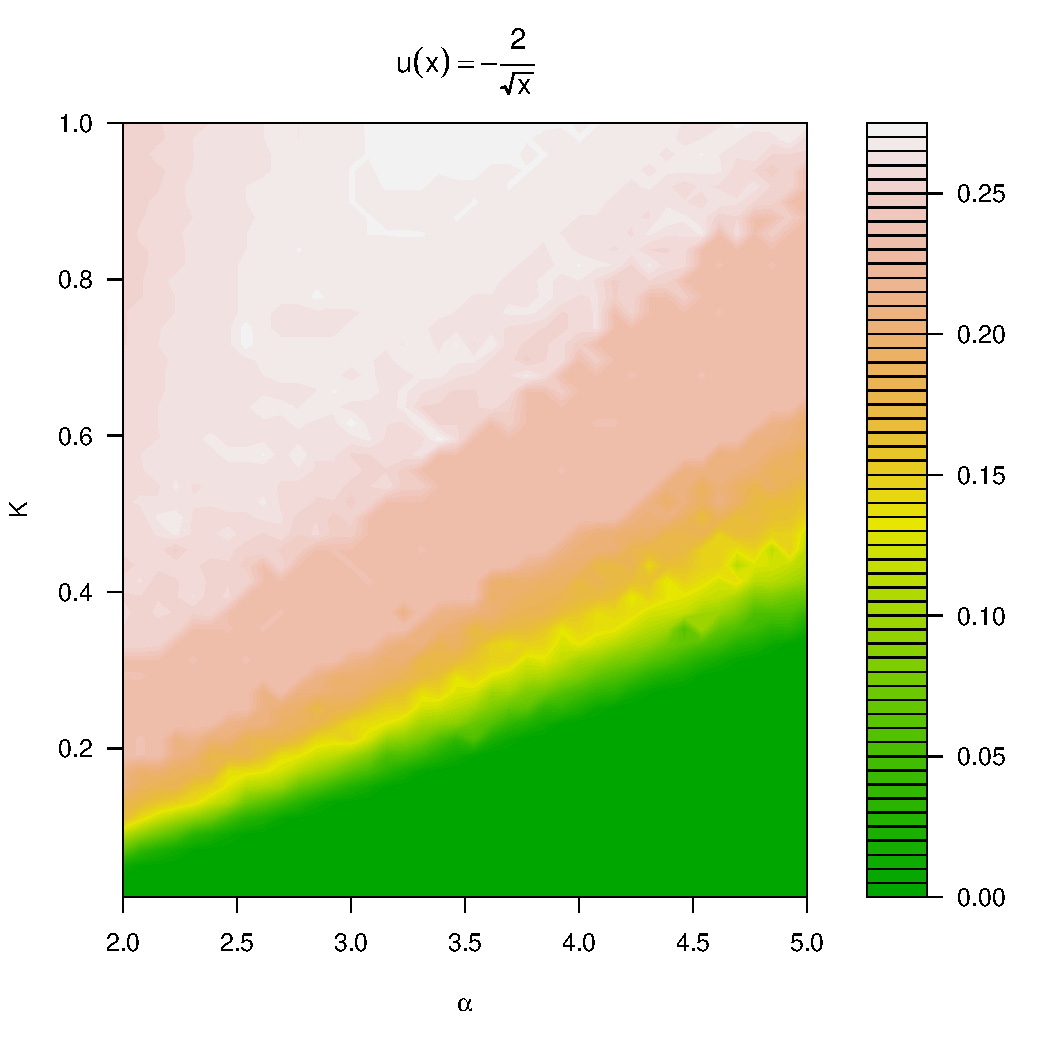
\includegraphics[width=\textwidth]{phi_hat_pareto5e-1.pdf}    
  \end{minipage}\hfill
  \begin{minipage}{0.5\linewidth}
    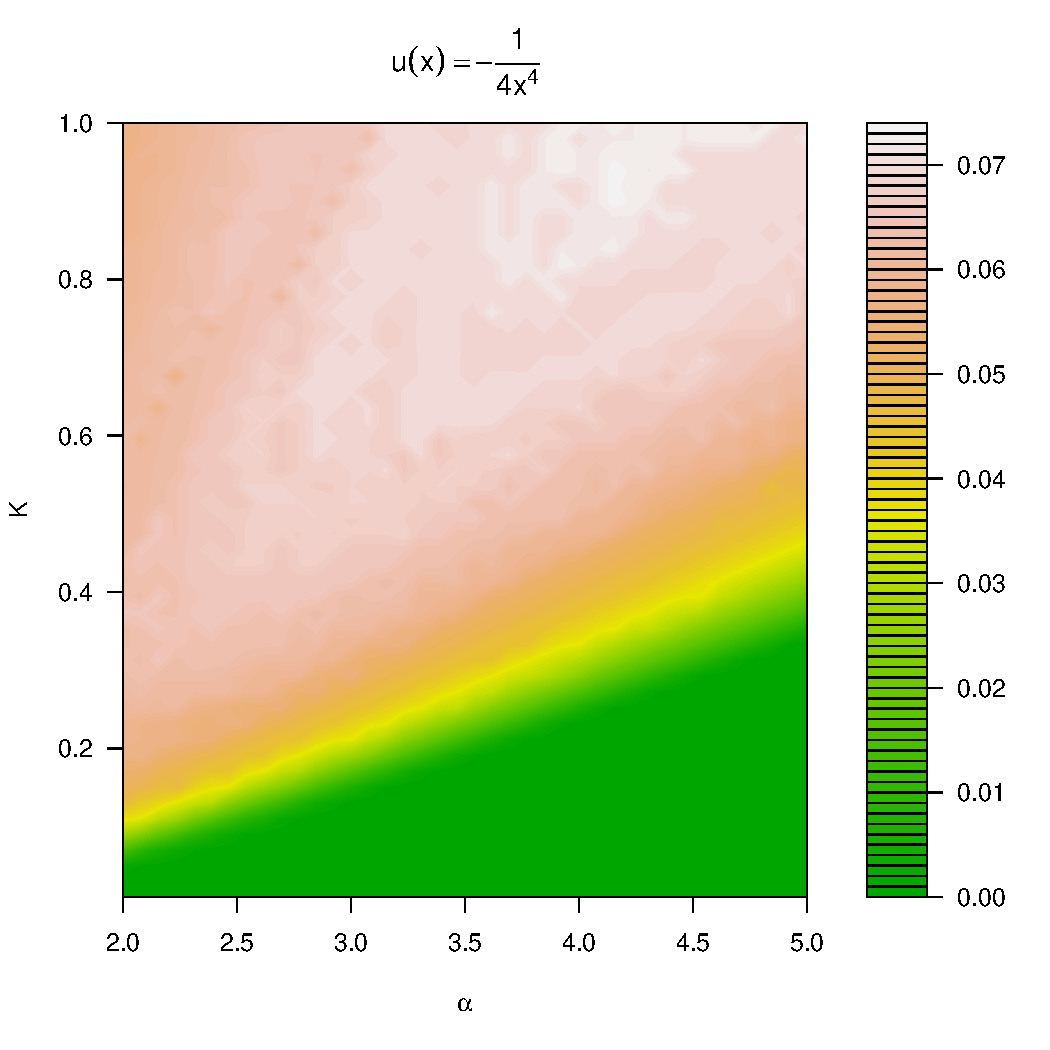
\includegraphics[width=\textwidth]{phi_hat_pareto4.pdf}
  \end{minipage}
  \caption{The graphs show $\hat\phi$, the optimal equity allocation
    as a \fct\ of $\alpha$ and $K$ in the two-sided Pareto model
    \eqref{eq:pareto} with $K=K'$, $\alpha=\beta$. We choose
    the utility $u$ from \eqref{eq:u}
    function $u(x) = -x^{-\xi}/\xi$ for $\xi = 1/2$ (left) and $\xi = 4$
    (right).
  }
  \label{fig:phi_hat_pareto}
\end{figure}

\begin{minipage}{0.5\linewidth}
  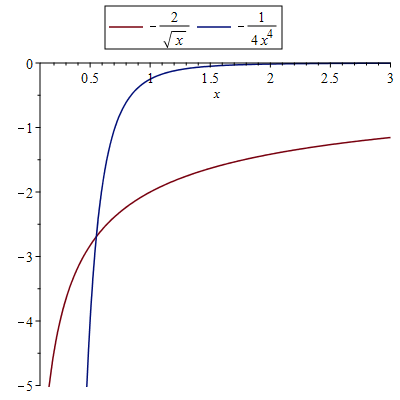
\includegraphics[width=\textwidth]{power_utilities.png}
\end{minipage}\hfill
\begin{minipage}{0.42\textwidth}
  In this graph we show two power-utility functions $u$. We see that
  $u(x)$ grows slower and saturates later for small $\xi$ than for
  large $\xi$. The latter case represents an agent who is more
  tolerant about low consumption and seeks wealth more
  aggressively. In other words, he is less risk-averse than one with a
  larger $\xi$. Such an agent will therefore invest more heavily in
  equity, as shown in Figure~\ref{fig:phi_hat_pareto}.
\end{minipage}

\begin{figure}[htb!]
  \begin{minipage}{0.5\linewidth}
    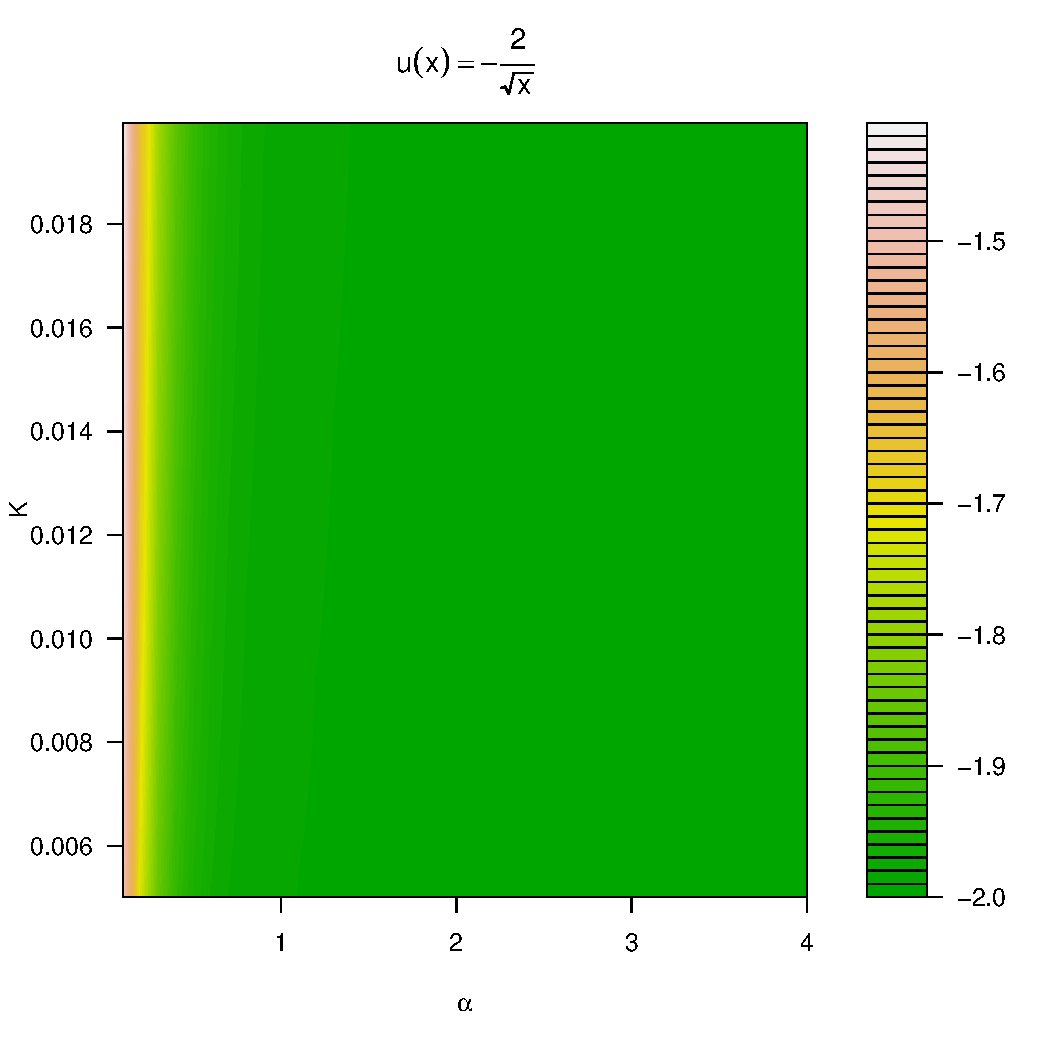
\includegraphics[width=\textwidth]{preference_pareto5e-1.pdf}
  \end{minipage}\hfill
  \begin{minipage}{0.5\linewidth}
    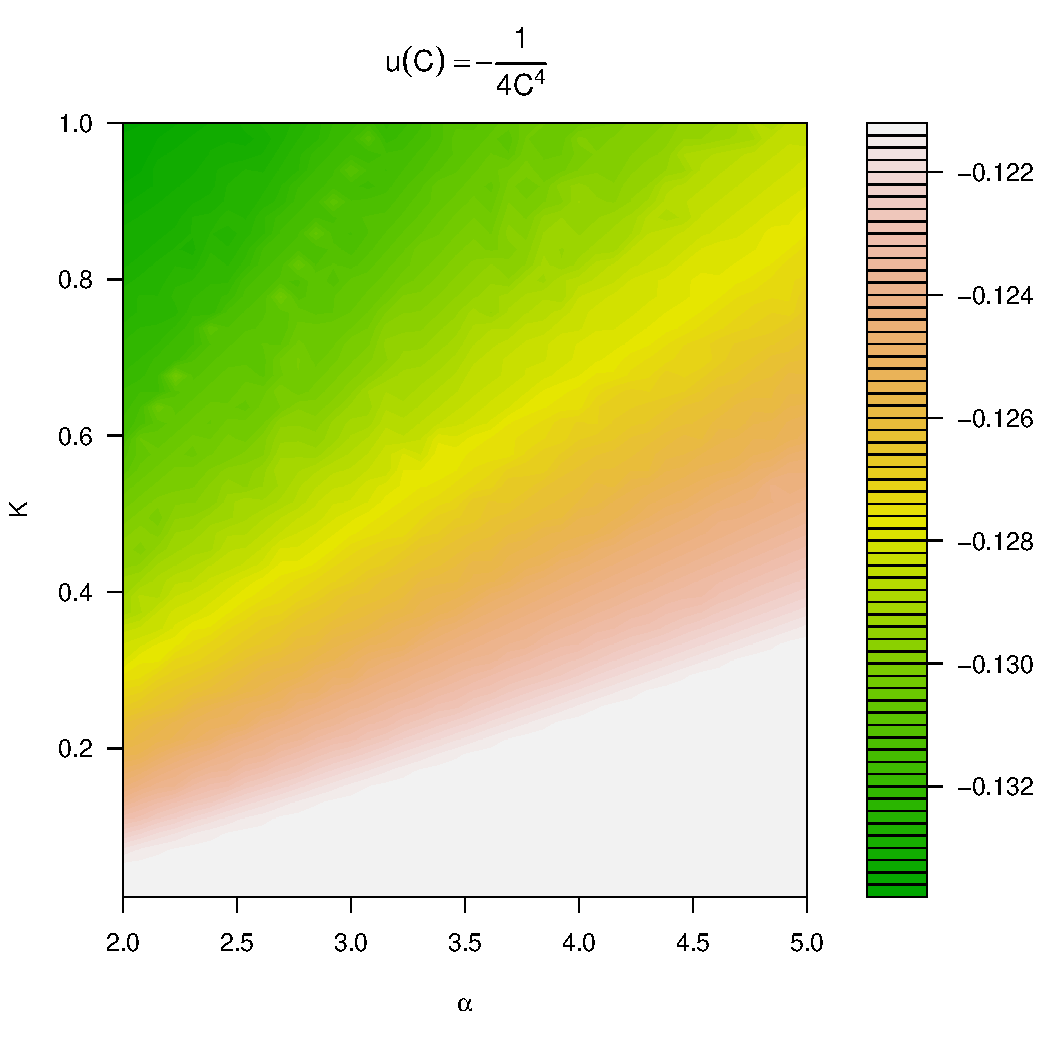
\includegraphics[width=\textwidth]{preference_pareto4.pdf}
  \end{minipage}
  \caption{The quantities $I(\alpha, K)$ for the power-utility \fct\ with $\xi=1/2$ (left) and $\xi=4$ (right).
The graphs clearly show that  $I(\alpha, K)$ increases with $\alpha$ and decreases with $K$.
  }
  \label{fig:preference_pareto}
\end{figure}

\subsection{Student's t-distributed equity return}
It is a common practice to use Student's t-distribution to model the
stationary distribution of equity returns. So it is of interest to
find out what implications this distribution has when it is combined
with the PDA preference. Formally we assume
\[
f(x; \nu) = c(\nu) \left(
  1 + {x^2 \over \nu}
\right)^{-(\nu + 1)/2}
\]
where $\nu > 1$ and
\[
c(\nu) = {
  \Gamma({\nu + 1 \over 2})
  \over
  \Gamma(\nu/2) \sqrt{\nu \pi}
}
\]
We can write $\wt u(F, \phi)$ as
\begin{eqnarray}
  && \wt u(F, \phi) \nonumber \\
  &=&
  \int_{0}^{\infty}
  \left[
    u(C(x, \phi)) + (1 + b)u(C(-x, \phi))
  \right]
  f(x, \nu) dx \nonumber \\
  &&
  + b \int_{0}^{q}
  u(C(x, \phi))
  f(x, \nu) dx - b u(C(q, \phi)) F(q, \nu)
  \label{eq:t1}
\end{eqnarray}
where $C(\cdot)$ is defined in \eqref{eq:xxie1}.

\subsubsection{log-utility function}
We first consider the case where the utility function is simply
$u(\cdot) = \ln(\cdot)$. This corresponds to the limiting case of
\eqref{eq:u} as $\gamma \to 0$.

First notice that when $b = 0$, $\wt u(F, \phi)$ reduces to
$\E u(C(X, \phi))$. Only the first integral of \eqref{eq:t1} remains.
Its integrand becomes $\ln[C(x, \phi) C(-x, \phi)]$.
Now observe $\ln(C(x, \phi)C(-x, \phi))$ is an increasing function of
$x$:
\begin{eqnarray*}
  {\pd C(x, \phi) C(-x, \phi) \over \pd x}
  &=&
  \phi e^r (1 - \phi) (e^x - e^{-x}) > 0
\end{eqnarray*}
Thus when $b = 0$, by 1st case of remark \ref{remark:I} and lemma
\ref{lemma:II},
${\pd \wt u(F, \phi)) \over \pd \nu} < 0$ for all $\phi$. Hence all
investors guided by this utility function would be seeking the
smallest $\nu$, i.e. the heaviest tail in the market. Here note that
Student's t is a symmetric distribution; a heavier tail implies not
only greater down-side risk but also greater up-side potential.

In fact, even when $b > 0$, the same monotonicity property holds. This
is revealed by numerically maximizing $\wt u(F, \phi)$ with
respect to $\phi$ for a sequence of selected values of $\nu$. The
results are shown in figure~\ref{fig:phi_hat_U}.
\begin{figure}[htb!]
  % \begin{subfigure}[b]{0.5\linewidth}
  %   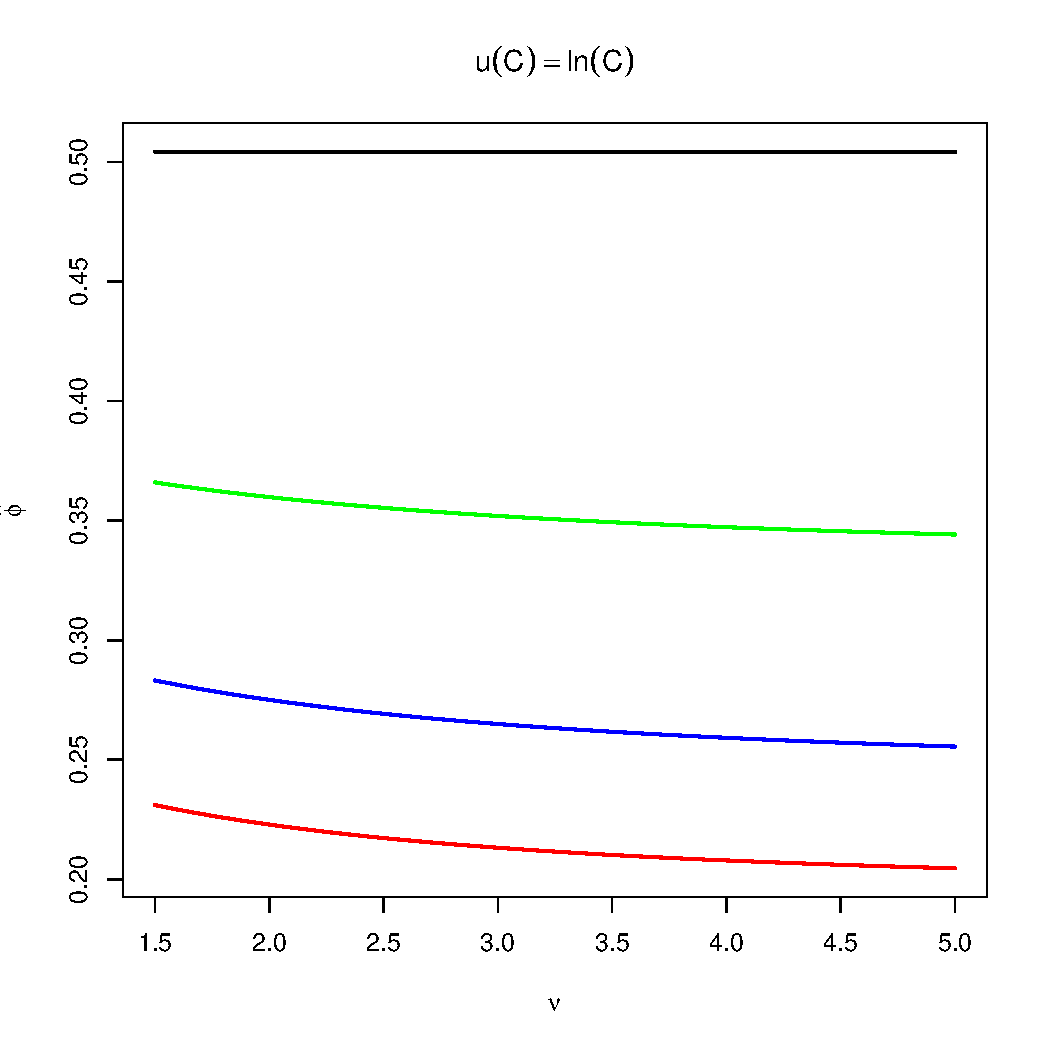
\includegraphics[width=\textwidth]{phi_hat_b_t_log.pdf}
  %   \caption{$\hat\phi(\nu)$ of log-utility function}
  %   \label{fig:phi_hat_t_log}
  % \end{subfigure}
  % \begin{subfigure}[b]{0.5\linewidth}
  %   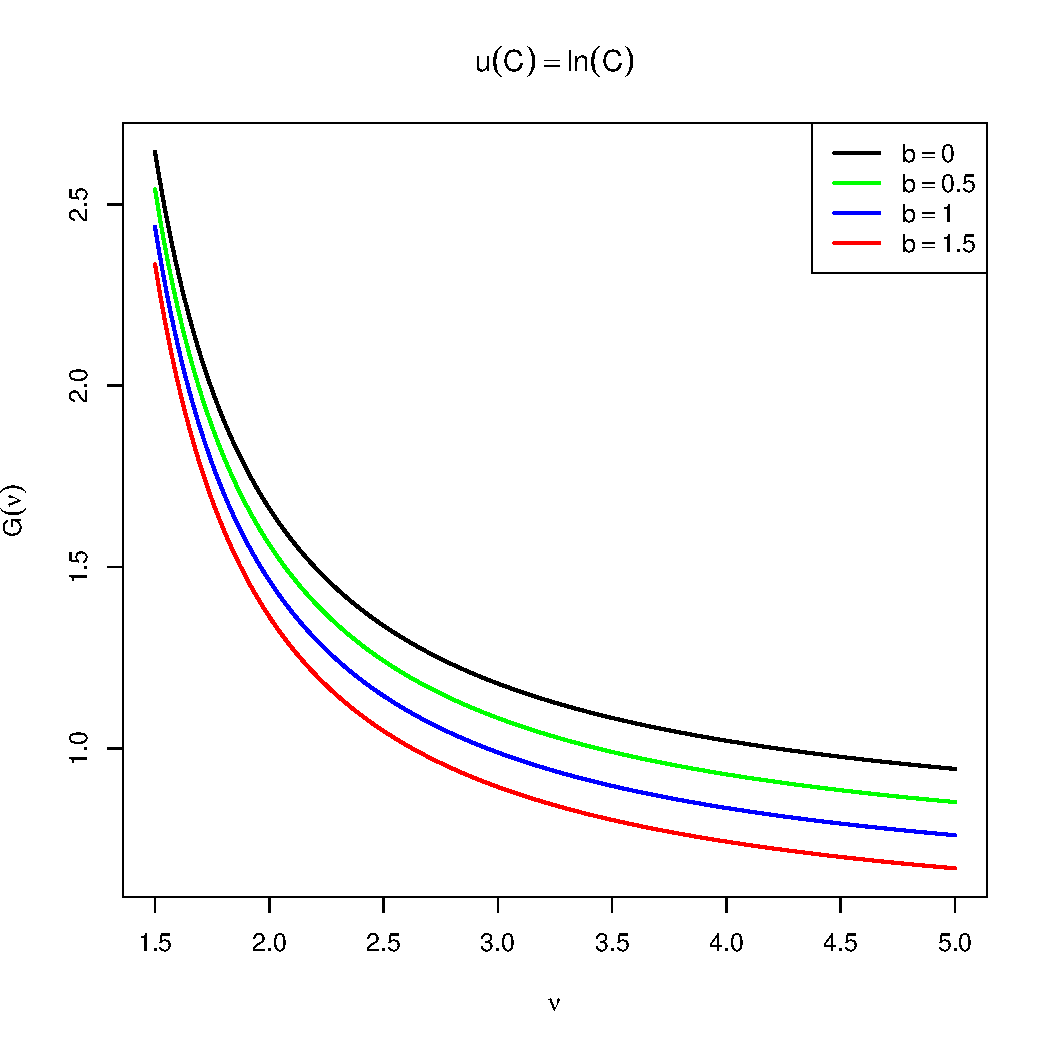
\includegraphics[width=\textwidth]{U_b_t_log.pdf}
  %   \caption{$G(\nu)$ of log-utility function}
  %   \label{fig:U_b_t_log}
  % \end{subfigure}
  % \begin{subfigure}[b]{0.5\linewidth}
  %   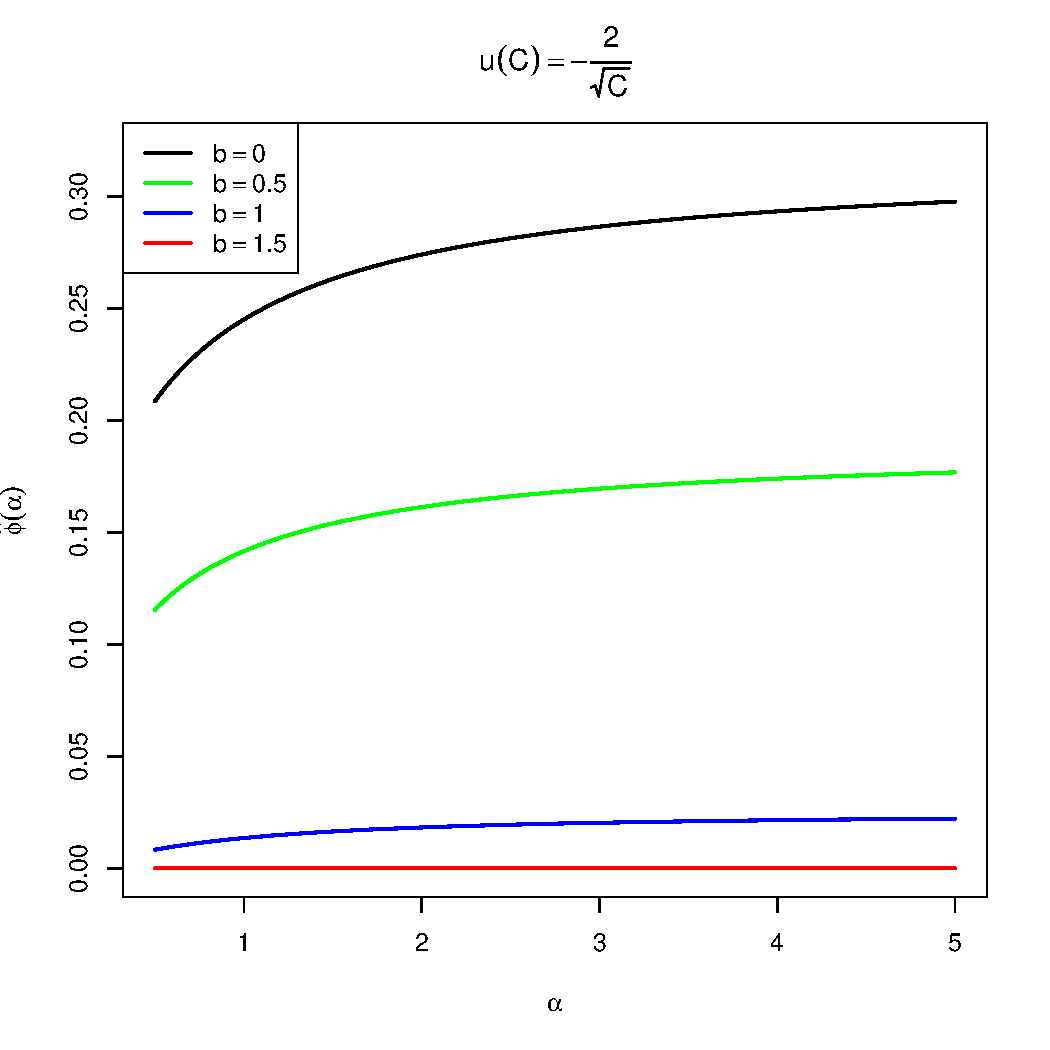
\includegraphics[width=\textwidth]{phi_hat_b_t_power.pdf}
  %   \caption{$\hat\phi(\nu)$ of power-utility function}
  %   \label{fig:phi_hat_t_power}
  % \end{subfigure}
  % \begin{subfigure}[b]{0.5\linewidth}
  %   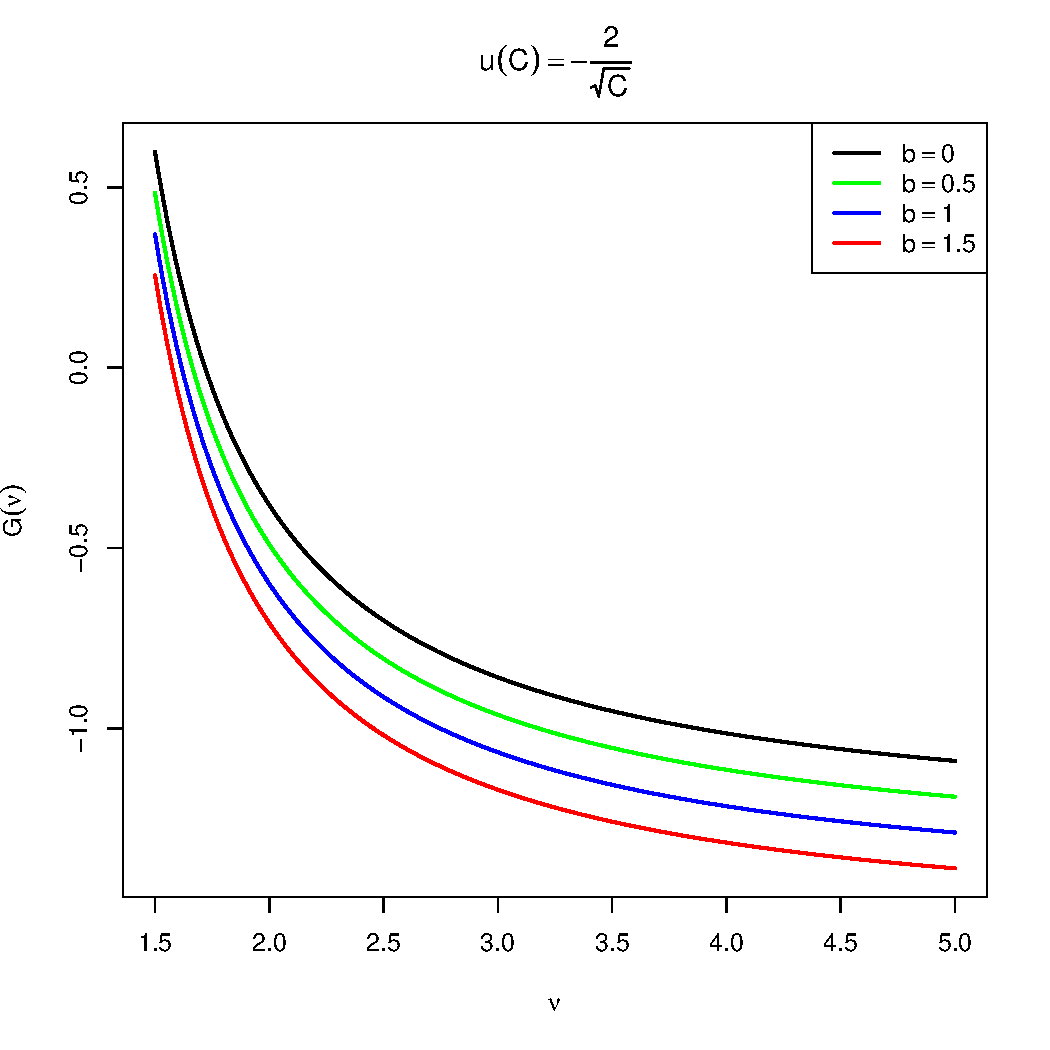
\includegraphics[width=\textwidth]{U_b_t_power.pdf}
  %   \caption{$G(\nu)$ of power-utility function}
  %   \label{fig:U_b_t_power}
  % \end{subfigure}
  \begin{minipage}{0.5\linewidth}
    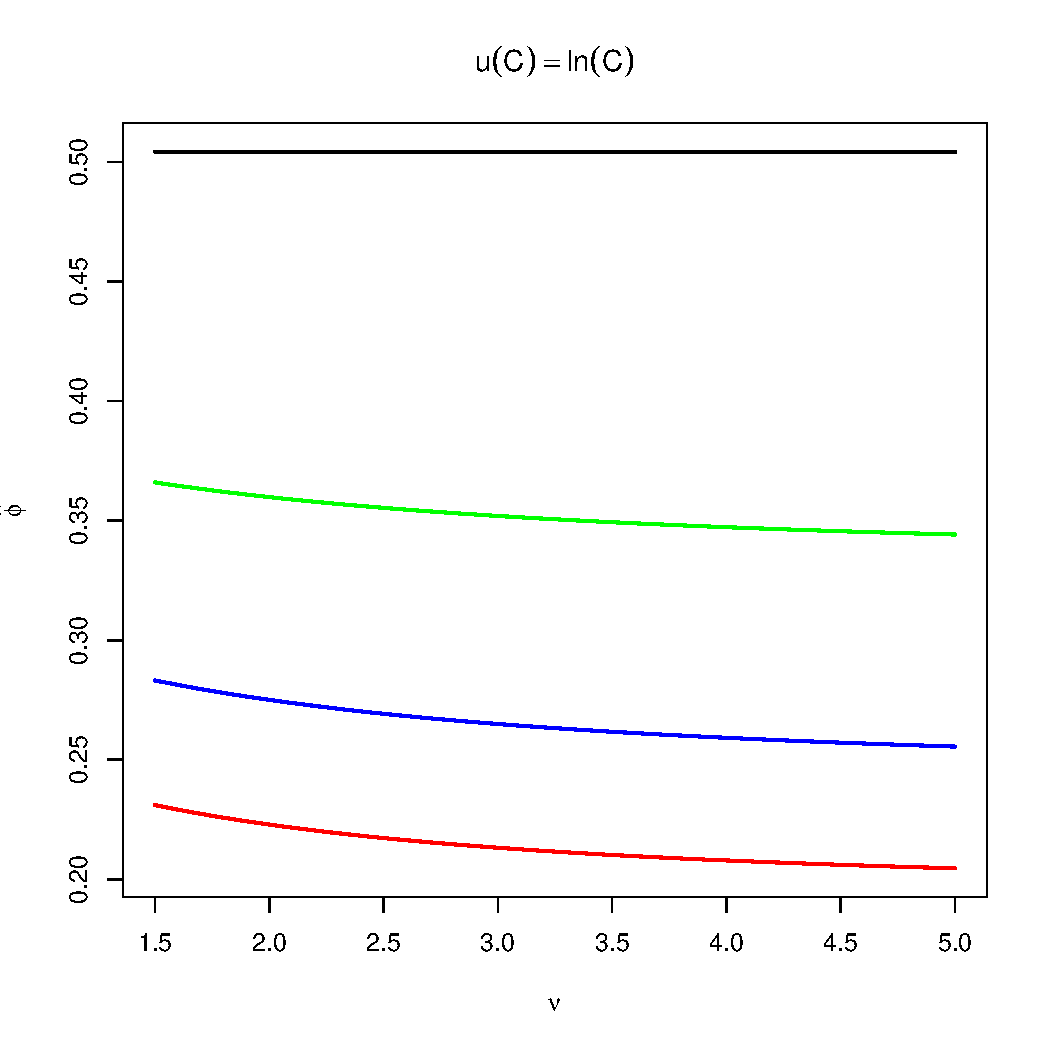
\includegraphics[width=\textwidth]{phi_hat_b_t_log.pdf}
  \end{minipage}\hfill
  \begin{minipage}{0.5\linewidth}
    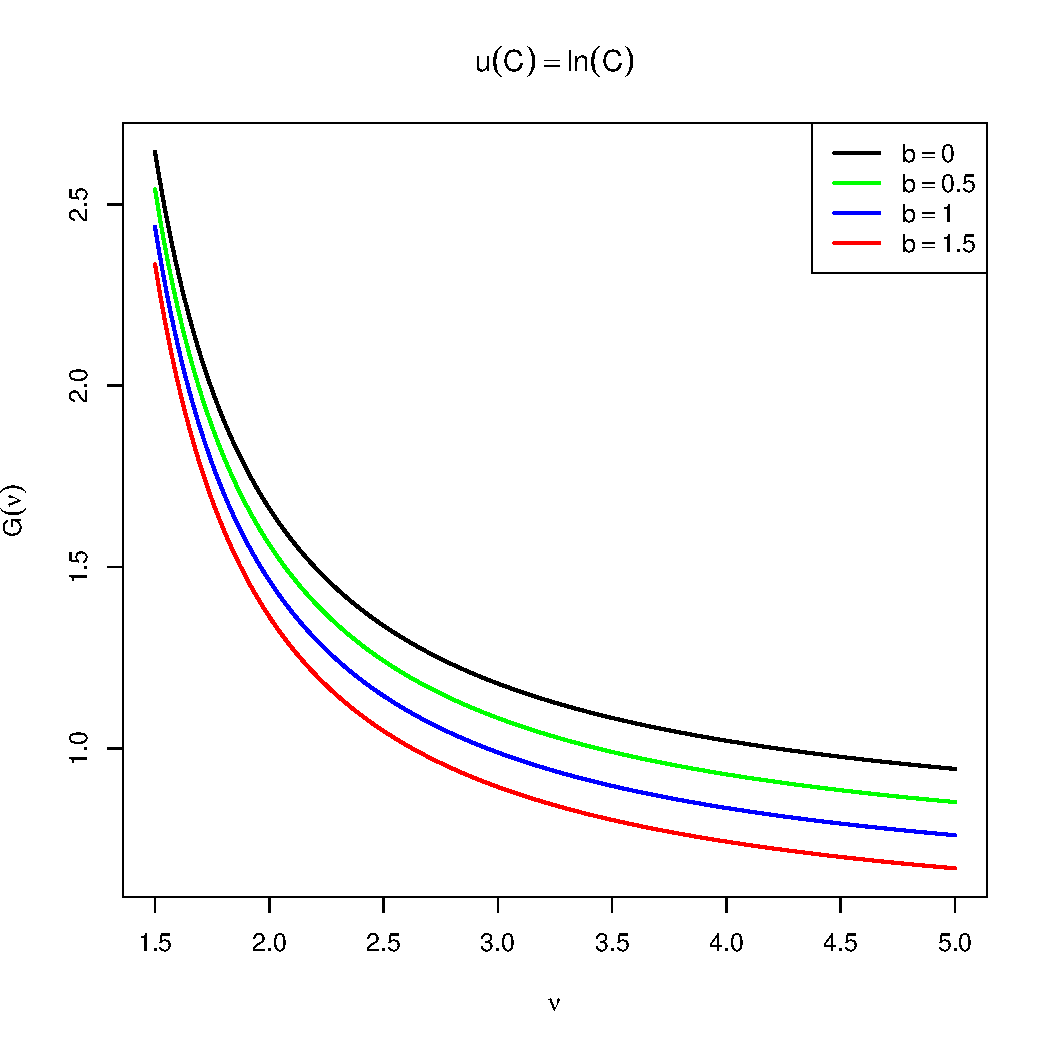
\includegraphics[width=\textwidth]{U_b_t_log.pdf}
  \end{minipage}
  \begin{minipage}{0.5\linewidth}
    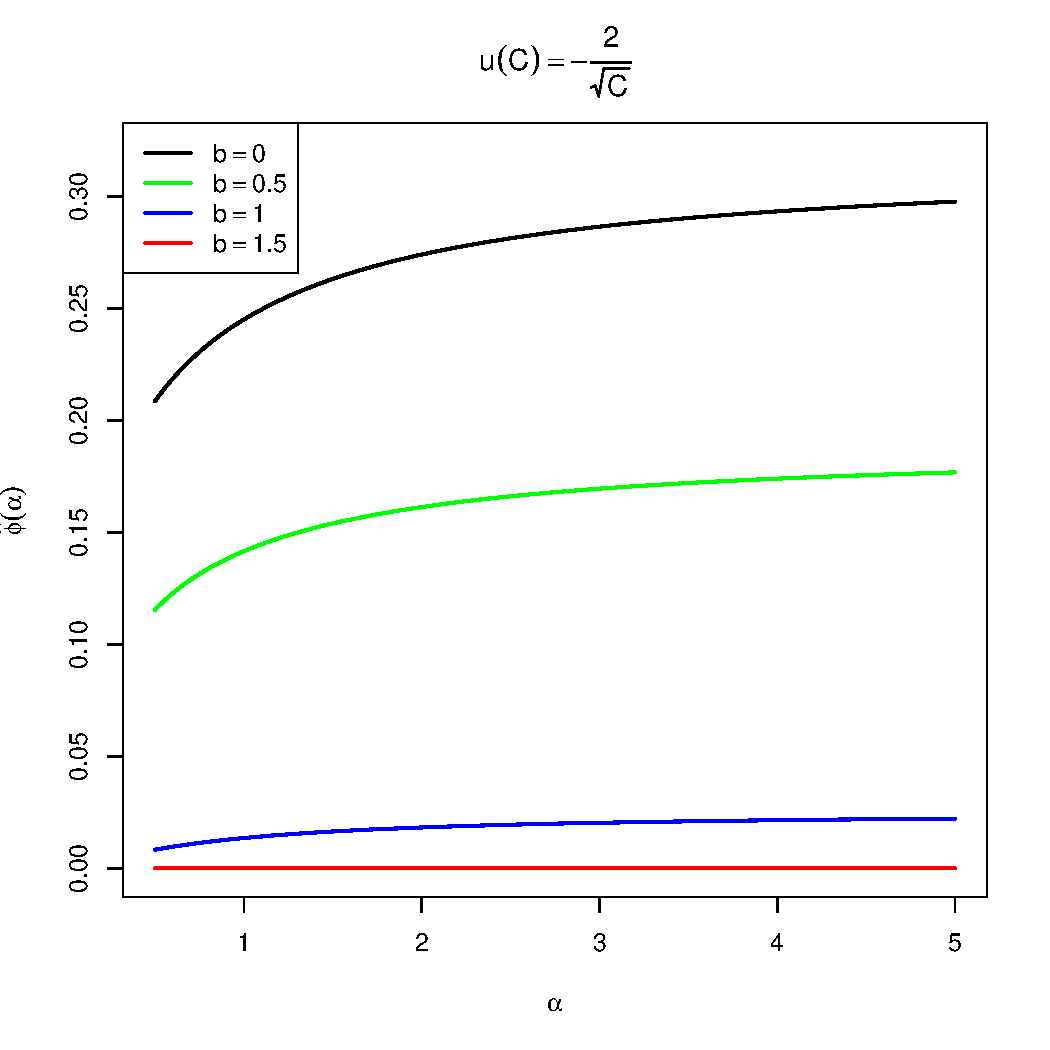
\includegraphics[width=\textwidth]{phi_hat_b_t_power.pdf}
  \end{minipage}\hfill
  \begin{minipage}{0.5\linewidth}
    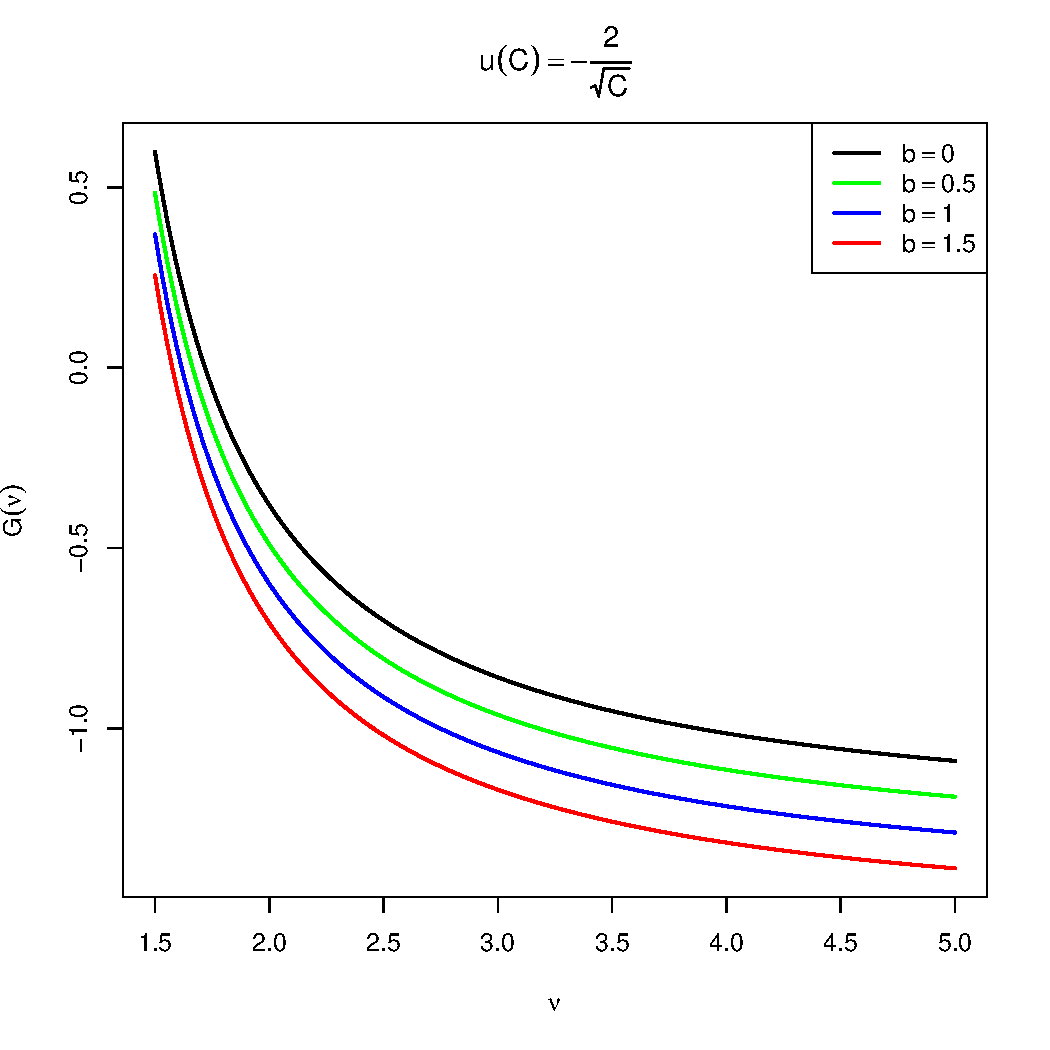
\includegraphics[width=\textwidth]{U_b_t_power.pdf}
  \end{minipage}
  \caption{$\hat\phi$ and $G(\nu)$
    \label{fig:phi_hat_U}
  }
\end{figure}

%% However, this is not necessarily the case when $b > 0$. For example,
%% consider the case when $q = 0$ and $\hat\phi = 1$. This may be
%% viewed an approximation to the situation where the interest rate $r$ is
%% vanishingly low while the investor is more conservative than
%% greedy. In this case we have
%% \begin{eqnarray*}
%%   \wt u(F, \phi) = \int_{0}^{\infty} e^{-b x} f(x, \nu) dx
%% \end{eqnarray*}
%% Thus by the 1st case of lemma \ref{lemma:I} and lemma \ref{lemma:II},
%% $\opd{\nu}\wt u(F, \phi) > 0$. In this extreme case, the investor
%% would rather seek the largest $\nu$ or in other words, the lightest
%% tail in the market.

\subsubsection{power-utility function}
In this section we consider the case when the utility function
$u(\cdot)$ takes the form
\[
u(x) = -{1 \over \xi} x^{-\xi}
\]
One can see from figure \ref{fig:phi_hat_U_power} that both $\hat
\phi$ and $G(\nu)$ are monotonically decreasing with $\nu$ as in the
case of a log-utility function.
\begin{figure}[htb!]
  \begin{minipage}{0.5\linewidth}
    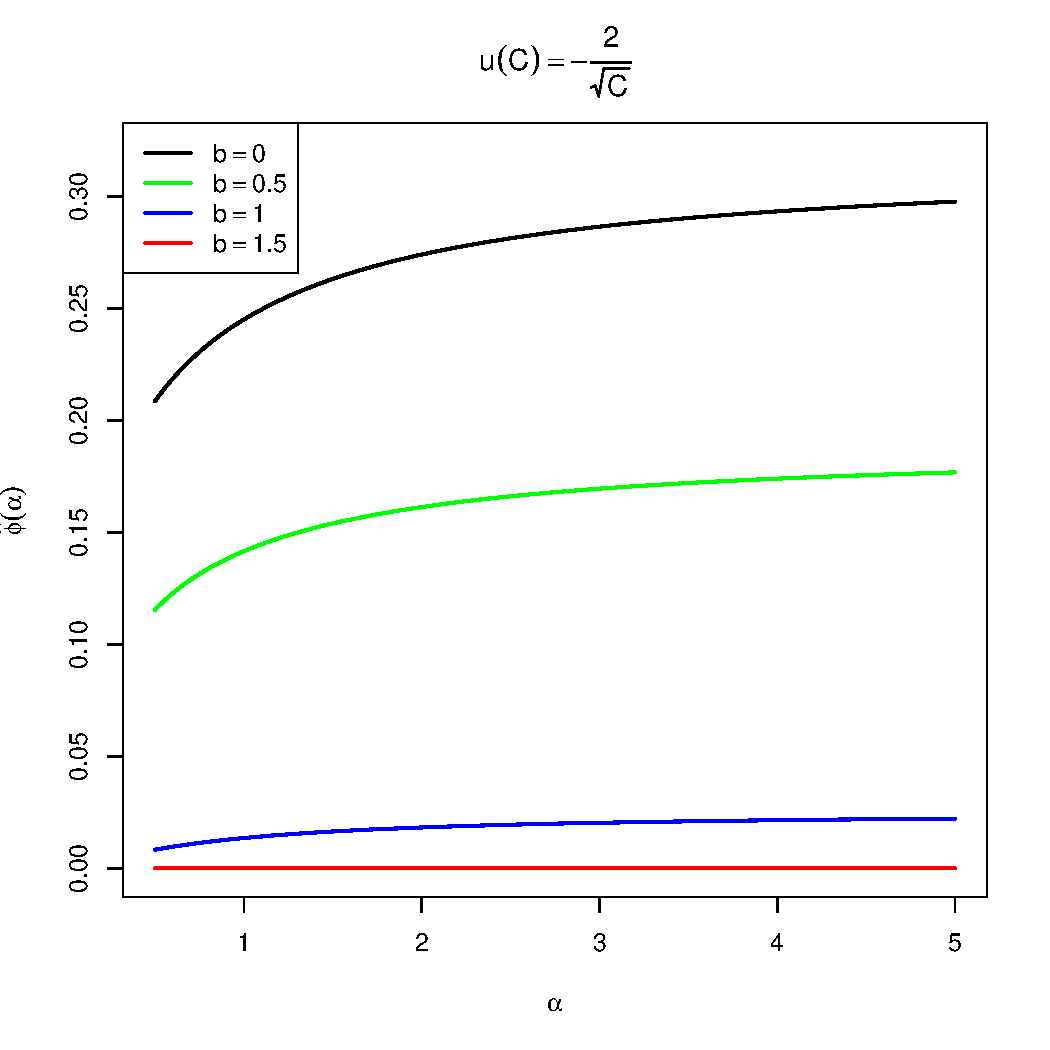
\includegraphics[width=\textwidth]{phi_hat_b_t_power.pdf}
  \end{minipage}\hfill
  \begin{minipage}{0.5\linewidth}
    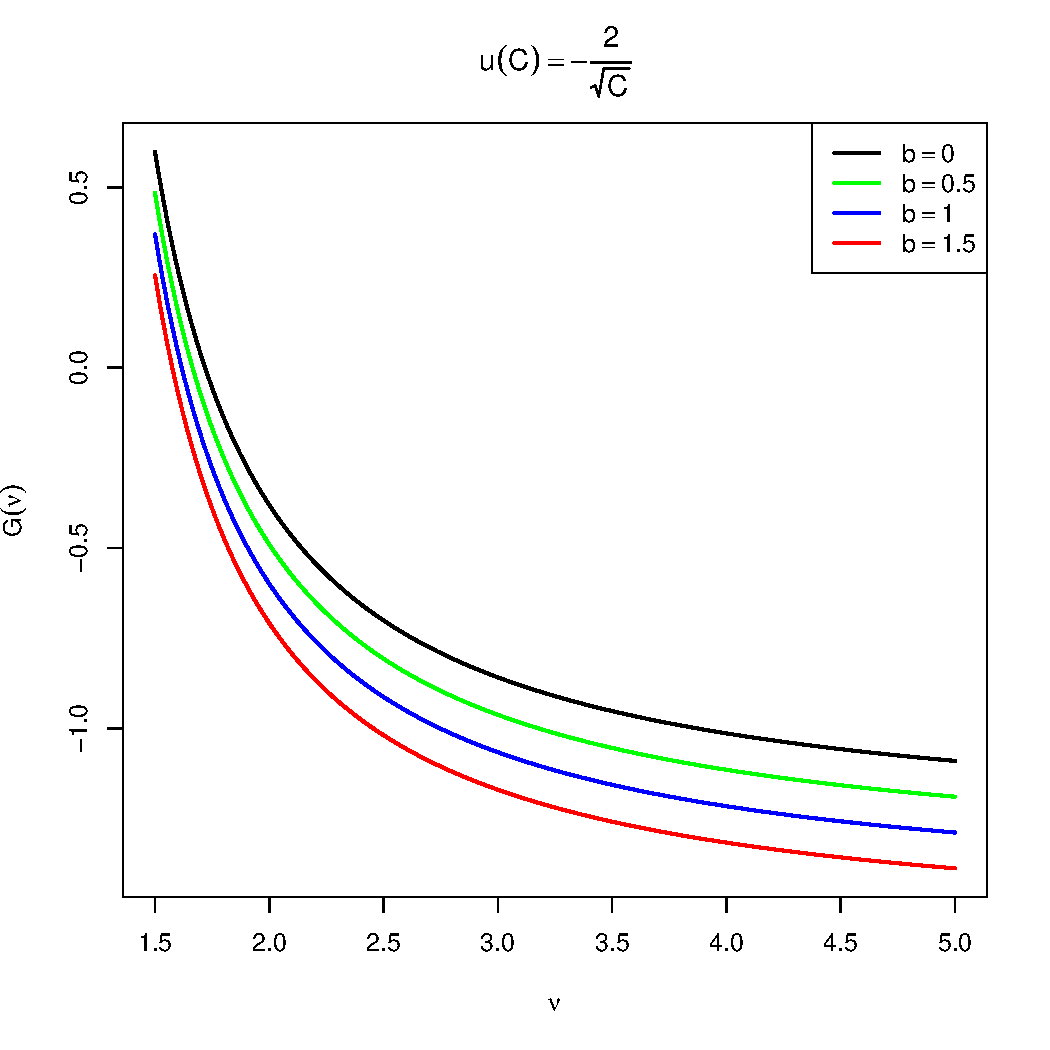
\includegraphics[width=\textwidth]{U_b_t_power.pdf}
  \end{minipage}
  \caption{$\hat\phi$ and $G(\nu)$ when the utility
    function is $u(C) = -{2 \over \sqrt{C}}$
  }
  \label{fig:phi_hat_U_power}
\end{figure}

\section{Conclusion}
\label{sec:4}
TODO: Summarize and conclude that all correlated series share the same
tail index; their tail functions differ from each other via their
scale parameters.

\appendix
\section{A monontonicity lemma}
\begin{lemma} \label{lemma:I}
  Assume distribution function $F(x; \theta)$ parameterized by
  $\theta$ is defined on $x \in (a, b)$, $a, b \in \mathbb R \cup
  \{-\infty, \infty\}$, and in addition $F(x; \theta)$ has density
  function $f(x; \theta)$. Assume function $h(\cdot)$ is defined on
  $(a, b)$, $X \sim F$, $\text{supp}(X) = (a,b)$,
  $\E h(X) < \infty$ and
  \begin{eqnarray*}
    \left| \frac{\pd f(x, \theta)}{\pd \theta} \right| < \infty
    \quad \forall x \in (a, b)
  \end{eqnarray*}
  \begin{enumerate}
  \item If $h(\cdot)$ is decreasing and $\exists x_0 \in (a, b)$ such that
    $\frac{\pd f}{\pd \theta}(x_0; \theta) > 0$ on $(a, x_0)$ while
    $\frac{\pd f}{\pd \theta}(x_0; \theta) < 0$ on $(x_0, b)$, then
    \[
    \frac{\pd \E h(X)}{\pd \theta} > 0
    \]
  \item If $h(\cdot)$ is increasing and $\exists x_0 \in (a, b)$ such that 
    $\frac{\pd f}{\pd \theta}(x_0; \theta) < 0$ on $(a, x_0)$  while
    $\frac{\pd f}{\pd \theta}(x_0; \theta) > 0$ on $(x_0, b)$, then
    \[
    \frac{\pd \E h(X)}{\pd \theta} > 0
    \]
  \end{enumerate}
\end{lemma}
\begin{remark}
  \label{remark:I}
  Two other cases follow trivially from lemma \ref{lemma:I}:
  \begin{enumerate}
  \item If $h(\cdot)$ is increasing and $\frac{\pd f}{\pd \theta}$
    satisfies the
    same conditions of the 1st case of lemma \ref{lemma:I},
    $\frac{\pd \E h(X)}{\pd \theta} < 0$. This immediately follows
    from applying 1st case of lemma \ref{lemma:I} to $-h(\cdot)$.
  \item By the same argument, if $h(\cdot)$ is decreasing and
    ${\pd f \over \pd \theta}$ satisfies the same conditions of the
    2nd case of lemma \ref{lemma:I}, ${\pd \E h(X) \over \pd \theta} < 0$.
  \end{enumerate}
\end{remark}

\begin{proof}
  Clearly
  \begin{eqnarray*}
    && {\pd \E h(X) \over \pd \theta} \\
    &=& \int_a^b h(x) {\pd f \over \pd \theta}(x, \theta) dx \\
    &=& \underbrace{\int_a^{x_0} h(x) {\pd f \over \pd \theta}(x,
      \theta) dx}_{I_1}
    + \underbrace{\int_{x_0}^b h(x) {\pd f \over \pd \theta}(x,
      \theta) dx}_{I_2}
  \end{eqnarray*}
  \begin{enumerate}
  \item When $h(x)$ is decreasing on $(a, b)$ and ${\pd f \over \pd
    \theta}(x, \theta) > 0$ on $(a, x_0)$
    \[
    I_1 > h(x_0) \int_a^{x_0} {\pd f \over \pd \theta}(x, \theta) dx
    \]
    Similarly, because ${\pd f \over \pd \theta}(x, \theta) < 0$ for
    $x \in (x_0, b)$ and $h(x)$ is decreasing, we have
    \begin{eqnarray*}
      I_2 &=& \int_{x_0}^b -h(x_0)
      \left|{\pd f \over \pd \theta}(x, \theta) \right| dx \\
      &>& -h(x_0)
      \int_{x_0}^b \left| 
        {\pd f \over \pd \theta}(x, \theta)
      \right| dx
    \end{eqnarray*}
    Finally we have
    \begin{eqnarray*}
      {\pd \E h(X) \over \pd \theta}
      > h(x_0) \int_a^b {\pd f \over \pd \theta}(x, \theta) dx
      = h(x_0) {\partial \over \partial \theta} \int_a^b f(x, \theta) dx
      = 0
    \end{eqnarray*}
  \item If $h(\cdot)$ is increasing and $\exists x_0 \in (a, b)$ such that 
    ${\pd f \over \pd \theta}(x_0; \theta) < 0$ on $(a, x_0)$  while
    ${\pd f \over \pd \theta}(x_0; \theta) > 0$ on $(x_0, b)$
    \begin{eqnarray*}
      I_1 &=&
      \int_a^{x_0} -h(x)
      \left| {\pd f \over \pd \theta}(x, \theta) \right| dx \\
      &>&
      -h(x_0) \int_a^{x_0}
      \left| {\pd f \over \pd \theta}(x, \theta) \right| dx
    \end{eqnarray*}
    and obviously
    \[
    I_2 > h(x_0) \int_{x_0}^b
    {\pd f \over \pd \theta}(x, \theta) dx
    \]
    So
    \[
    {\pd \E h(X) \over \pd \theta}
    = I_1 + I_2
    > h(x_0) {\partial \over \partial \theta} \int_a^b f(x, \theta) dx = 0
    \]
  \end{enumerate}
\end{proof}

\section{A lemma on Student's t-distribution}
\begin{lemma}
  \label{lemma:II}
  Let $f$ denotes the density function of the Student's
  t-distribution, i.e.
  \[
  f(x; \nu) = c(\nu) \left(
    1 + {x^2 \over \nu}
  \right)^{-(\nu + 1)/2}
  \]
  where $\nu > 1$ and
  \[
  c(\nu) = {
    \Gamma({\nu + 1 \over 2})
    \over
    \Gamma(\nu/2) \sqrt{\nu \pi}
  }
  \]
  Then there exists $x_0 > 0$ such that ${\pd f \over
    \pd \nu}(x_0, \nu) = 0$ and $\forall x \in (0, x_0), {\pd f \over
    \pd \nu}(x, \nu) > 0$ and $\forall x \in (x_0, \infty), {\pd f
    \over \pd \nu}(x, \nu) < 0$.
\end{lemma}
\begin{proof}
  Straightforward computation gives
  \begin{eqnarray}
    {\pd f(x, \nu) \over \pd \nu} &=& {
      c(\nu) x^2 (\nu + 1) + (2 \nu x^2 + 2 \nu^2) c'(\nu)
      -
      \nu c(\nu) (x^2 + \nu) \ln(1 + x^2/\nu)
      \over
      2 \nu (x^2 + \nu) (1 + x^2 / \nu)^{\nu/2 + 1/2}
    } \nonumber \\
    &:=& {
      P(x^2, \nu)
      \over
      2 \nu (x^2 + \nu) (1 + x^2 / \nu)^{\nu/2 + 1/2}
    }
    \label{eq:xxie4.1}
  \end{eqnarray}

  While the denominator of the right side of ${\pd f(x, \nu) \over \pd \nu}$ is
  always positive, its nummerator $P(x^2, \nu)$ has a single root:
  \begin{equation}
    \label{eq:xxie5}
    x_0^2 = \nu\exp\left\{
      W\left[
        -\left(1 + {1 \over \nu}\right)
        e^{-1 - 2 c'(\nu)/c(\nu) - 1/\nu}
      \right]
      + 1 + {1 \over \nu} + {2 c'(\nu) \over c(\nu)}
    \right\} - \nu
  \end{equation}
  where $W(\cdot)$ is the principle branch of the Lambert $W$
  function. and $c'(\cdot)$ is the derivative of $c(\cdot)$. To check
  the right side of \eqref{eq:xxie5} for positivity, we first note
  $c'(\nu) > 0$:
  \[
  c'(\nu) = {
    \pi \Gamma(\nu/2 + 1/2) \left\{
      \nu \left[ \Psi(\nu/2 + 1/2) - \Psi(\nu/2)\right] - 1
    \right\}
    \over
    2 \Gamma(\nu/2) (\pi \nu)^{3/2}
  }
  \]
  where $\Psi(\cdot)$ is the digamma function:
  \[
  \Psi(x) = {d \ln[\Gamma(x)] \over d x}
  \]
  \begin{minipage}{0.48\textwidth}
    $\Psi(x)$ \linebreak
    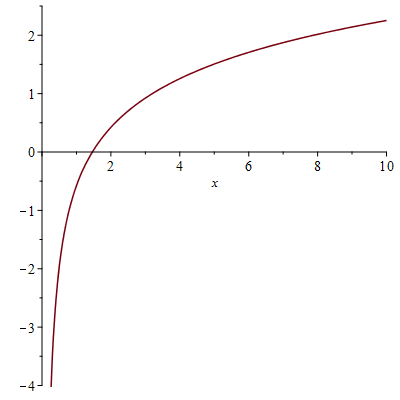
\includegraphics[width=\textwidth]{digamma.png}
  \end{minipage}\hfill
  \begin{minipage}{0.5\textwidth}
    As shown in the figure to the left, $\Psi(x)$ is increasing
    for $x > 0$. This immediately follows from the series
    representation
    \[
    \Psi(x + 1) = -\gamma + \sum_{n=1}^\infty {x \over n(n + x)}
    \quad x \neq -1, -2, -3,\dots
    \]
    which gives
    \[
    {\pd \Psi(x + 1) \over \pd x}
    = \sum_{n=1}^\infty {1 \over (n + x)^2} > 0
    \]
    See Abramowitz and Stegun \cite{abramowitz1972handbook}, p.259,
    formula 6.3.16. Therefore $\Psi(\nu/2 + 1/2) - \Psi(\nu/2) > 0$.
    So we have
    \begin{eqnarray*}
      && \nu \left[
        \Psi(\nu/2 + 1/2) - \Psi(\nu/2)
      \right] - 1 \\
      &\geq& 1 \times \left[
        \Psi(1/2 + 1/2) - \Psi(1/2)
      \right] - 1 \\
      &=& \ln(4) - \ln(e) \\
      &>& 0
    \end{eqnarray*}
    Thus $c'(\nu) > 0$. Furthermore, we recall
    $W(\cdot)$ is increasing on its principle branch. So
  \end{minipage}
  \begin{eqnarray*}
    &&
    W\left[
      -\left( 1 + {1 \over \nu} \right)
      e^{-1 - 2 c'(\nu)/c(\nu) - 1/\nu}
    \right]
    + 1 + {1 \over \nu} + {2 c'(\nu) \over c(\nu)} \\
    &>& 
    W\left[
      -\left( 1 + {1 \over \nu} + {2 c'(\nu) \over c(\nu)} \right)
      e^{-1 - 2 c'(\nu)/c(\nu) - 1/\nu}
    \right]
    + 1 + {1 \over \nu} + {2 c'(\nu) \over c(\nu)} \\
    &=& W(-y e^{-y}) + y
  \end{eqnarray*}
  where
  \[
  y = 1 + {1 \over \nu} + {2 c'(\nu) \over c(\nu)} > 1
  \]
  Now notice
  \[
  \ln(y e^{-y}) = \ln(y) - y
  \]
  is a decreasing function for $y > 1$. Thus $-y e^{-y}$ is an
  increasing function. Hence we have
  \begin{eqnarray*}
    W(-y e^{-y}) + y &>& W(-e^{-1}) + 1 = 0
  \end{eqnarray*}
  Now it is clear
  \[
  \nu\exp\left\{
    W\left[
      -\left(1 + {1 \over \nu}\right)
      e^{-1 - 2 c'(\nu)/c(\nu) - 1/\nu}
    \right]
    + 1 + {1 \over \nu} + {2 c'(\nu) \over c(\nu)}
  \right\} - \nu > 0
  \]
  Now that we have established that ${\pd f \over \pd \nu}(x, \nu) = 0$ has a
  single positive root, it remains to determine the sign of
  ${\pd f \over \pd \nu}(x, \nu)$ on the two sides of the root. For this purpose
  we observe
  \begin{equation}
    \label{eq:xxie5.1}
    P(0, \nu) = 2 \nu^2 c'(\nu) > 0
  \end{equation}
  So we want to investigate ${\pd P \over \pd x}(x, \nu)$:
  \begin{eqnarray}
    {\pd P \over \pd x}(x, \nu) &=&
    2 \nu c'(\nu) + c(\nu) - \nu c(\nu) \ln\left(
      1 + {x \over \nu}
    \right)
    \label{eq:xxie6}
  \end{eqnarray}
  Clearly, $\frac{\pd P}{\pd x}(0, \nu) > 0$. Hence from
  \eqref{eq:xxie5.1} and
  \eqref{eq:xxie6} it is clear
  \begin{equation*}
    \text{sign}\left[
      {\pd f \over \pd\nu}(x, \nu)
    \right]
    = \left\{
    \begin{array}{rl}
      1 & 0 < x < x_0 \\
      -1 & x > x_0
    \end{array}
    \right.
  \end{equation*}
  where $x_0$ is the positive root of \eqref{eq:xxie5}.
\end{proof}

\section{Proof of Remark \ref{thrm:I}}
\label{sec:thrmI_proof}
\begin{proof}
  Let
  \begin{equation}
    \label{eq:xxie2}
    \hat \phi := \underset{0 < \phi \leq 1}{\text{argmax}}\,
    \wt u(F, \phi)
  \end{equation}
  We have
  \[
  G(F) = \wt u(F, \hat\phi)
  \]
  It follows
  \begin{eqnarray}
    {\pd G(F) \over \pd \alpha}
    &=&
    {\pd \wt u(F, \phi) \over \pd \alpha}(\alpha, K, \hat\phi)
    + {\pd \wt u(F, \phi) \over \pd \phi}(\alpha, K, \hat\phi)
    {\pd \hat\phi \over \pd \alpha}(\alpha, K)
    \label{eq:xxie3}
  \end{eqnarray}
  The definition \eqref{eq:xxie2} implies $\forall \alpha > 1$
  \begin{equation}
    \label{eq:xxie4}
    {\pd \wt u(F, \phi) \over \pd \phi}(\alpha, K, \hat \phi) = 0
  \end{equation}
  So the second term of \eqref{eq:xxie3} vanishes. It remains to show
  \begin{eqnarray*}
    {\pd \wt u(F, \phi) \over \pd \alpha}(\alpha, K, \hat \phi)
    &>& 0
  \end{eqnarray*}
  From \eqref{eq:xxie1.0}, it follows
  \begin{eqnarray*}
    {\pd \wt u(F, \phi) \over \pd \alpha}(\alpha, K, \hat\phi)
    = {\partial \over \partial \alpha}\E[u((1 - \hat\phi) e^r + \hat\phi e^X) \1_{\{X < 0\}}]
  \end{eqnarray*}
  The function $u((1 - \hat\phi) e^r + \hat\phi e^X)$ is obviously
  increasing with $X$. It follows
  \begin{eqnarray*}
    && {\pd f(x; \alpha, K) \over \pd \alpha} \\
    &=& {\partial \over \partial \alpha} {\alpha K^\alpha \over (K - x)^{\alpha + 1}} \\
    &=&
    - {K^\alpha \over (K - x)^{\alpha + 1}}
    \left[
      \alpha
      \ln\left(
        1 - {x \over K}
      \right) - 1
    \right]
  \end{eqnarray*}
  It is easily checked that when $x < K(1 - e^{1/\alpha}) < 0$,
  \[
  {\partial \over \partial \alpha} {\alpha K^\alpha \over (K - x)^{\alpha + 1}} < 0
  \]
  and when $K(1 - e^{1/\alpha}) < x < 0$,
  \[
  {\partial \over \partial \alpha} {\alpha K^\alpha \over (K - x)^{\alpha + 1}} > 0
  \]
  This is the second case of lemma \ref{lemma:I}. So we have
  \begin{eqnarray*}
    {\pd \wt u(F, \phi) \over \pd \alpha}(\alpha, K, \hat\phi) &>& 0
  \end{eqnarray*}
  As for ${\pd G(F) \over \pd K}$, by the same argument as for
  ${\pd G(F) \over \pd \alpha}$, it suffices to show
  \[
  {\pd \wt u(F, \phi) \over \pd K}(\alpha, K, \hat\phi) < 0
  \]
  We have
  \[
  {\pd \wt u(F, \phi) \over \pd K}(\alpha, K, \hat\phi)
  = {\partial \over \partial K} \E \left[
    u((1 - \hat\phi) e^r + \hat\phi e^X) \1_{\{X < 0\}}
  \right] 
  \]
  and
  \begin{eqnarray*}
    && {\pd f(x; \alpha, K) \over \pd K} \\
    &=& {\partial \over \partial K} {\alpha K^\alpha \over (K - x)^{\alpha + 1}} \\
    &=&
    -\alpha K^{\alpha - 1} {
      \alpha x + K
      \over
      (K - x)^{\alpha + 2}
    }
  \end{eqnarray*}
  Clearly, when $x < -\alpha/K$
  \[
  {\partial \over \partial K} {\alpha K^\alpha \over (K - x)^{\alpha + 1}} > 0
  \]
  and when $-\alpha/K < x < 0$
  \[
  {\partial \over \partial K} {\alpha K^\alpha \over (K - x)^{\alpha + 1}} < 0
  \]
  So by the 1st case of remark \ref{remark:I} we conclude
  \[
  {\pd \wt u(F, \phi) \over \pd K}(\alpha, K, \hat\phi) < 0  
  \]
\end{proof}

\bibliographystyle{unsrt}
%% \bibliography{../../thesis/econophysics}
\end{document}
